\documentclass[justified]{tufte-book}   	
% use "amsart" instead of "article" for AMSLaTeX format
%\usepackage{geometry}                		% See geometry.pdf to learn the layout options. There are lots.
%\geometry{letterpaper}                   		% ... or a4paper or a5paper or ... 
%\geometry{landscape}                		% Activate for for rotated page geometry
%\usepackage[parfill]{parskip}    		% Activate to begin paragraphs with an empty line rather than an indent
\usepackage{appendix}
\usepackage{graphicx}				% Use pdf, png, jpg, or eps with pdflatex; use eps in DVI mode
\usepackage[plain]{fancyref}								% TeX will automatically convert eps --> pdf in pdflate
\usepackage{amsmath}
\usepackage{mathtools}	
\usepackage{amssymb}
\usepackage{amsthm}
\usepackage[bitstream-charter]{mathdesign}



%\newcommand*{\fancyrefthmlabelprefix}{eq}
\newcommand*{\fancyrefthmlabelprefix}{thm}
\frefformat{plain}{\fancyrefthmlabelprefix}{theorem~#1}
\Frefformat{plain}{\fancyrefthmlabelprefix}{Theorem~#1}
\newcommand*{\fancyrefapplabelprefix}{app}
\frefformat{plain}{\fancyrefapplabelprefix}{appendix~#1}
\Frefformat{plain}{\fancyrefapplabelprefix}{Appendix~#1}
\newcommand{\pd}[2]{\frac{\partial #1}{\partial #2}}
\DeclareMathOperator{\argmin}{argmin}
\DeclareMathOperator{\Tr}{Tr}
\newcommand{\covar}{E}

\title{Optimal Population Coding of Dynamic Stimuli}
\author{Alex Kunze Susemihl}
\date{}							% Activate to display a given date or no date

\begin{document}
\maketitle
\setcounter{tocdepth}{1}
\setcounter{secnumdepth}{1}
\tableofcontents
\chapter{Introduction}

\newthought{Neuroscience as a whole} is concerned with the function of the nervous system. More precisely, it asks a very simple question: {\em What is the brain doing?}\footnote{ Or alternatively: {\em What is the nervous system doing?}} The simplicity with which humans and animals perform in their environment makes it almost unnatural to ask how their brains enable these behaviors. It is often hard to explain to laymen the complexity involved in preparing even the simplest actions, such as saccades or walking, such is the ease with which these are normally performed. Although one can not realistically expect to answer that question in any general fashion, I will try to touch upon a number of points which shed light on some aspects of the nervous system and provide us with a {\em guiding principle} to understand what the brain is doing and why and possibly how.\par
Neuroscience was born as a branch of biology, and although it is now often thought of as  an interdisciplinary science in itself, its objects of study are still to a large extent biological systems. Theodosius Dobzhansky published an influential essay in 1973, entitled {\em Nothing in biology makes sense except in the light of evolution}\cite{Dobzhansky1973}, which defends exactly that point. Though it has been reviewed and revisited constantly since its proposal, the theory of evolution through natural selection remains the central pillar of biological sciences. As such, neuroscience must also view its objects of study through the lenses of evolution. More specifically, we can then ask ourselves {\em What evolutionary advantage would this brain bring to an individual?} instead of {\em Why is the brain this way?} That being said,  there are caveats in the case of neuroscience. For one, the brain is capable of plasticity and adaptation unthinkable for other organs, and so we can not expect to understand the functionality of the brain in the same way in which the shape of bird beaks can be understood as a function of their preferred fruits and seeds. Furthermore, the brain controls all of the motor and perceptual apparatus, having a multitude of uses and purposes, unlike simpler organs.\par
One particular aspect of the brain which has received increasing attention recently is its ability to deal with uncertainty. In a very productive line of research, a number of experiments have demonstrated that human and animal integrate uncertain information in a near-optimal way. The so-called {\em Bayesian Brain}\cite{Knill2004}, would explicitly represent the distribution over world states and perform inference in a manner consistent with Bayesian inference, obtaining optimal integration of sensory cues from different modalities, for example. It is still a matter of debate how these Bayesian computations would be implemented in the brain. One possibility is that the activity of neurons is sampling from a representation of the distribution of world states\cite{Berkes2011}, which is frequently called the {\em sampling hypothesis}. Another is that the activity of the neurons itself represents the likelihood over world states\cite{Ma2006}, and the population as a whole codes for the distribution, hence the term {\em population coding}.\par

\subsection*{Structure}
\newthought{The main goal of this thesis} is to develop a conceptual framework for studying optimal population coding in a dynamic framework. Furthermore, I would like to establish a link between optimal dynamic encoders and the efficient coding hypothesis, first proposed by Horace Barlow\cite{Barlow1961}. I believe that the inclusion of time into the coding framework raises a number of questions, which have not been addressed in the scientific literature properly. In the remainder of this chapter, I will discuss the efficient coding hypothesis and its more recent developments, and I will touch upon its relationship to Shannon's information theory\cite{Shannon1948}. I will finish by discussing the issue of dynamic population coding, highlighting the issues which I believe are of importance in considering the temporal aspect of coding. I will make the case for a study of optimal filtering of partially observed stimuli as a model of stimulus inference based on spike trains. Following, in \fref{chap:filtering}  I will introduce the general theory of filtering of stochastic stimuli. After that, in \fref{chap:MSE} I will discuss results regarding the Mean-Squared-Error (MSE) of optimal filters of point process data, presenting a number of new analytical results. In \fref{chap:control}, I will generalize the filtering framework to control problems, showing results for optimal control theory of point process-observed processes. In \fref{chap:optimal} I will then provide the connection to neuroscience, by considering the optimal encoding strategy for a population of neurons coding for a stochastic stimulus. I will then finalize by discussing the impact of the work presented and suggesting future research directions.\par

\subsection*{Contribution}
\newthought{The main contribution of this thesis} is in providing a conceptual toolbox to study optimal coding problems in a dynamic environment. I propose that the study of the average performance of an optimal Bayesian filter reconstructing the relevant stimulus provides a good measure of the quality of a dynamic code. Using this framework, I derive analytical results for the fast population code for dense populations of Gaussian neurons proposed by Quentin Huys\cite{Huys2007}. These are to my best knowledge the first results of this kind obtained for temporal coding of dynamic stimuli.

\section{Efficient Coding Hypothesis}

\newthought{The information} associated with a random event is defined as the logarithm of its inverse probability. We can further define the entropy of a distribution over a set of events as the average information conveyed by these events. So if we have a random variable $X$ taking values $x \in \mathcal{A}_X$ and a probability distribution $P : \mathcal{A}_X \to [0,1]$, we will have
$$
H(X)= \sum_x P_X(x) \log\left(\frac{1}{P_X(x)}\right).
$$
The entropy measures how much information is gained from a random observation of $X$ on average, and is usually thought of as a measure of the uncertainty or disorder in the distribution $P_X$. Its unit is usually defined as the {\em bit}, derived from binary digit, when the logarithm is taken in base 2. So, a distribution where we have $P_X(x^*) = 1$ for some $x^*$ and $P_X(x) = 0$ for all other $x\neq x^*$ would have an entropy of $0$, since our measurement gives us an average information of $0$. The outcome $x^*$ is completely non-informative, and all other outcomes, while infinitely informative have a zero probability of happening.\par
It can also easily be seen that in the absence of other constraints, if the set of outcomes $\mathcal{A}_X$ is finite, the entropy is maximized by the uniform distribution over outcomes $x$, which would give us the maximal average information per observation of the variable $X$\footnote{We provide a short demonstration in \fref{app:entropy}}. In information theory, the entropy provides the number of bits it takes, on average, to specify an outcome of the random variable $X$.\par
We can now define the conditional entropy of two random variables $X$ and $Y$ as
$$
H(Y|X) = \sum_x P_X(x) \sum_y P_Y(y|x) \log\left(\frac{1}{P_Y(y|x)}\right),
$$
i.e. the conditional entropy is the average entropy of $Y$ given $X$, averaged over $X$. This gives us the remaining uncertainty in $Y$ after $X$ has been observed averaged over all outcomes of $X$, or alternatively, the number of bits required to code for an outcome of $Y$ given an outcome of $X$, on average. Let us also define the mutual information between $Y$ and $X$ as
$$
I(X;Y) = H(Y) - H(Y|X) = H(X) - H(X|Y) = I(Y;X).
$$
In line with our interpretation of the conditional entropy, this would give us the average reduction of uncertainty in $Y$ given the observation of $X$ or vice-versa. Note that, if we fix the distribution of $X$ (or $Y$), the mutual information is always maximized if the conditional entropy $H(X|Y)$ (or $H(Y|X)$, respectively) is minimized. It is easy to see that if $P_X(x|y)$ ($P_Y(y|x)$) is given by a one-to-one mapping between $X$ and $Y$, the conditional entropy is zero, as no uncertainty is left in $X$ after the observation of $Y$ (no uncertainty in $Y$ is left after the observation of $X$).\par
Shannon regarded a noisy communication channel as a set of two random variables, one representing the codeword to be transmitted ($X$) and another representing the message received ($Y$). The noise in the channel would then be given by the conditional distribution of received messages given the transmitted codewords ($P_Y(y|x)$). The capacity of this channel is then given by
$$
C = \max_{P_X} I(X;Y).
$$
This is the maximum amount of information we can transmit through a noisy channel given by the distribution $P_Y(Y|X)$.
The rate of a given code is given by the number of bits needed to represent $X$ divided by the number of bits needed to represent $Y$, so if to send a one-bit message $x$ we must transmit a three-bit codeword $y$, our code would have a rate of $1/3$.
The noisy-channel coding theorem\cite{mackay2003information} then states
\newtheorem{noisychannel}{Theorem}
\begin{noisychannel}
\label{thm:noisychannel}
For every discrete memoryless channel with capacity $C$, for any $\epsilon>0$, any rate $R<C$, and for large enough $N$, there exists a code of length $N$ and rate $\leq R$ and a decoding algorithm such that the maximal probability of block error is $\epsilon$.
\end{noisychannel}
Before Shannon's work, it was generally believed that to achieve a vanishingly small error one would need a code with vanishingly small rate. The theorem shows, however, that one can achieve any rate below the channel capacity asymptotically.\par
Shannon's work had profound impacts throughout science and technology. Horace Barlow proposed to use the redundancy of a code as a measure of its inefficiency. The redundancy of a code is given by
$$
\mathcal{R} = 1 - \frac{I(X;Y)}{C},
$$
and it quantifies how {\em efficiently} a given code encodes codewords $x$ into messages $y$. Note that in the case of a noiseless channel, this reduces to 
$$
\mathcal{R} = 1 - \frac{H(X)}{C}= 1 - \frac{H(Y)}{C}.
$$
The limit given by \fref{thm:noisychannel} then gives us the perfect redundancy-free channel. The {\em efficient coding hypothesis}, first proposed by Barlow\cite{Barlow1961} states that sensory relays in the nervous system recode the	messages to reduce the redundancy in them. This allows us to relate the distribution of the codewords in nature, given by the stimulus statistics, to the firing statistics of the nervous system.\par
In one popular example, Simon Laughlin related the distribution of contrasts in the natural environment of the blowfly to the tuning function of the large monopolar cells (LMC's) in the blowfly's visual system\cite{Laughlin1981}. These cells respond to the contrast level in a specific area of the visual field.
Since we are considering only one neuron, the analysis is somewhat simplified. Let us also assume that the activity of the neuron $o$ can be restricted between no response and a maximal response $o_{max}$. We can then write the activity of the neuron as a function of the contrast $c$ as $o = g(c)$. We will then have that the redundancy of the firing is given by
$$
\mathcal{R} = \frac{1}{C} \left(C - H(O) \right),
$$
which is maximized when all output levels are equally probable.
The transformation from contrasts to firing rates can be written as a simple change of variables and we have, after setting $P(o) = \alpha$\marginnote{This is a reverse application of the inverse transform method.}
$$
P(o) do = P(c) dc, \textrm{ and therefore } o(c) = \frac{1}{\alpha} \int_{-1}^c P(c') dc',
$$
as is shown in \fref{fig:laughlin}. This can be generalized to a number of cases, and Atick\cite{Atick1992} provided a thorough review of the framework.\par

\begin{marginfigure}
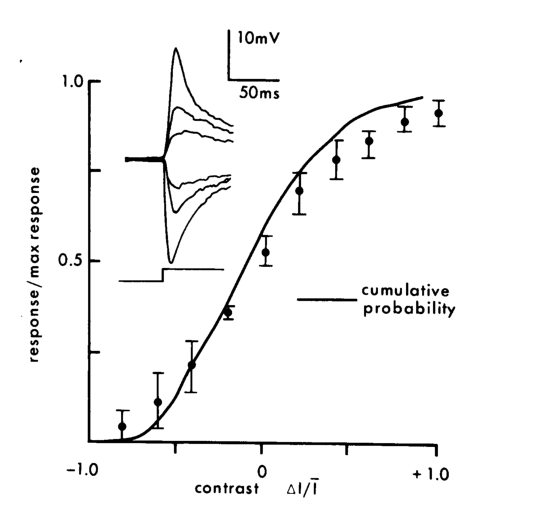
\includegraphics[width=\columnwidth]{figures/laughlin_81.eps}
\label{fig:laughlin}
\caption{The response function of the blowfly LMC closely resembles the cumulative distribution of visual contrasts in its natural environment. Figure taken from Laughlin, S. (1981)}
\end{marginfigure}

This framework can also be generalized to a population of neurons. Writing $O_i$ for the random variable associated with the output activity of each neuron and $O$ for the population activity, we can decompose the redundancy into two terms, yielding
$$
\mathcal{R} = \frac{1}{C} \left(C - \sum_i H(O_i) \right) + \frac{1}{C}\left(\sum_i H(O_i) -H(O)\right).
$$
The first term accounts for redundancy arising from unequal frequency of use of different symbols and the second accounts for redundancy arising from correlations between the activities $O_i$. In the example above we have only had to deal with the left term, since we had only one activity and therefore no correlations between them. A lot of the efficient coding literature, however, has dealt with the second term, and a number of different approaches have looked towards independent components of natural stimuli, assuming that whitening or gain control could account for the maximization of the first term.\par
Michael Lewicki\cite{Lewicki2002}, for example, demonstrated that using independent component analysis\footnote{Indepedent Component Analysis, or ICA for short, tries to decompose a signal into a set of features which are statistically independent between them. This can be done by minimization of a number of different cost functions.} on a set of natural sounds, comprised of human speech, animal vocalizations and natural background sounds, one recovers receptive fields similar to the receptive fields of early auditory neurons. There have been a number of similar studies based on different efficiency measures. A particular popular alternative can be found in the sparse coding literature. Here it is argued that the best possible representation of the natural stimuli is such that only a few neurons are active at a time. Bruno Olshausen and David Field\cite{Olshausen1996}, for example, have shown that, applying the sparse coding approach to a set of natural images results in filters similar to receptive fields in primary visual cortex\footnote{Sparsity is usually measured by the kurtosis of the distribution of activations.}.\par
These results and a number of other similar studies have lent considerable traction to the idea that the nervous system is adapted to encode the stimuli present in the animal's natural environment. This approach, however, is not without its issues. For one, the limit of Shannon's theorem, in which the redundancy of the code is very small, turns the code ever harder to decode. Another important point is that, although minimizing dependence between filters yields good estimates of receptive fields observed in the brain, neurons' activities in the brain are far from independent \footnote{Insert citation about correlations in brain}. Though the redundancy reduction approach has provided numerous insights as mentioned above, other ideas have emerged since.
\par
The finding that humans perform near-optimally\marginnote{Optimality is used in the Bayesian sense, where we mean the subjects integrate uncertain information according to Bayes' rule} when integrating uncertain cues from different senses have led neuroscientists to theorize that the brain explicitly represents distributions over world states\cite{Ernst2002,Ma2006}. In these so-called probabilistic population codes, a spike would contribute to the computation of a posterior probability over world states with a likelihood depending on its conditional probability of firing given the stimulus. This leads to a Bayesian interpretation of the activity of the brain, where the reliability of different sensory cues can be taken in account when integrating them. It can also be argued that representing the uncertainty of events in the world has an important role in decision-making, and will therefore serve as an evolutionary advantage. To use a popular example\footnote{This example is discussed in \citep{Ma2006}.}, let us consider the case of a person deciding wether or not to jump over a stream filled with piranhas. The stream is 1.8 meters wide, and the person jumps an average distance of 2.1 meters. One will be inclined to suggest jumping.\marginnote{Should you jump over a stream filled with piranhas?} Yet both the width of the stream ($w$) as the jumping distance ($j$) are estimated based on uncertain information, and therefore could be imprecise estimates (in the case of the width) or subject to random variation (in the case of the jump distance). Suppose our best guess of the width of the stream is a normal distribution with mean 1.8 meters with a standard deviation of 0.1 meters. Furthermore suppose the standard deviation of the jump distance is 0.4 meters. That would give us a probability of approximately 0.23 of falling down the cliff. So one would definitely be less inclined to jump over the stream, or would at least take preventive actions to minimize the uncertainty in both your estimate of the width of the stream and your jump.\par
From a neural perspective, we could then infer the stimulus distribution (distribution over stream widths) given the response of a neuron population and a model of its response variability. If we assume a given neuron responds according to a certain distribution $P(r|s)$\marginnote{where we term $r$ the response and $s$ the stimulus}, the Bayesian posterior is given simply by
\[
P(s|r) = \frac{P(r|s) P(s)}{P(r)} \propto P(r|s) P(s).
\]
Assuming independent firing for a number of neurons, whose response distributions are given by $P(r_i|s)$ we would have simply
\[
P(s|\{r_1,\ldots,r_n\}) \propto P(s) \prod_i P(r_i|s).
\]
One then still has to determine the nature of the neural variability given by $P(r|s)$. This distribution is often taken to be Poisson. This means that for very short time intervals, of duration $dt$, the probability of neuron $i$ spiking would be given by a rate function $f_i(s)$, as
\[
P_{dt}(r_i|s) \approx f_i(s) dt.
\]
The true Poisson distribution for spike counts assuming the stimulus does not change during a time interval of duration $T$ is given by\marginnote{Poisson distribution}
\[
P_T(r_i|s) = \frac{e^{-f_i(s) T}f_i(s)^{r_i}}{r_i!}
\]
The rate function $f_i(s)$ is often called the tuning function of the neuron. Given a number of neurons in primary visual cortex responding to the edges of the stream, one could then estimate the stream from those responses according to a simple model as
\[
P(width|{r_1,\ldots}) \propto P(width) \prod_i P(r_i|width),
\]
and likewise obtain the mean and standard deviation of our estimate. Note that given a distribution over visual stimuli or a distribution over stream widths, one could seek a set of tuning functions $f_i(s)$ such that the standard deviation of our estimate is minimal. This is clearly a very broad formulation of the problem, but it will be the central question studied in this thesis.

\section{Dynamic Population Coding}

We have had to assume that the stimulus did not change during the response of the neurons to evaluate the Poisson probability of a number of spikes being fired by a neuron. If we relax this assumption, and assume now that the stimulus evolves during time, being now a dynamic stimulus $s(t)$, we will have to reformulate the neural variability model. The probability for infinitesimal time intervals remains the same though. If we denote the number of spikes fired by neuron $i$ since the beginning of the experiment by $N_i(t)$, we can write then
\[
P(N_i(t+dt) - N_i(t) = 1|s(t)) = f_i\left(s(t)\right) dt,
\]
and 
\[
P(N_i(t+dt) - N_i(t) = 0|s(t)) = (1-f_i\left(s(t)\right)) dt.
\]
Denoting the limit with $dt\to 0$ of the difference as $dN_i(t)$, we can write the probability of a spike train given by $N_i = \{N_i(\tau), \tau \in [0,T]\}$ conditioned on the stimulus history $s = \{s(\tau), \tau \in [0,T]\}$ as
\[
P(N_i|s) = \exp\left(-\int_0^T f_i(s(\tau)) d\tau + \int_0^T \log\left[f_i(s(\tau))\right] dN_i(\tau) \right)/N_i(T)!
\]
In that sense we can estimate the probability of the entire stimulus history given a spiking history of a population of neurons as
\[
P(s|\{N_1,\ldots,N_n\}) = P(s) \prod_i P(N_i|s),
\]
furthermore we can marginalize out all but the present value of $s$ to obtain the filtering probability
\[
P(s(T)|\{N_1,\ldots,N_n\}) = \int d\mu(s\setminus T) P(s) \prod_i P(N_i|s)
\]

%The main goal of neuroscience is to answer a simple yet puzzling question: {\em What is the brain doing?} One might argue that we know a lot about what the brain is doing, at least on the phenomenological side, yet the more conceptual levels of what problem the brain is solving, or what it is good at doing, are far from answered. The main analogy we see in use in the field of neuroscience is that of the brain as a computer, hence the frequent use of concepts from Shannon's mathematical theory of communication. Namely, it is frequently hypothesized that the brain is optimally representing interesting aspects of the world it perceives. This thesis seeks to discuss the concept of optimal coding in neural systems. In it, I will discuss mainly findings in filtering of stochastic processes from point process observations and its relation to optimal population coding.\par
%Filtering is of general interest because of its relation to optimal control. More precisely, when considering a linear quadratic control problem under Gaussian noise conditions, the {\em separation principle} holds, and we can design an optimal controller by first predicting the state of the system, and then choosing the optimal control for the noiseless case on that state. The prediction step is solved by the Kalman filter. This framework is frequently used in the study of motor control, and a number of recent experiments and developments have relied on optimal control theory to model the properties of animal subjects under specific noise conditions. Here I will argue that the same approach should also be considered in the sensory areas of the brain.\par
%Investigators have repeatedly hypothesized that the shape of receptive fields and the response properties of sensory neurons can be traced back to optimality with respect to some criterion. The first approach, which drew heavily from Shannon's information theory, was Barlow's efficient coding hypothesis. In its initial form, it stated that the code employed in sensory systems should be adapted to the stimulus distribution in a way to minimized the redundancy, as defined in information theory as the difference between the code capacity and the source entropy divided by the code capacity. Many different efficiency measures have since been proposed. Metabolical considerations favor the use of sparse codes, where at any given time only a few neurons are active.\par
%Another popular approach is to use the Cramer-Rao bound of statistics, and maximize the fisher information of the code, so minimizing a lower bound on the mean-squared-error of the estimator. This has been very popular and is still widely employed in the theoretical neuroscience literature. This bound, however, has been proven to not be tight in useful regimes, and more recently a shift towards using the minimum of the mean-squared-error directly as an efficiency measure has been taking place. We focus here on this measure of efficiency, which we will motivate through optimal control theory in chapter ?? (INSERT REFERENCE).\par
%An alternative approach, which is still in its budding phase, is to consider directly optimal control problems and from the average cost incurred by a given code, choose an optimal code for a given task. This is hindered by the considerable analytical problems involved in treating optimal control problems analytically. I will show, however, that in the popular framework of dense Gaussian tuning functions, an exact expression can be found for the optimal cost-to-go of a linear-quadratic-Gaussian control problem. This bypasses the somewhat abstract notion of an efficiency criterion to consider directly the costs of a given code to the animal using it. It does so at the considerable expense of oversimplifying the problems faced by an animal to an impressive amount. Yet, the approach considers the problem of optimal coding from a more holistic perspective, considering representation and coding as a cog in a machine rather than and end in itself.\par
%
%\section{Structure}
%
%I will start out by reviewing the literature and the different approaches to optimal population coding in chapter ??, giving special attention to the case of mean-squared-error minimization which is considered in this thesis. In the following chapter, I briefly introduce the theory of filtering of point-process observed stochastic processes. Here, the general theory of filtering is presented and the simplifications introduced by the dense Gaussian tuning function limit are discussed. In the following chapter, I discuss results on the mean-squared-error in filtering of Gaussian processes, providing analytical results and comparing it to simulations. The derivations are also compared with a replica-type approach which yields the same results. In the following chapter I consider the problem of optimal control using point-process observations. This is discussed briefly, and a derivation for the optimal cost-to-go is presented. Finally, I consider the implications of the approaches developed to a ecological theory of sensory processing. Namely, I consider the relationship between optimal tuning widths and firing rates with the timescales and correlation lengths in the processes. This is also done numerically for a number of cases that are analytically intractable. I finalize by discussing the presented research, its impact and relation to previous research and future directions of research.
%\cite{susemihl2011}

%We will argue that filtering of stochastic processes is a good proxy for the neural representation of stimuli in the brain.\par

%This presents a number of problems, which we will address in this thesis.

\chapter{Filtering and Prediction with Point Process Observations}

\label{chap:filtering}

\epigraph{Prediction is very difficult, especially about the future.}{Niels Bohr}

In the Introduction I described the general framework in which I seek to study optimal population coding. To do so in a dynamic setting, one must first develop the theory
of temporal estimation of dynamic stimuli from point processes. This is a surrogate for the functioning of a neural population receiving information from the encoder.
There are a number of cases in which the filtering problem can be solved exactly, and I will discuss results from the theory of optimal filtering. In the cases where the
optimal filter is intractable or too expensive to evaluate exactly, I will present methods to approximate the posterior density.\par

In the neuroscientific context, the process $X(t)$ being estimated or filtered would correspond to some environmental feature of interest to a sensory system of some organism, while
the signal would be some neural response coming from a neural population. As was mentioned in \fref{sec:framework}, one example would be to estimate the presence of a moving
grating from the response of retinal ganglion cells. In that sense, the ganglion cells provide a noisy representation of an environmental variable of interest to some downstream
cortical area (V1 for example). In this chapter I will discuss methods to infer the value of the sensory stimulus from the noisy response of a population of neurons.

\section{A Note on Stochastic Processes}

\label{sec:stochastic_proc}

Throughout this thesis, I will repeatedly talk about stochastic processes and the framework of stochastic calculus, so I will provide a short introduction to stochastic processes and
the theory of stochastic calculus. In the study of ordinary differential equations, one works with equations such as
\[
\frac{d x}{dt} = f(x),
\]
which are solved by
\[
x(t) = x(0) + \int_0^t f(x(u),u) du.
\]
This can be modified to include a white-noise term in the evolution of $x(t)$, leading to the Langevin equation
\[
\frac{d X}{dt} = f(X,t) + \sigma(X,t) \xi(t),
\]
where $\sigma(X(u),u)$ is a state- and time-dependent strength and $\xi(t)$ is a {\em rapidly fluctuating random term}, i.e.\mycite{Gardiner2004}
$$\boldsymbol{E}[\xi(t)] = 0\textrm{ and }\boldsymbol{E}[\xi(t)\xi(s)] = \delta(t-s).
$$ 
This approach is 
problematic, however, since the process $X(t)$ thus defined is not differentiable, rendering the Langevin equation mathematically inconsistent. One can, however, extend the solution 
to the deterministic case as
\footnote{Note that because of the new definition, $X(t)$ is now a random variable, hence
the upper-case notation.}
\[
X(t) = X(0) + \int_0^t f(X(u),u) du + \int_0^t \sigma(X(u),u) \xi(u) du.
\]
$\xi(u)du$ can be shown to be equal to $dW(u) = W(u+dt)-W(u)$ in the limit $dt \to 0$, which leads to the usual It\=o stochastic integral
\[
X(t) = X(0) + \int_0^t f\left(X(u),u\right) du + \int_0^t \sigma\left(X(u),u\right) dW(u).
\]
The stochastic integral can be shown to exist as long as the functions $f$ and $\sigma$ are continuous and non-anticipating.\footnote{A function $G(t)$ is said to be non-anticipating 
with  respect to a stochastic process $X$ if it is statistically independent of values of $X(s)$ for $s>t$. Simply put, $G_n(t) = \int_0^t dW(s)$ is non-anticipating with respect to $W(s)$, but
$G_a(t) = \int_0^{2t} dW(s)$ is not.} One usually writes the evolution of $X(s)$ in terms of a stochastic differential equation, instead of a stochastic integral. The process $X(t)$ 
described above would obey the SDE
\[
dX(t) = f\left(X(t),t\right) dt + \sigma\left(X(t),t\right) dW(t).
\]
This is just a shorthand for the stochastic integral, and has no precise mathematical interpretation, as the terms are of different orders. More specifically, the term $dW(t)$ is of the 
order of $\sqrt{dt}$ while the first term is of order $dt$. In an analogy to the study of classical mechanics, the first term is often called the drift of $X(t)$ and the second the diffusion.
\par

Processes $X(s)$ defined in this way are continuous. Often, however, one wants to model a stochastic process which incurs discontinuous jumps as well. I can for that purpose 
introduce a third term in the definition of $X(t)$. Let $j(X(t),t)$ be a function that describes the size of the jump the process experiences at time $t$ and state $X(t)$. 
If these jumps occur at some set of random times $\{t_i\}$, the process $X(t)$ can be written as
\[
X(t) = X(0) + \int_0^t f\left(X(u),u\right) du + \int_0^t \sigma\left(X(u),u\right) dW(u) + \sum_{t_i <t} j\left(X(t_i^-),t_i\right),
\]
where I have defined
$$
X(t^-) \equiv \lim_{s \uparrow t} X(s),
$$
as the limit of $X(t)$ from the left. The jumps in $X(t)$ should be modulated by the point where they originate, not their
destination, so this definition makes intuitive sense.
Let $N(t)$ be then given by
\[
N(t) = \sum_{t_i} \Theta(t-t_i) = \int_0^t \sum_i \delta(u-t_i) du\equiv \int_0^t dN(u), 
\]
where $\Theta(x)$ is the Heaviside step function. With this definition, I can then write
\[
X(t) = X(0) + \int_0^t f\left(X(u),u\right) du + \int_0^t \sigma\left(X(u),u\right) dW(u) + \int_0^t j\left(X(u),u\right) dN(u).
\]
Throughout the text I will also employ an SDE notation for this integral as follows
\begin{equation}
\label{eq:full_stoc}
dX(t) = f\left(X(t),t\right) dt + \sigma\left(X(t),t\right) dW(t) + j\left(X(t^-),t\right) dN(t).
\end{equation}
\par
This encompasses all the stochastic processes I will consider in this text. What happens to a function of a stochastic variable that changes over time, though? Say I want to evaluate
some function of $X(t)$, say $g(X(t),t)$, how does this function vary in time? It\=o's lemma tells one how to find the variation in $g$ from the process $X(t)$. If $X(t)$ evolves according
 to \fref{eq:full_stoc}, we have\footnote{For a more full derivation, see \mycitep{Sennewald2006} or \mycitep{privault2014}.}
\begin{align*}
 dg \equiv& \lim_{dt \to 0} \left[g(X(t+dt),t+dt) - g(X(t),t)\right]\\
 =& \left(\partial_t g + \partial_x g^\top\, f(X(t),t) +\frac{1}{2}\Tr\left[ \sigma\sigma^\top \partial^2_x g\right]\right) dt+ \partial_x f^\top \sigma(X(t),t) dW(t) \\
 &+ \left(g(X(t^-)+j(X(t^-,t),t)-g(X(t^-),t)\right)dN(t),
 \end{align*}
 where I am using the notation
 $$\partial_x g = \left(\frac{\partial g}{\partial x_1},\ldots, \frac{\partial g}{\partial x_N}\right)^\top$$
 and 
 $$
 (\partial^2_x g)_{i,j} = \frac{\partial^2 g}{\partial x_i \partial x_j}.
 $$
This is, again to be understood as a stochastic integral, where we have
\begin{align*}
g(X(t),t) =& g(X(0),0) + \int_0^t \left(\partial_t g + \partial_x g^\top f(X(u),u) +\frac{1}{2}\Tr\left[ \sigma\sigma^\top \partial^2_x g\right]\right) du \\
&+ \int_0^t \partial_x f^\top \sigma(X(u),u) dW(u) +\int_0^t \left(g(X(u^-)+j(X(u^-,u),u)-g(X(u^-),u)\right)dN(u).
\end{align*}
This is in stark contrast of the usual change of variables formula for differentiable variables $y(t)$, where we would have
\[
dg\equiv \lim_{dt \to 0} \left[g(y(t+dt),t+dt) - g(y(t),t)\right]= \left(\partial_t g + \partial_y g^\top \, \partial_t y \right)dt.
\]

\subsection{The Evolution of Probabilities}

Another important question, is how $X(t)$ is distributed at some time $t$ if it is initially at some point $x_0$ at time $0$.\footnote{Or distributed according to some distribution $P_0(X)$ at time $0$.} It is useful for that problem to consider the transition probability
density
$$
P(X(t+dt)\in A | X(t)) = \int_A p(x,t+dt|X(t),t).
$$
Let me define three sources of change arising from the transition density $p$. For any $\varepsilon > 0$ I will assume the limits below exist
\begin{subequations}
\begin{equation}
\lim_{dt\to 0} p(x,t+dt|z,t)/dt = W(x|z,t), \forall x,z,t, \textrm{ s.t } |x-z| \ge \varepsilon,
\end{equation}
\begin{equation}
\lim_{dt\to0} \frac{1}{dt} \int_{|x-z| \le \varepsilon} dx (x-z) p(x,t+dt|z,t) = A(z,t) + O(\varepsilon),
\end{equation}
\begin{equation}
\lim_{dt\to0} \frac{1}{dt} \int_{|x-z| \le \varepsilon} dx (x-z)(x-z)^\top p(x,t+dt|z,t) = B(z,t) + O(\varepsilon).
\end{equation}
\end{subequations}
These terms define the contribution of jumps ($W(x|z,t)$), drift ($A(z,t)${ and diffusion ($B(z,t)$) to the transition density of the process $X(t)$. It is straightforward to show that, if $X(t+dt)$ is given by $X(t) + dX(t)$ as in \fref{eq:full_stoc}, then $A(z,t) = f(z,t)$ and
$B(z,t) = \sigma(z,t)\sigma(z,t)^\top$. I have not defined the distribution of $dN(t)$, but assuming $N(t)$ is a Poisson process with rate $\lambda$, the jump term will be simply $$W(x|z,t) = \lambda \delta(x-z+j(z,t)).$$ With these definitions in hand, it can be shown that the probability density $p$ will evolve according to the differential Chapman-Kolmogorov equation
\begin{align}
\frac{\partial p(x,t|x_0,0)}{\partial t}=& -\nabla \cdot \left(A(x,t) p(x,t|x_0,0)\right) + \frac{1}{2}\sum_{i,j} \frac{\partial^2}{\partial x_i \partial x_j} \left[B_{ij}(x,t) p(x,t|x_0,0)\right]\nonumber\\
+&\int dz \left[W(x|z,t) p(z,t|x_0,0) - W(z|x,t) p(x,t|x_0,0)\right]
\end{align}
The first line corresponds to the terms found in the Fokker-Planck equation, while the second line corresponds to the terms found in the Master equation. These equations are usually
used to describe drift-diffusion and pure jump processes respectively. The differential Chapman-Kolmogorov equation generalises both equations to processes with drift, diffusion
and jumps.\footnote{For a full account of the differential Chapman-Kolmogorov equation, see \mycitep{Gardiner2004}.}

\subsection{Smooth Markovian Processes}

The stimuli defined by SDE's like \fref{eq:full_stoc} will often yield sample paths which are not differentiable. I am, however, interested in using the theory of stochastic processes
to describe the natural stimuli a sensory system encounters in its environment, so it makes sense to consider smooth, differentiable processes as well. \mycitet{Huys2007} looked at
a number of Gaussian processes which yield smooth sample paths. I will here consider a type of process which I shall call the Matern process throughout this thesis.\footnote{I will call 
these processes Matern processes because their autocorrelation $k(t,u) = \boldsymbol{E}[X(t)X(u)]$ are given by the Matern kernel described in \mycitep{Rasmussen2005}.} Symbolically, 
one can write these processes as
\[
\left(\frac{d}{dt} + \gamma\right)^P X(t) = \eta \frac{dW(t)}{dt},
\]
where $P$ is the order of the process. Clearly, this notation is not precise, since the Wiener process $W(t)$ is not differentiable. This can be written as a system of SDE's as
\[
\dot{X}_1(t) = X_2(t),\qquad \ldots, \qquad\dot{X}_{P-1}(t) = X_{P}(t),\qquad  dX_{P}(t) =- \sum_{i=1}^{P} \gamma^{P+1-i} X_i dt + \eta dW(t).
\]
If $P=1$, this gives the one-dimensional Ornstein-Uhlenbeck process. If I take $P>1$, however, $X_1(t)$ will be a smooth random process, as can be seen in
\fref{fig:stoch_example}. $X_1(t)$ itself is no longer a Markov process, as its evolution depends on its time derivatives as well as of its state. It is, however, possible to embed the
process $X_1(t)$ in a $P$-dimensional space, along with its $P-1$ first derivatives, rendering it Markov again. In \mycitep{Susemihl2013} I have used this to study the MMSE of smooth
processes. In this way, all the tools of stochastic dynamics are still available, but one can consider smooth processes, more similar to the ones observed in nature.\par

When studying a population of neurons responding to such an embedded smooth process ${X}(t) = \left(X_1(t),\ldots, X_{P}(t)\right)^\top$, I will mostly consider tuning
functions which only depend on the original smooth process given by $X_1(t)$, which leads to the same filtering process considered in \mycitep{Huys2007}.

\subsection{Infinitesimal Generator of a Stochastic Process}

The infinitesimal generator of a stochastic process is defined as the operator
\[
\mathcal{A} f(x) = \lim_{dt\to 0} \frac{\boldsymbol{E}\left[f(X(t+dt))|X(t)=x\right] -f(x)}{dt}.
\]
The adjoint of this operator is defined as the operator $\mathcal{A}^\dagger$ satisfying
\[
\int (\mathcal{A} f(x)) g(x) dx = \int f(x) (\mathcal{A}^\dagger g(x)) dx.
\]

\section{Estimation and Filtering}

Estimation is the field of statistics that deals with the inference of some unknown variable from uncertain observations of that variable. It can be best described by an example. Given a pair of variables $X$ and $Y$, and a model for their relationship, say $P_Y(y|X=x)$, one could infer the value of $X$ from observations of $Y$. Using Bayes' rule one obtains
\[
P_X(x|Y=y) = \frac{P_X(x)P_Y(y|X=x)}{P_Y(y)},
\]
which can be used to estimate the value of $X$.
I will be mostly concerned with temporal processes, say a random process $X(t)$ which needs to be inferred from observations of a 
dependent process $Y(t)$. When one is interested in inferring $X(t)$ from data $\{Y(s)\},\,s \in [0,T]$, the problem gets named according 
to the value of $t$. If $t \in [0,T]$, it is called a \emph{smoothing} problem. If $t = T$, it is called a \emph{filtering} problem. If $t>T$, it is called a \emph{prediction} or 
\emph{forecasting} problem.\marginnote{Smoothing, filtering and predicting.} The temporal structure of the processes leads to correlations in the variables being 
estimated ($X(s)$ for different values of $s$), and there a number of ways to take advantage of this. I will look into the theory of filtering of 
diffusion processes observed through a second diffusion process dependent on the first and then turn to the theory of filtering of diffusion processes observed through 
doubly stochastic point processes.

\subsection{Kalman Filtering}
\label{sec:kalman}
Let me consider a more concrete setting. Suppose one is dealing with a system that evolves according to a stochastic discrete-time dynamics given by
\[
X(t+1) = A X(t) + H^{1/2} N_t.\footnotemark
\]
\footnotetext{$H^{1/2}$ indicates the Cholesky decomposition of the positive-definite (or semi-definite) matrix $H$. The exponent $1/2$ is used because $H^{1/2} \left(H^{1/2}\right)^\top = H$.}
We take $X(t) \in \mathbf{R}^n$, $A\in \mathbf{R}^{n*n}$ and $H \in \mathbf{R}^{n*n}$ positive-definite. $N_t$ is a normal n-dimensional random variable with zero mean and unit standard deviation. Suppose now we observe a process $Y(t)$ given by
\[
Y(t) = C X(t) + D^{1/2} M_t,
\]
where $C \in \mathbf{R}^{m*n}$, $Y(t) \in \mathbf{R}^m$ and $D\in \mathbf{R}^{m*m}$ positive-definite. $M_t$ is as before a normal $m$-dimensional random variable 
with zero mean and unit standard deviation. The filtering problem is to determine an estimate of $X(t)$ given observations of $Y(1),Y(2),\ldots,Y(t)$. This can done by a 
recursive estimation procedure first proposed by Rudolf E. K\'alm\'an. Namely, for each time step, one first predicts the conditional distribution of $X(t)$ given our estimate 
of $X(t-1)$ and then corrects that according to the observation $Y(t)$. One can easily obtain recurrence relations for this filtering problem by noting how the mean and 
variance of $X(t)$ evolve. One has
\[
\boldsymbol{E}\left[X(t+1)\middle| \mu(t),\Sigma(t)\right] = A\boldsymbol{E}\left[X(t)\right],
\]
and
\[
\boldsymbol{E}\left[X(t+1)X(t+1)^\top\middle| \mu(t),\Sigma(t)\right] = A\boldsymbol{E}\left[X(t)X(t)^\top\right]A^\top + H,
\]
which leads clearly to
\[
\boldsymbol{E}\left[X(t+1)X(t+1)^\top\middle|\mu(t),\Sigma(t)\right] - \boldsymbol{E}\left[X(t+1)\middle| \mu(t),\Sigma(t)\right] \boldsymbol{E}\left[X(t+1)\middle| \mu(t),\Sigma(t)\right] ^\top = A\Sigma(t)A^\top +H.
\]
So, in the absence observations, if knowledge of $X(t)$ was given by $\mathcal{N}(\mu(t),\Sigma(t))$, the distribution over $X(t+1)$ before the observations 
is\footnotemark  $$\mathcal{N}(A\mu(t),A\Sigma(t)A^\top+H).$$After observing the value of $Y(t+1)$, one can update the distribution through Bayes' rule as
\[
P(X(t+1)| Y(t+1), \mu(t),\Sigma(t)) =\frac{P(Y(t+1)|X(t+1))P(X(t+1)|\mu(t),\Sigma(t))}{P(Y(t+1)|\mu(t),\Sigma(t))}.
\]
Here I have dropped the verbose notation of $P_{X(t+1)}(x|Y(t+1)=y;\mu(t),\Sigma(t))$, and have written that simply as $P(X(t+1)| Y(t+1), \mu(t),\Sigma(t))$. The 
meaning should be clear from the context. Furthermore, the distribution $P(X(t+1)|\mu(t),\Sigma(t))$ is given by the Chapman-Kolmogorov equation as\footnotetext{$\mathcal{N}(\mu,\Sigma)$ denotes the normal probability density function with mean $\mu$ and covariance $\Sigma$. The density function is given by
\[
\mathcal{N}(\mu,\Sigma) = \frac{1}{(2\pi)^{N/2} |\Sigma|^{1/2}} e^{-\frac{1}{2} (x-\mu)^\top \Sigma^{-1} (x-\mu)},
\]
where $N$ is the dimension of $x$, and $|\Sigma|$ is the determinant of the covariance matrix $\Sigma$.}
\[
P_{X(t+1)}(x|\mu(t),\Sigma(t)) = \int dz P_{X(t+1)}(x|X(t)=z) P_{X(t)}(z|\mu(t),\Sigma(t)),
\]
leading to the relations derived above.
Note that both terms in the numerator of the Bayesian update are Gaussian distributions and the denominator does not depend on $X(t+1)$, so one can simply find the 
mean and covariance by looking at the exponents in the numerator. The log probabilities are
\[
\log\left[ P(Y(t+1)|X(t+1))\right] = -\frac{1}{2}( Y(t+1) - C X(t+1))^\top D^{-1}(Y(t+1)-C X(t+1)) + \textrm{normalization terms}
\]
and
\[
\log\left[ P(X(t+1)|\mu(t),\Sigma(t))\right]= -\frac{1}{2}(X(t+1) - A \mu(t))^\top (A\Sigma(t)A^\top + H)^{-1} (X(t+1) - A\mu(t)) +\textrm{normalization terms}.
\]
Collecting terms one obtains
\[
\log\left[ P(X(t+1)|Y(t+1),\mu(t),\Sigma(t))\right] = -\frac{1}{2}( X(t+1) - \mu(t+1))^\top \Sigma(t+1)^{-1} (X(t+1)-\mu(t+1)) + \textrm{normalization terms},
\]
where
\[
\Sigma(t+1) = \left(\left(A\Sigma(t)A^\top+H\right)^{-1} + C^\top D^{-1}C \right)^{-1}
\]
\[
\mu(t+1) = A\mu(t) + \Sigma(t+1) C^\top D^{-1}  (Y(t) -C A\mu(t)).
\]
This formulation leads to somewhat cluttered recurrence relations. In the theory of Kalman filtering these are usually broken down into subsequent prediction and correction steps. The notation usually employed in filtering theory is to write $\mu_{t|t-1}$ and $\Sigma_{t|t-1}$ for the mean and covariance of the distribution $P(X(t)|\mu({t-1}),\Sigma({t-1}))$,\footnote{the prediction step} and $\mu_{t|t}$ and $\Sigma_{t|t}$ for the mean and covariance of the updated distribution $P(X(t)|Y(t))$.\footnote{the correction step} One can write simply
\begin{eqnarray*}
\mu_{t+1|t} = &A\mu_{t|t},\\
\Sigma_{t+1|t} = & A\Sigma_{t|t}A^\top + H.
\end{eqnarray*}
Defining the innovation term $Z(t+1)$, and its covariance by
\begin{eqnarray*}
Z_{t+1} = & Y(t+1) - C \mu_{t+1|t}\\
S_{t+1} = & C\Sigma_{t+1|t}C^\top + D.
\end{eqnarray*}
The \emph{optimal Kalman gain}\marginnote{The term \emph{optimal Kalman gain} is usually employed in filtering theory, as it is the matrix $K$ that gives the minimum variance unbiased estimator of $X(t)$ given $Y(t)$.} will be
\begin{eqnarray*}
K_{t+1} = \Sigma_{t+1|t} C^\top S_{t+1}^{-1}
\end{eqnarray*}
and the posterior mean and covariance can be written as
\begin{eqnarray*}
\mu_{t+1|t+1} =& \mu_{t+1|t} + K_{t+1} Z({t+1})\\
\Sigma_{t+1|t+1} =& \left(I-K_{t+1} C\right) \Sigma_{t+1|t}
\end{eqnarray*}
It is relatively simple to show that these relations are equivalent to the ones derived above.\par
The Kalman filter is a fundamental tool in engineering and signal processing and has been used in anything from radar signal analysis to computer vision tracking and 
space expeditions. The list of applications is enormous, and I will only mention three examples. One application is to use the Kalman filter to estimate the current 
position of an object in a navigation system (see \mycitep{kalmannavigation}). Another interesting application is the monitoring of positional measurements through a radar. 
The nature of radar measurements lends itself nicely to this formalism and the Kalman filter has been used extensively in these kinds of applications (see 
\mycitep{kalmanradar}). These are classical examples, but the applicability of the Kalman filter is very widespread, and one can find examples of applications in unexpected 
fields, such as the estimation of future retail sales (see \mycitep{kalmansales}).\par
It has a number of limitations, though. First, note that it requires the knowledge
of the matrices governing the system's dynamics. If the system is governed by linear dynamic and the matrices are known, the Kalman filter provides the exact posterior 
probability. If these are unknown, however, one is forced to estimate them from data, and in the mismatched case\marginnote{The mismatched case refers to the
situation where the parameters of the system are unknown, and we are forced to use a model with parameters mismatched to the system's parameters.} the Kalman 
filter is an approximate method, and can lead to poor results. A number of extensions to the Kalman filter exist, such as the 
extended Kalman filter, the unscented Kalman filter and others. More recently sequential Monte Carlo Markov Chain methods known as particle filters have been a 
subject of great interest as they overcome a number of limitations of Kalman filters, mainly through sampling from many hypothetical system paths for $X$ and
reweighing them to account for the observations.\mycite{doucet2001}


\subsection{Continuous Time: The Kalman-Bucy Filter}

The Kalman filter deals with discrete time systems and can be easily extended to continuous time systems. Though it can be rigorously proved that the derived filter 
equations are rigorous using stochastic calculus, I will only provide an informal derivation.Consider a linear stochastic differential 
equation, say
\begin{equation}
\label{eq:OU_sde}
dX(t) = A X(t) dt + H^{1/2} dW(t),
\end{equation}
where $W(t)$ is a Wiener process. Note that the correspondence with the discrete time case can be simply made by taking $A'=I - A dt$ and 
$H'^{1/2} = \sqrt{dt} H^{1/2}$. The obvious extension for the observation process to continuous-time would be
\[
Y(t) = CX(t) + N(t),
\]
where $N(t)$ is a Gaussian random variable with unit variance for each time $t$. This would, however, render the observation process discontinuous almost 
everywhere. It makes sense to require the observation process to be continuous as well, and a simple way to achieve is to take a process $Y(t)$ evolving according
to the SDE\marginnote{SDE: Stochastic Differential Equation}
\begin{equation}
dY(t) = C X(t) dt + D^{1/2} dV(t),
\end{equation}
where $V(t)$ is a second Wiener process independent of $W(t)$. Note that, unlike its discrete time counterpart, here $Y(t+dt)$ does not only depend on $X(t)$ but also on $Y(t)$. That does not make the analysis much more complicated though, as one can write the inference in terms of $dY(t)$ just as well.\par
One can proceed as in the case of discrete time with a small time increment $dt$ and then pass to the limit of $dt\to 0$. This will lead to
\[
\mu_{t+dt|t} = (I+A dt)\mu_{t|t},
\]
and
\[
\Sigma_{t+dt|t} = \Sigma_{t|t}  + \left(A\Sigma_{t|t} + \Sigma_{t|t} A^\top + H\right) dt.
\]
The distribution of $Y(t+dt)$ in turn is given by
\[
P(Y(t+dt)|Y(t),X(t)) = \mathcal{N}\left(Y(t) + C\,X(t)\, dt, D\, dt\right),
\]
or more simply one can directly write down the distribution of $dY(t)$,
\[
P(dY(t)|X(t)) = \mathcal{N}\left(C\,X(t)\,dt,D\,dt\right).
\]
The Bayes' update will be
\[
P(X(t+dt)|dY(t+dt)) = \frac{P(dY(t+dt)|X(t+dt)) P(X(t+dt)|X(t))}{P(dY(t+dt))}. %\propto \mathcal{N}\left(C\,X(t+dt)\,dt,D\,dt\right)\mathcal{N}\left(\mu_{t+dt|t},\Sigma_{t+dt|t}\right).
\]
The product of Gaussians will lead to a Gaussian with variance
\[
\Sigma_{t+dt|t+dt} = \left(\Sigma_{t+dt|t}^{-1} + C^\top D^{-1} C dt \right)^{-1},
\]
which can be Taylor expanded to
\[
\Sigma_{t+dt|t+dt} = \Sigma_{t+dt|t} - dt \Sigma_{t+dt|t} C^\top D^{-1} C \Sigma_{t+dt|t} + o(dt^2).
\]
Inserting the expression for $\Sigma_{t+dt|t}$ and taking the limit for $dt \to 0$ one obtains the filter equations for $\mu(t) \equiv \mu_{t|t}$ and $\Sigma(t) \equiv \Sigma_{t|t}$. The posterior variance obeys the ordinary differential equation
\begin{subequations}
\label{eq:kalman_bucy}
\begin{equation}
\frac{d \Sigma}{dt} = A\Sigma(t) + \Sigma(t) A^\top + H - \Sigma(t) C^\top D^{-1} C\Sigma(t).
\end{equation}
The posterior mean, however, is still a stochastic variable, as it is dependent on the diffusion process $Y(t)$. $\mu(t)$ obeys the SDE
\begin{equation}
d\mu(t) = A\mu(t) + \Sigma(t) C^\top D^{-1} \left( dY(t) - C\mu(t) dt \right).
\end{equation}
\end{subequations}
The structure of the equations is very similar to the Kalman updates for discrete-time, as the dynamics of the mean only incorporates the observations through 
an innovation process.\par

\subsection{Kushner-Stratonovich Equation}

In the cases above I could restrict myself to study the mean and covariance because of the linear structure of both the system dynamics and the observation 
dynamics. In the general case, however, one can not restrict herself to these moments. In the worst-case scenario one can not escape from estimating the full posterior 
distribution $P(x,t) = P_{X(t)}(x|Y_{0:t},X(0) = x_0)$\marginnote{$Y_{0:t}\equiv \{Y(s), 0\le s \le t\}$}  at every time step.\par
For a Markov system with infinitesimal generator $\mathcal{A}$, the unobserved probability 
density obeys
\begin{equation}
\label{eq:kolmogorov_fw}
\frac{\partial P(x,t)}{\partial t} = \mathcal{A}^\dagger P(x,t),
\end{equation}
where $\mathcal{A}^\dagger$ is the adjoint of $\mathcal{A}$. If the observation process $Y(t)$ evolves according to
\[
dY(t) = c(X(t)) dt + D^{1/2} dV(t),
\]
then, defining $\hat{c}_t = \int dx\, c(x) P(x,t)$, the posterior distribution obeys the stochastic partial differential equation\footnote{Here I am using a definition analogous
to the definition of $dX(t)$ for a partial difference with respect to time. We have
\[
d_t P(x,t) = \lim_{dt\to 0} \left[P(x,t+dt)-P(x,t)\right].
\]}
\begin{equation}
\label{eq:kushner}
d_t P(x,t) = \mathcal{A}^\dagger P(x,t) dt + (c(x) - \hat{c}_t)^\top D^{-1} (dY(t) - \hat{c}_t dt) P(x,t).
\end{equation}
\Fref{eq:kushner} is usually called the Kushner equation or the Kushner-Stratonovich equation in honor of Harold J. Kushner and Ruslan Stratonovich, the statisticians 
who first derived it. It is not hard to demonstrate that, by taking $c(X(t)) = C X(t)$ we can recover \fref{eq:kalman_bucy} above for the evolution of the moments 
according to \fref{eq:kushner}.\mycite{Bucy1965} These equations, as one can 
imagine, are very hard to solve exactly, and approximate solutions are usually employed. The techniques collectively called particle filters seek to generate
sample paths $Z(t)$ where the distribution of $Z(t)$ is given by the solution of the Kushner equation. Through a sequential sampling and reweighing procedure
this can be done without solving \fref{eq:kushner} explicitly.
 
\section{Filtering of Poisson Process Observations}
 
The theory of filtering of diffusion processes can be extended to the case of Poisson processes as well. Donald Snyder has derived an equation for the filtering of stochastic processes observed through doubly stochastic Poisson processes which bears a remarkable resemblance to \fref{eq:kushner}.\mycite{Snyder1972} A Poisson process can be defined as a counting process $N(t)$ such that the transition probabilities for infinitesimal times $dt$ are given by
\begin{subequations}
\begin{equation}
P(N({t+dt})-N(t) = 0 ) = 1 -\lambda dt + o(dt^2)
\end{equation}
\begin{equation}
P(N(t+dt)-N(t) = 1) = \lambda dt + o(dt^2)
\end{equation}
\begin{equation}
P(N(t+dt)-N(t)>1) = o(dt^2)
\end{equation}
\begin{equation}
P(N(t+dt)-N(t)<0) =0
\end{equation}
\end{subequations}
In the limit of $dt\to 0$, the transition probabilities for $N_t$ are completely determined by $\lambda$, the rate of the process. \Fref{fig:poisson_example} shows examples of samples from a Poisson process $N_t$ with different rates.
\begin{marginfigure}
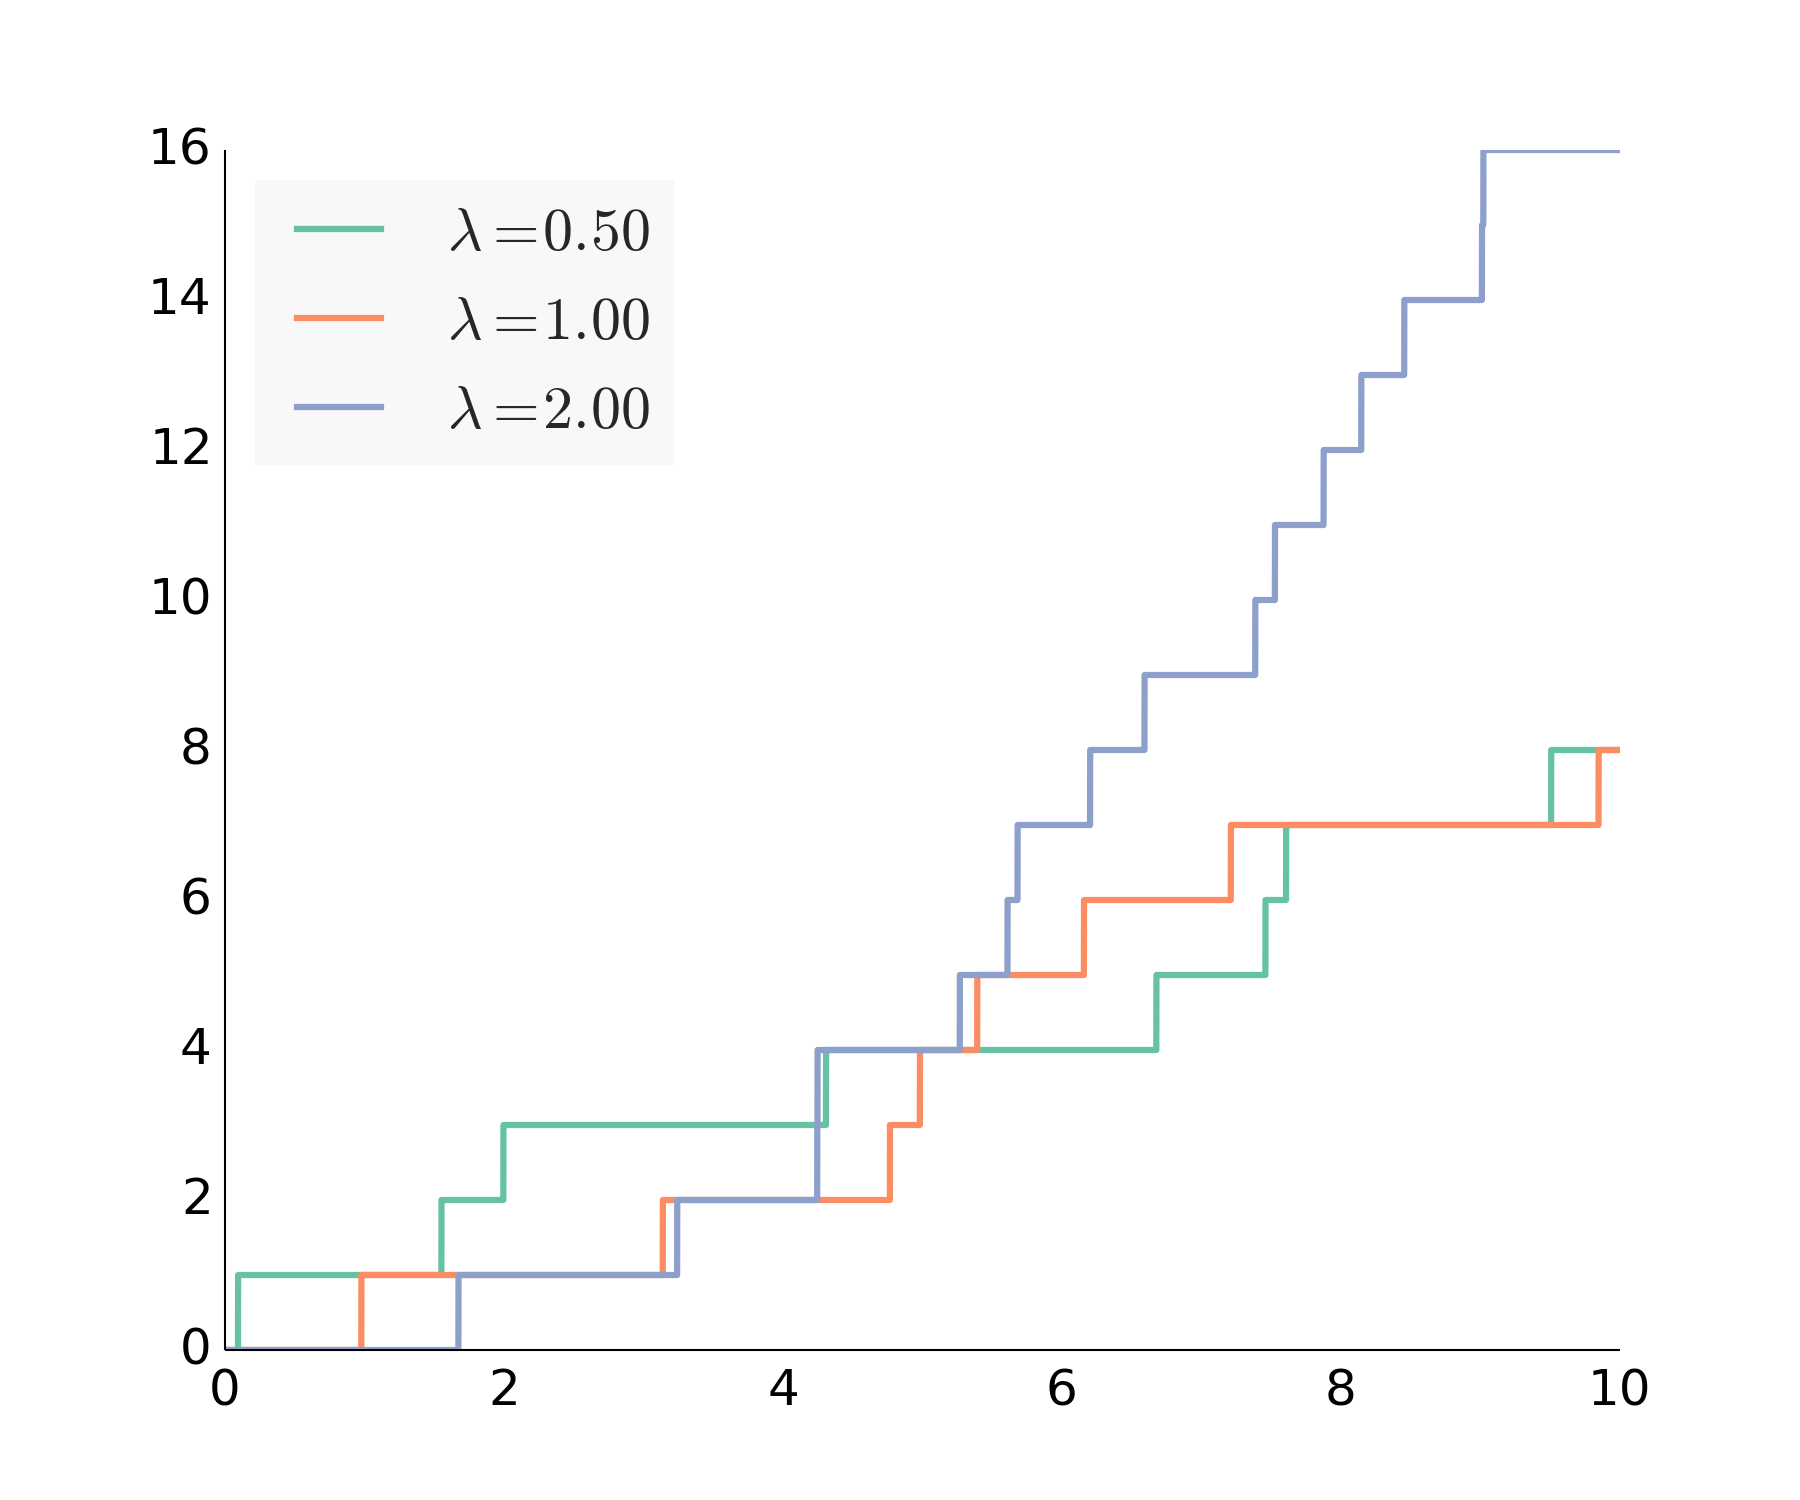
\includegraphics[width=\columnwidth]{figures/figure_2_1.pdf}
\caption[Samples of Poisson Processes.]{Samples of Poisson processes with rates equal to $0.5, 1.0$ and $2.0$.}
\label{fig:poisson_example}
\end{marginfigure}
\par
A doubly stochastic Poisson process, is a process where the rate $\lambda$ is itself a stochastic random variable, usually a function of another stochastic process
$X(t)$. In the case first considered by Snyder, the observations were particle counts of radioactive decay for medical diagnostics. The rate was a function of the 
concentration of the radioactive substance administered to the patient, and by observing particle counts through time onewould like to infer the concentration of 
radioactive substance in the patient's organs. The temporal aspect was relevant because of the fast decay of the radioactive particles. In that case one will have
\begin{subequations}
\begin{equation}
P(N({t+dt})-N(t) = 0 |X(t)) = 1 -\lambda(X(t)) dt + o(dt^2)
\end{equation}
\begin{equation}
P(N({t+dt})-N(t) = 1|X(t)) = \lambda(X(t)) dt + o(dt^2).
\end{equation}
\end{subequations}
The conditional probability of a path $N_{0:t}$ given a path $X_{0:t}$ is then
\begin{equation}
\label{eq:dspp_likelihood}
P(N_{0:t}| X_{0:t}) = \exp\left[ -\int_0^t \lambda(X(s)) ds + \int_0^t \log(\lambda(X(s))) dN(s) \right],
\end{equation}
where I have used the definition of the stochastic integral with respect to a jump process given in \fref{sec:stochastic_proc}.
Defining the jump points $t_i$ as the points where $\lim_{t\downarrow t_i}N(t) \neq \lim_{t\uparrow t_i} N(t)$, one can write the usual formula for the Poisson density of spike times
\[
P(\{t_i\}|X_{0:t}) =   \exp\left[ -\int_0^t \lambda(X(s)) ds \right]\prod_i \lambda(X({t_i})).
\]
Armed with a rate model for the DSPP\marginnote{DSPP: Doubly Stochastic Poisson Process}, one can infer the stimulus history from the count history. The posterior distribution for $X_{0:t}$ is
\begin{equation}
\label{eq:dspp_post}
P(X_{0:t}|N_{0:t}) \propto P(X_{0:t})  \exp\left[ -\int_0^t \lambda(X(s)) ds + \int_0^t \log(\lambda(X(s))) dN(s) \right].
\end{equation}
$P(X_{0:t})$ is a prior distribution over paths of $X(t)$, which in turn are infinite-dimensional objects. This determines the temporal structure of the stimulus, and can be 
tuned to reflect the statistical properties of the stimuli being considered. In practice, it is very hard to compute the full posterior, and for inference purposes, one generally
deals with a  discretised version of the path.\par

Discretising $X_{0:t}$ one can treat the problem of inferring the paths as a multidimensional estimation problem. The simplest way to estimate $X_{0:t}$ is maximum 
likelihood\marginnote{ML = maximum likelihood} whereby one maximises the likelihood given in \fref{eq:dspp_likelihood}. The function given by \fref{eq:dspp_likelihood}
is called a likelihood for $X_{0:t}$ since it does not define a probability density for it. Further, one can incorporate prior beliefs about 
the structure of $X(s)$ by using the full posterior given in \fref{eq:dspp_post}. Taking the value of $X_{0:t}$ that maximises the posterior probability yields the so-called 
\emph{Maximum a Posteriori} estimator.\marginnote{MAP = maximum a posteriori} The full Bayesian approach would be to take the posterior mean as an estimate for 
$X_{0:t}$, that is one takes the mean of the distribution given in \fref{eq:dspp_post} as our estimator. This is usually very hard to compute and has to be done through 
sampling methods.\footnote{For an extensive review of this so-called \emph{decoding} problem see \mycitep{Ahmadian2011,Pillow2011}.}
\par

What if one want to estimate the value of $X(t)$ given $N_{0:t}$ in an online fashion? This corresponds to estimating the marginal probability of $X(t)$ according to
\fref{eq:dspp_post}.
We can derive the results of Snyder informally as follows. Using the same notation as in the Kalman case one has
\[
P(x,t+dt) =\frac{ P\left(X(t+dt)\middle|N_{0:t}\right)P\left(N(t+dt)\middle|X(t+dt)\right)}{P(N(t+dt))}.
\]
When unobserved the distribution of $X$ evolves according to \fref{eq:kolmogorov_fw}. So for infinitesimal $dt$ one can write 
\[
P(X(t+dt)|N_{0:t}) = P(x,t) + \mathcal{A}^\dagger P(x,t) dt.
\]
Furthermore, one can write the quotient of terms dependent on $N(t+dt)$ out as a function of $dN(t)$, leading to
\[
\frac{P(N(t+dt)|X(t+dt),N_{0:t})}{P(N(t+dt))} = (1-dN(t))\frac{1-\lambda(X(t))dt}{1-\hat{\lambda}dt} + dN(t)\frac{\lambda(X(t))}{\hat{\lambda}},
\]
where $\hat{\lambda} = \int dx P(x,t) \lambda(x)$. Expanding and discarding terms of order $dt^2$ and $dN(t)dt$, yields
\[
\frac{P(N(t+dt)|X(t+dt),N_{0:t})}{P(N(t+dt))} = 1-dN(t) -\lambda(X(t))dt +\hat{\lambda}dt +dN(t)\frac{\lambda(X(t))}{\hat{\lambda}},
\]
which rearranging terms, can be written as
\[
\frac{P(N(t+dt)|X(t+dt),N_{0:t})}{P(N(t+dt))} = 1 + \left(\lambda(X(t))-\hat{\lambda}\right)\hat{\lambda}^{-1}\left(dN(t)-\hat{\lambda} dt\right).
\]
Inserting this into the relation above gives
\[
P(x,t+dt) = P(x,t) +\mathcal{A}^\dagger P(x,t) dt + P(x,t)\left(\lambda(x)-\hat{\lambda}\right)\hat{\lambda}^{-1}\left(dN(t)-\hat{\lambda} dt\right),
\]
or, writing it as a stochastic PDE,
\begin{equation}
\label{eq:snyder_uni}
d_t P(x,t) = \mathcal{A}^\dagger P(x,t) dt + P(x,t)\left(\lambda(x)-\hat{\lambda}\right)\hat{\lambda}^{-1}\left(dN(t)-\hat{\lambda} dt\right).
\end{equation}
Note the striking similarity with \fref{eq:kushner}, namely the observations only influence the posterior through an innovation process, here given by $dN(t)-\hat{\lambda}dt$. Furthermore, the inverse rate is equivalent to the inverse variance, since the variance of a Poisson process is precisely its rate $\lambda(x)$. This equation was first derived by Donald Snyder in 1972.\mycite{Snyder1972}
\par
Clearly the derivation above is not mathematically sound. More care is needed when taking limits with $dt\to 0$, namely I have ignored the terms of order $dN(t) dt$ 
in \fref{eq:snyder_uni}. This can be shown to be rigorous, but is beyond the scope of this thesis.\footnote{See \mycitep{privault2014} for a full introduction to the stochastic
calculus of jump processes.} The full derivation by Snyder first finds an expression for the 
characteristic function of the posterior distribution and then derives a stochastic PDE for the characteristic function. This is then Fourier-transformed to yield 
\fref{eq:snyder_uni}.

\subsection{Multiple Spike Trains}

\Fref{eq:snyder_uni} is readily extended to multiple point processes, as long as they are independent. Given a population of point processes $N^i(t)$, $i\in [1,M]$, one will simply have, following the same derivation
\begin{equation}
\label{eq:snyder_multi}
d_t P(x,t) = \mathcal{A}^\dagger P(x,t) dt + P(x,t)\sum_i\left(\lambda_i(x)-\hat{\lambda}_i\right)\hat{\lambda}_i^{-1}\left(dN^i(t)-\hat{\lambda}_i dt\right).
\end{equation}
Again, this can be be compared with a multidimensional observation process in the Kalman case by noting that one can rewrite it as
\begin{equation}
\nonumber
d_t P(x,t) = \mathcal{A}^\dagger P(x,t) dt + P(x,t)\left(\boldsymbol{\lambda}(x)-\hat{\boldsymbol{\lambda}}\right)^\top Diag(\hat{\boldsymbol{\lambda}})^{-1}\left(d\boldsymbol{N}(t)-\hat{\boldsymbol{\lambda}} dt\right).
\end{equation}
I have used the notation $\boldsymbol{\lambda}(x) = (\lambda_1(x),\lambda_2(x),\ldots)^\top, d\boldsymbol{N}(t) = (dN^1(t), dN^2(t),\ldots)^\top$ and so forth. Note that, taking the
vector counting process $\boldsymbol{N}(t)$, its covariance will be $Diag(\hat{\boldsymbol{\lambda}})$, and the equation corresponds precisely to \fref{eq:kushner}.

\section{Fast Population Coding and Dense Tuning Functions}

\label{sec:fast_coding}

A similar filtering framework was proposed in the computational neuroscience community as well.\mycite{Huys2007} The main question being asked was how one can extend the 
framework of population coding, which usually relied on cumulative rates, to coding in a short-time regime. Filtering from spike trains has also been of central importance to the study of 
Brain-Computer-Interfaces, where one tries to decode intended movements or actions from the activity of neurons in the brain.\mycite{Ergun2007} One issue that is central in the 
approach of \mycitet{Huys2007} is the assumption that the population firing rate is independent of the stimulus. I will first extend \fref{eq:dspp_likelihood} to multiple independent Poisson 
processes. This yields
\begin{equation}
\label{eq:dspp_multi_likelihood}
P(\{N^i_{0:t}\}|X_{0:t}) = \exp\left[\sum_i \int \log(\lambda_i(X(s)))dN^i(s) -\int \lambda_i(X(s))ds\right].
\end{equation}
If the tuning functions are distributed such that $\sum_i\lambda_i(X) = C$, irregardless of $X$, this can be simplified substantially. This is the same as saying that the process 
$N(t) = \sum_i N^i(t)$ is a homogeneous Poisson process with rate $C$.
One will then have
\begin{equation}
P(\{N^i_{0:t}\}|X_{0:t}) \propto \prod_i \exp\left[\sum_i \int \log(\lambda_i(X(s))) dN^i(s)\right].
\end{equation}
The integral with respect to $dN^i(s)$ will only yield non-zero terms where $N^i(t)$ is discontinuous, therefore the resulting term will be simply a product of the rates of the neurons at the times they spiked. Let us denote the set of spikes emitted by the population by $\boldsymbol{S}(t) = \{(n_i,t_i)\}_{i=1}^{N(t)}$, where $n_i$ denotes the identitiy of the $i$-th neuron to spike and $t_i$ denotes its spike time. One can then write
\begin{equation}
P(\{N^i_{0:t}\}|X_{0:t}) \propto \prod_{\boldsymbol{S(t)}} \lambda_{n_s}(X(t_s)).
\end{equation}
Furthermore, assume that the the tuning functions $\lambda_i$ are unnormalized Gaussians of the form
\begin{equation}
\label{eq:dense_poiss_gauss_tf}
\lambda_i(x) = \phi \exp\left[-\frac{1}{2} (x-\theta_i)^\top \covar^\dagger (x-\theta_i)\right],
\end{equation}
where I have used the pseudoinverse $\covar^\dagger$ to allow for the tuning functions to be degenerate Gaussian distributions. This poses no problem, as the prior 
over $X(t)$ will be chosen to be Gaussian, leading to a Gaussian posterior when multiplied by $\lambda_i/\hat{\lambda}_i$.
Furthermore the marginal rate of a spike being fired $\hat{\lambda}_i = \boldsymbol{E}_X\left[\lambda_i(x)\right]$ is also 
defined. One must note that $\lambda_i$ does not define a distribution over the stimulus space but a rate of arrival of observations. The Gaussian updates are, however 
the same.\par

I can now treat the problem similarly to the Kalman filter problem, but one needs to take into account the fact that instead of arriving continuously, observations are coming in at random 
times. Consider the same process as before given by the SDE
\[
dX(t) = AX(t) dt + H^{1/2} dW(t).
\]
In the absence of observations the Gaussian distribution will evolve as
\begin{subequations}
\label{eq:free_ou_moments}
\begin{equation}
\frac{d\mu}{dt} = A \mu
\end{equation}
and
\begin{equation}
\frac{d\Sigma}{dt} = A\Sigma + \Sigma A^\top + H.
\end{equation}
\end{subequations}
Therefore, the posterior distribution over $X(t)$ between observations is given by $\mathcal{N}(\mu(t),\Sigma(t))$.
If a neuron with tuning centre $\theta_i$ spikes at time $t$, the posterior density will be updated by
\[
P(X(t)|\textrm{spike}) =\frac{\lambda(X(t)) \mathcal{N}(\mu(t),\Sigma(t))}{\hat{\lambda}}.
\]
Completing squares in the exponents, one obtains for the posterior mean
\begin{subequations}
\label{eq:gaussian_updates}
\begin{eqnarray*}
\mu(t) =&  \left(\Sigma(t^-)^{-1} + \covar^\dagger\right)^{-1} \left(\Sigma(t^-)^{-1} \mu(t^-) + \covar^\dagger \theta_i\right)\\
=&\mu(t^-) -\left(\Sigma(t^-)^{-1} + \covar^\dagger\right)^{-1}\left(\Sigma(t^-)^{-1} + \covar^\dagger\right)\mu(t^-)\\
+&\left(\Sigma(t^-)^{-1} + \covar^\dagger\right)^{-1} \left(\Sigma(t^-)^{-1} \mu(t^-) + \covar^\dagger \theta_i\right),
\end{eqnarray*}
and finally
\begin{equation}
\mu(t) = \mu(t^-) + \Sigma(t)^{-1} \covar^\dagger\left(\theta_i - \mu(t^-)\right).
\end{equation}
For the covariance one has
\begin{eqnarray*}
\Sigma(t) =& \left(\Sigma(t^-)+\covar^\dagger\right)^{-1}\\
=& \Sigma(t^-) -\Sigma(t^-)\left(\Sigma(t^-)+\covar^\dagger\right) \left(\Sigma(t^-)+\covar^\dagger\right)^{-1}+\left(\Sigma(t^-)+\covar^\dagger\right)^{-1},
\end{eqnarray*}
yielding
\begin{equation}
\Sigma(t) = \Sigma(t^-) - \Sigma(t^-) \covar^\dagger \Sigma(t^-) \left(I+\covar^\dagger \Sigma(t^-)\right)^{-1}.
\end{equation}\marginnote{These updates can be simplified if the tuning matrix $E$ is invertible.}
\end{subequations}
These equations can be condensed into SDE's for the posterior mean and covariance very simply. The mean will be given by
\begin{subequations}
\label{eq:filtering_sdes}
\begin{equation}
d\mu(t) = A\mu(t) dt + \sum_i dN^i(t) \left[\Sigma(t^-)\left(I+\covar^\dagger \Sigma(t^-)\right)^{-1} \covar^\dagger\left(\theta_i - \mu(t^-)\right)\right]
\end{equation}
and the covariance by
\begin{equation}
\label{eq:filtering_sde_sigma}
d\Sigma(t) = (A\Sigma(t) + \Sigma(t) A^\top+H)dt + dN(t) \left[\Sigma(t^-) \covar^\dagger \Sigma(t^-) \left(I+\covar^\dagger \Sigma(t^-)\right)^{-1}\right].
\end{equation}
\end{subequations}
These SDE's define processes that are continuous from the right and have a limit from the left. They are often called C\`adl\`ag processes in the stochastic literature, 
from the french phrase \emph{continue \`a droite, limite \`a gauche}. The evolution of the posterior variance only depends on the total spike count process 
$N(t)$, which will be fundamental for the future analysis.
\par

As I mentioned before, the covariance of the tuning functions does not need to be invertible. Note that as long as $\Sigma(t)^{-1} + \covar^\dagger$ is invertible, the 
filtering 
equations are always well-defined. This can be ensured by requiring that $E$ be positive semidefinite. Since $\Sigma(t)$ is positive definite, as it 
is a covariance matrix, $\Sigma(t)^{-1}+\covar^\dagger$ will also be positive definite.
\par

Most of the analytic work in this thesis is done on the filtering problem given by \fref{eq:filtering_sdes}. The fact that the total frequency of observations is independent of 
the system's state along with the homogeneous nature of the population of processes leads to a number of simplifications when evaluating the
Mean-Squared-Error\marginnote{Mean-Squared-Error $\equiv$ MSE} of the estimator $\mu(t)$. More specifically, since $\mu(t)$ is the posteriori mean estimator, its MSE is 
given by the average posterior variance.\footnote{This will be shown in the beginning of \fref{chap:mse}.}
The filtering scheme described in this section and some of the results of \fref{chap:mse} are illustrated in \fref{fig:matern_coding}.
\begin{figure}
\label{fig:matern_coding}
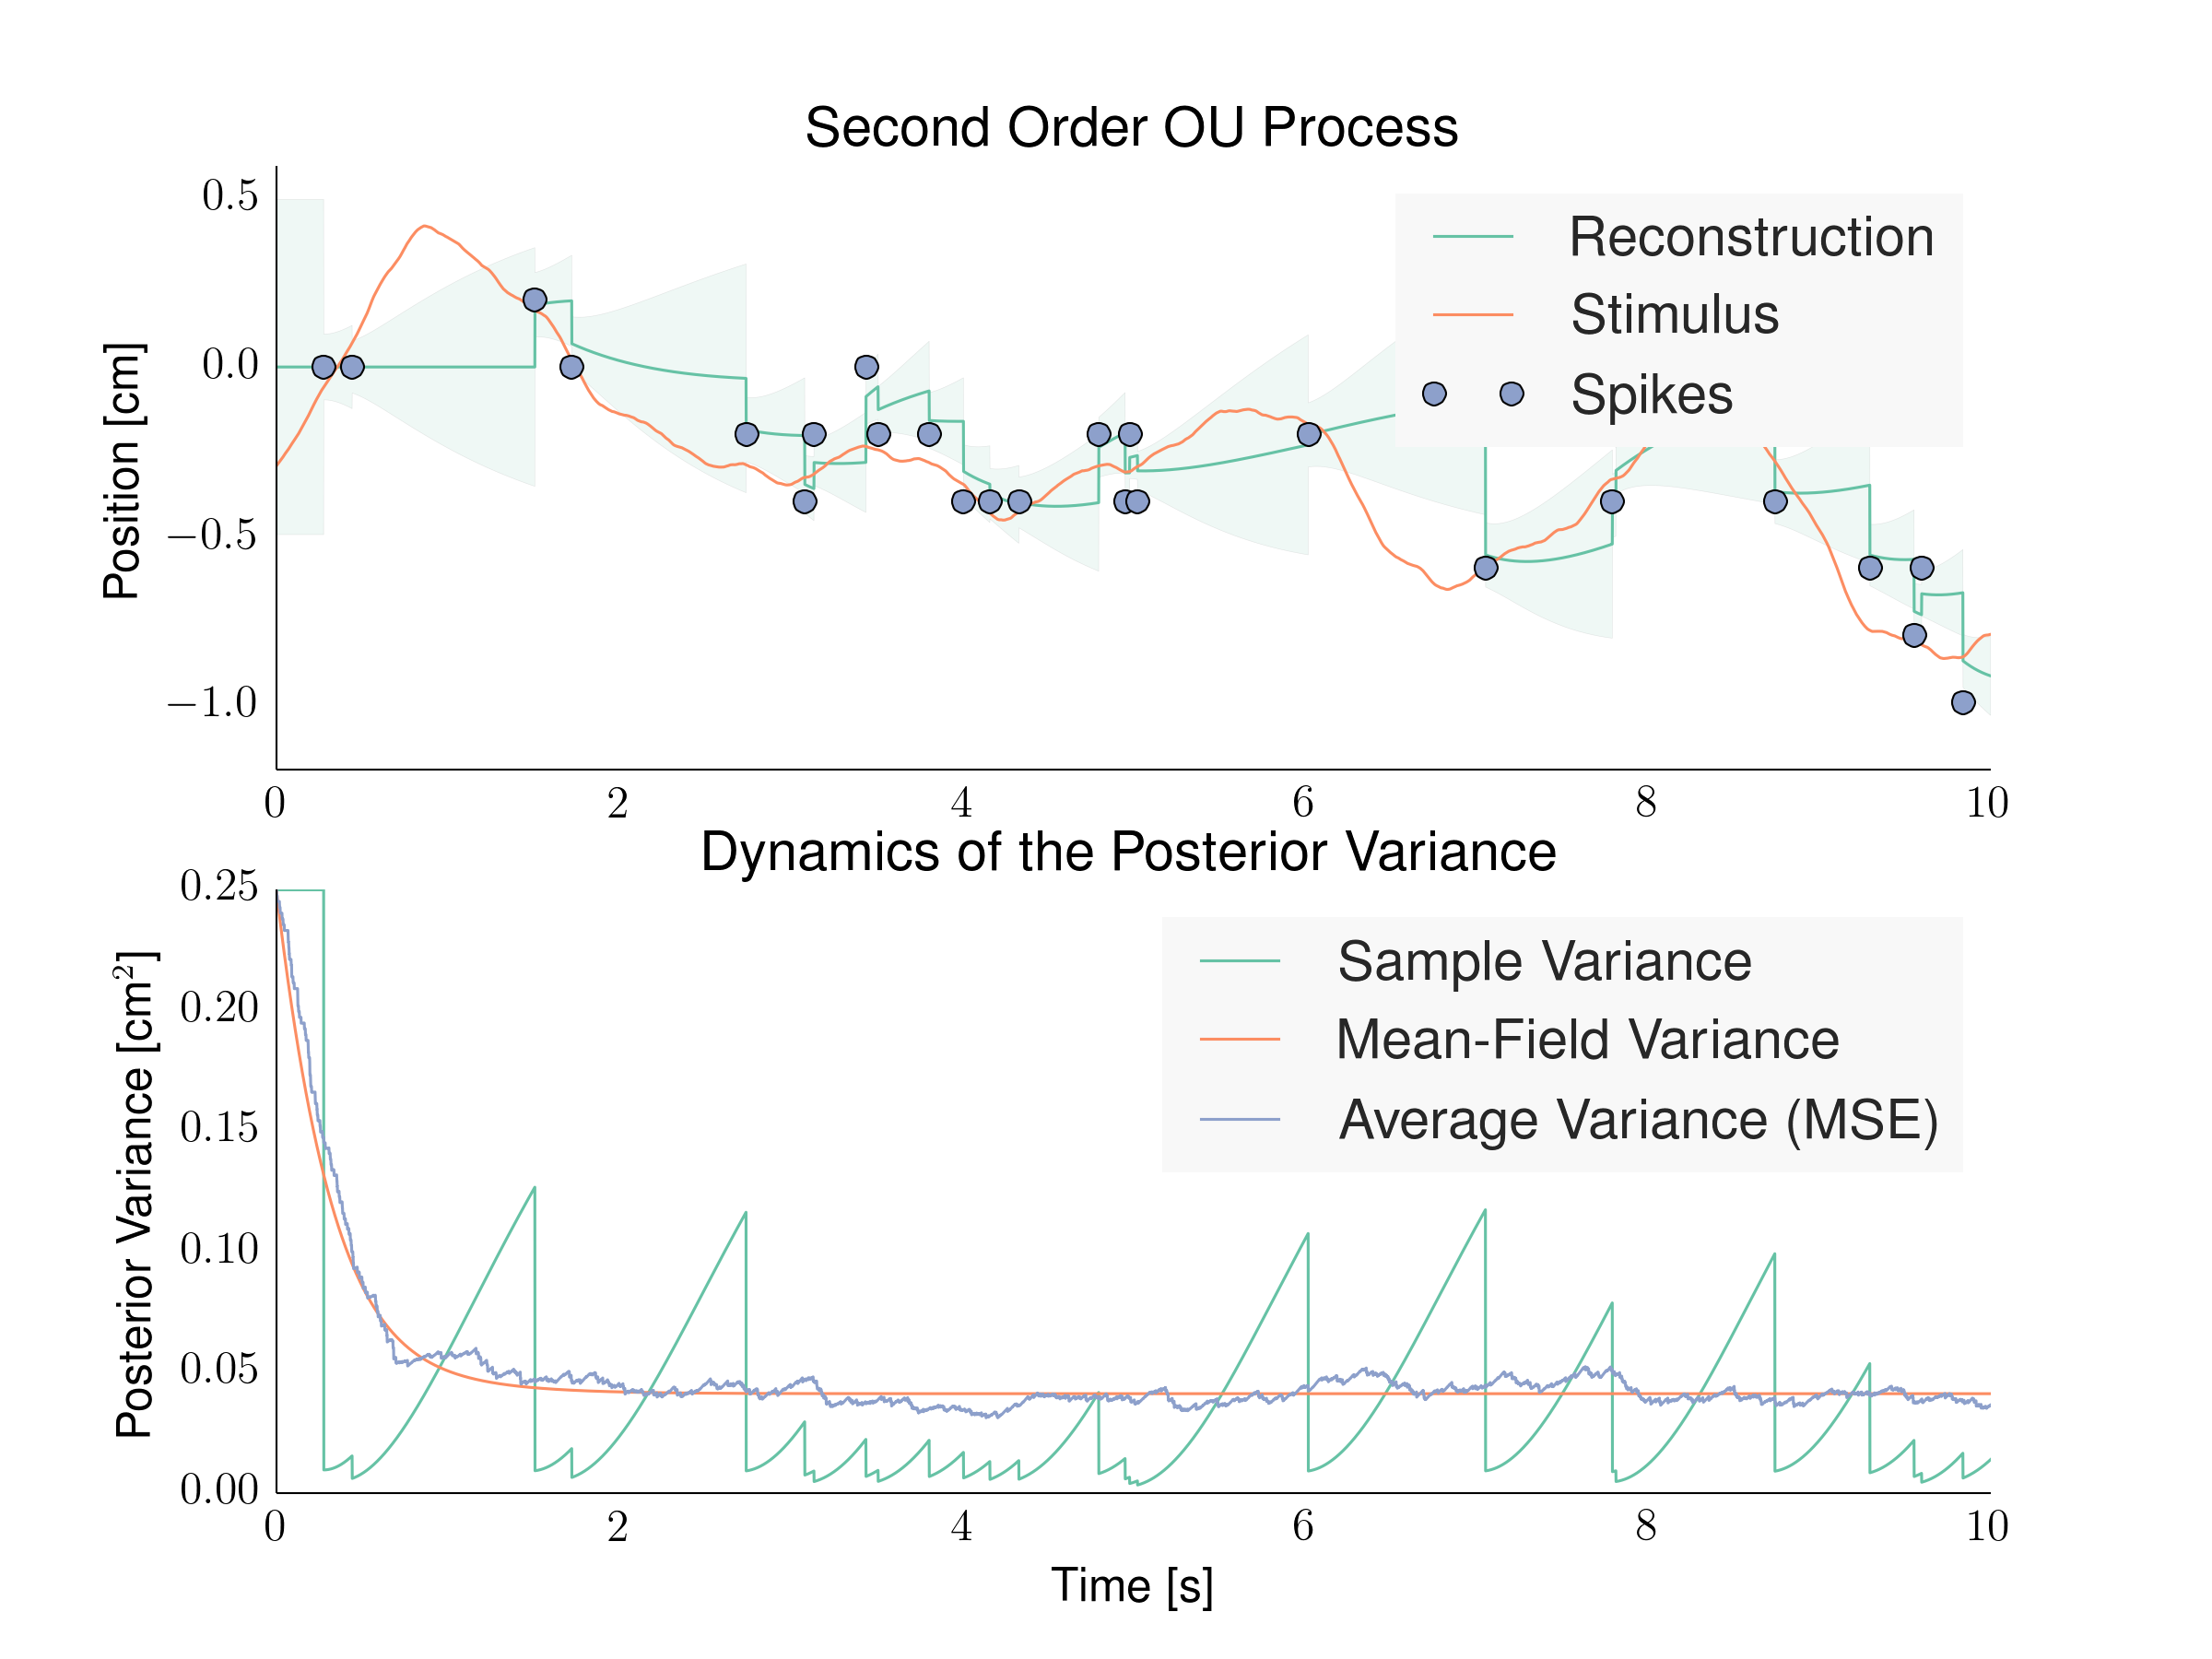
\includegraphics[width=\columnwidth]{figures/figure_2_2.pdf}
\caption[Online decoding of a spike train.]{The general filtering framework: the unobserved process we are trying to estimate is shown as the solid red line, while the observed spikes are
shown as red dots, aligned by the preferred stimulus of the firing neurons. The posterior mean estimate is given by the dotted blue line, while the light red shading
gives the confidence interval of one standard deviation. Note the discontinuous jumps in the mean and covariance at the times of spikes. The lower figure shows the
average posterior variance over all possible spike trains given a stimulus distribution. Note that the mean-field approximation provides a very good account of the
evolution of the average. These results will be further discussed in \fref{chap:mse}.}
\end{figure}

I will now turn to filtering from Point processes when the dense coding assumption does not hold.

\section{Methods for General Filtering of Point Processes}

If nothing else is known about the process at hand, one is forced to work directly with \fref{eq:snyder_multi}. In principle one could discretise the state space and try to 
solve the Partial Differential Equation\marginnote{Partial Differential Equation $\equiv$ PDE} recursively as the observations come in. In practice, however, 
the right hand side \fref{eq:snyder_multi} also contains averages over $P(x,t)$, leading to additional complications on every integration step. One way to circumvent this 
particular problem is to work with unnormalized probabilities. The Zakai equation\mycite{Zakai1969} is a modified version of the Kushner equation which propagates 
unnormalized probabilities. For a stochastic process $X(t)$ observed through another process $Y(t)$ as given in \fref{sec:kalman}, one can define $\rho(x,t)$ as a solution to
\begin{equation}
\label{eq:zakai}
d_t\rho(x,t) = \mathcal{A}^\dagger \rho(x,t) dt+ \rho(x,t) x^\top C^\top D dY(t),
\end{equation}
with $\rho(x,0) = P_0(x)$. It can then be shown that $P(x,t) = \rho(x,t)/\int dx \rho(x,t)$.
Any solution to the Zakai equation will yield a solution to the corresponding Kushner equation when normalised.
Note that, while the Kushner equation was a stochastic partial integro-differential equation, since the left hand side involved averages over $P(x,t)$, the Zakai equation is 
a simpler linear stochastic partial differential equation and given a realisation of the observation process can be solved by standard PDE methods.
%Furthermore, the Zakai equation allows for a closed form solution in terms of path integrals.
\par
I will present a similar framework for the Snyder equation \ref{eq:snyder_uni}. Again taking the notation $P(x,t) = \rho(x,t) / \int dx \rho(x,t)$ one finds that the 
unnormalised posterior distribution $\rho(x,t)$ of a stochastic process with generator $\mathcal{A}$ observed through a doubly stochastic Poisson process with 
rate 
$\lambda(x)$ will obey the stochastic PDE
\begin{equation}
\label{eq:zakai_snyder}
d_t\rho(x,t) = \mathcal{A}^\dagger \rho(x,t) dt -\lambda(x) \rho(x,t) + \left(\lambda(x) -1 \right)\rho(x,t) dN(t).
\end{equation}
Note that any term independent of $x$ can be trivially discarded as it only constitutes a temporal renormalisation of $\rho$. For example, if $\rho^*(x,t)$ is a solution to
\fref{eq:zakai_snyder} with initial condition $\rho(x,0) = g(x)$, then $r(x,t) = \exp\left(-\int_0^t k(s) ds ) \rho^*(x,t)\right)$ is a solution to the stochastic PDE
\[
d_t r(x,t) = \mathcal{A}^\dagger r(x,t) dt -\lambda(x) r(x,t) + \left(\lambda(x) -1 \right) r(x,t) dN(t) -k(t) r(x,t) dt,
\]
with the same initial condition.
This allows one to set a baseline to the expected firing rate in the unnormalised equation. This framework has been used by \mycitep{Bobrowski2009} in
the study of finite state systems observed through doubly stochastic Poisson processes. This work was also extended to static continuous processes by 
Yaeli and Meir.\mycite{Yaeli2010}. I will now discuss the application of these equations to the development of a particle filter for the filtering problems discussed above.


\subsection{Particle Filtering}

The central idea of particle filtering is relatively simple. If one is not given access to the system's state directly, one can just simulate a large number of hypotheses of 
the  system's state and weight each copy according to its agreement with the observations. One can then compute averages over the posterior distribution from the 
weighted samples. Say I have a system with state $X(0)$ initially distributed according to $P_0(x)$, some known transition probability 
\[
W(x,x') \equiv P_{X(t)}\left(x\middle|\,X(t)=x'\right),
\]
and I am given observations of a second process $Y(t)$, with probability density 
\[
\mathcal{L}(y,x) \equiv P_{Y(t)}\left(y\middle|\,X(t)=x\right).
\]
If all the probabilities are known I can implement the filtering  steps numerically,
by taking a sample of $M$ \emph{particles} $\{Z^i(0)\}, i \in [1,\ldots,M]$ from $P_0(x)$, and associating a weight to each of those 
particles $w^i(0)= 1$. Then for each 
particle $Z^i$ I sample the state of that particle at the following instant through the transition probability 
\[
P_{Z^i(t)}(z|Z^i(t-dt)) = W(z,Z^i(t-dt))
\]
and reweigh it through the likelihood
of $Y(t)$, yielding 
\[
w^i(t) = w^i(t-dt) \mathcal{L}(Y(t),Z^i(t)).
\]
The approximate density $Q(x,t) = \sum_i w^i(t)\delta(Z^i(t) - x)/\sum_i w^i(t)$, then gives an 
approximation of the
posterior density $P(x,t)$ and averages can be computed by simply aggregating over the particles, giving
\[
\int dx\, P(x,t) g(x)  \approx \int dx\, Q(x,t) g(x)  = \frac{1}{\sum_i w^i(t) }\sum_i w^i(t) g(Z^i(t)).
\]
These methods are often called Sequential Monte Carlo\marginnote{SMC: Sequential Monte Carlo} methods, since they consist of sequentially sampling the 
state of the system in a way similar to a Monte Carlo Markov Chain.
\par

The description above barely scratched the surface of what is achievable and what are the problems of particle filters, and I will not dive too deeply into the theory of
them, but one point should be made. Though the sampling procedure described above in principle yields an estimate of the true posterior distribution, a lot can
go wrong when implementing it with a finite number of particles. One issue that plagues many such filters is the issue of weight depletion. Weight depletion refers
to the situation where all but a few particles have very low weights, representing state paths which are incompatible with the observations. This can lead the particle
filter to waste resources estimating the density of regions which don't contribute to the posterior averages, and therefore yielding very poor estimates of the distribution
in the interesting regions. This led researchers to propose resampling steps in the particle filter. Whenever a certain criterion is met (or after every step in the filter) one 
can resample the particles from the set of existing particles according to their weights, i.e., sample $M$ particles from the set $\{Z^i(t)\}$ with probabilities given by
$p_i = w^i(t)/\sum_i w^i(t)$. After that, all weights are reset to 1 and the procedure continues. This forces
the filter to allocate its particles according to its current estimate of the posterior distribution, preventing weight depletion to some extent. It is not a panacea for these 
issues, however, and even properly resampled filters can often end up with very poor estimates of the posterior distribution.
\par

Another important thing to note, is that it is often not possible to efficiently sample from the transition probabilities of the system. In those cases one can still combine
the particle filter with an importance sampling approach. In that sense, at every step one samples from a simpler distribution $Q(Z^i(t)|Z^i(t-dt))$ and reweighs the 
particles according to 
\[
w^i(t) = w^i(t-dt) \frac{P(Y(t) | Z^i(t)) P(Z^i(t)|Z^i(t-dt))}{Q(Z^i(t)|Z^i(t-dt))}.
\]
This allows for efficient sampling, but it adds another source of
weight depletion. Again, if the sampling transition probabilities do not match the system's transition probabilities, the weights will quickly fall to low values, leading to
poor estimates of the posterior distribution.
\par

Let us consider again the general case of doubly stochastic Point process filtering. Note that in the absence of spikes the posterior evolves according to
\begin{align*}
\frac{\partial P(x,t)}{\partial t} =& \mathcal{A}^\dagger P(x,t) + (\hat{\lambda}(t) - \lambda(x,t) ) P(x,t).
\end{align*}
For linear diffusion processes, this simplifies to
\begin{align}
\label{eq:particle_fokkerplanck}
\frac{\partial P(x,t)}{\partial t} =& -\nabla \cdot \left(Ax P(x,t)\right) + \frac{1}{2}\Tr\left[ H \frac{\partial^2 P(x,t)}{\partial x_i\partial x_j}\right]+ (\hat{\lambda}(t) - \lambda(x,t) ) P(x,t).
\end{align}
I can again define an unnormalised density $\rho(x,t)$ evolving according to
\[
\frac{\partial \rho(x,t)}{\partial t} =-\nabla \cdot \left(Ax P(x,t)\right) + \frac{1}{2}\Tr\left[ H \frac{\partial^2 P(x,t)}{\partial x_i\partial x_j}\right] -\lambda(x,t) \rho(x,t),
\]
for which the normalised density $\rho(x,t) / \int dx \rho(x,t)$ satisfies \fref{eq:particle_fokkerplanck}.
It can be shown that the equation above describes the evolution of a drift diffusion process with a death rate of $\lambda(x,t)$. This means that the system evolves
according to the \fref{eq:OU_sde} but there is a transition to a death state with a rate $\lambda(x,t)$.\mycite{Oksendal2003} This allows one to formulate a simple particle 
filter, by propagating the particles with the transition probability of the linear stochastic system and then killing it at a rate $\lambda(Z^i(t),t)$, resampling the particles every
time a particle \emph{dies}. Alternatively one can reweigh the weights according to $1-\lambda(Z^i(t),t)dt$ after every time step, obtaining the same effect.
\par
The particle filtering scheme presented here is very flexible, and is in principle applicable to any kind of stochastic process observed through Poisson spikes. This
approach has also gained traction in the neuroscience community, where particle filters are often used to decode cortical signals from electrophysiological
recordings.\mycite{brockwell2004recursive,Ergun2007} Most BCI application require very low latency though, and often specialised types of Kalman filter are more practical to employ in such settings.\mycite{wu2006bayesian}

\subsection{Assumed Density Filtering}

\label{sec:ADF}

Though the presented framework of DSPP's in dense Gauss-Poisson populations of neurons turns out to be exactly Gaussian, this does not hold generally. For example,
one could have a stimulus-dependent population firing rate, leading to non-Gaussian posteriors. One would
then have to deal with the full extent of the Snyder \fref{eq:snyder_multi}. One way to deal with this is to project the posterior distribution to a Gaussian at every time step, that is, at every time
$t$, one looks at the resulting distribution at the next time step $t+dt$ and approximates it with a Gaussian. To do
so one needs to determine the mean and covariance of the posterior and can then match a Gaussian distribution to those moments. 
\par

This approach is usually called Assumed Density Filtering\marginnote{ADF: Assumed Density Filtering}. Given some variable of interest $x$ and a set of observations of random 
variables $\{Y_1,\ldots, Y_N\}$ distributed as $P_Y(y|x)$, ADF consists of sequentially incorporating the observations and
finding the best approximation to the posterior within a family of distributions. For example, if the true, intractable distribution were $P(x|Y_1,\ldots,Y_N)$ one
could choose to approximate it by a Gaussian distribution. One would start out with a prior distribution $Q_0(x)$ and sequentially look
for the best Gaussian approximation to the posterior $Q_i(x) P(Y_{i+1}|x)$. This is usually termed filtering even when there is no temporal estimation
involved because of the sequential updates to the posterior.\footnote{For examples of applications, see \mycitep{opper1998,boyen1998,minka2001}.} The best
approximation to the posterior is usually defined as the one minimising the Kullback-Leibler divergence between the full and approximate posterior. In that sense,
given a current approximation $Q_i(x)$ and a new observation $Y_{i+1}$, the update to our approximate posterior would be
\begin{align*}
Q_{i+1} (x) =& \argmin_q KL[Q_i(x) P(Y_{i+1}|x)||q] \\=& \argmin_q \int dx\, Q_i(x) P(Y_{i+1}|x) \log \frac{Q_i(x) P(Y_{i+1}|x)}{q(x)}.
\end{align*}
The KL divergence taken here is the reverse of the KL divergence used in variational inference.\footnote{In variational inference one usually considers
the KL divergence between the approximating and the true distribution given by $KL[q||p] = \int dx q(x) \log\frac{q(x)}{p(x)}$. When $q(x)$ is tractable or allows for
exact integration, this allows for simplifications of the KL-divergence.} It can be shown that if one applies this 
process using a family of exponential distributions as approximating distributions, it will lead
to a moment matching procedure where the moments of the approximating distribution match the ones of the posterior $Q_i(x) P(Y_{i+1}|x)$.\footnote{See \fref{app:moment} for a 
short 
clarification.} If one took $Q(x)$ to be a Gaussian in every step, the procedure would involve evaluating the mean and covariance of the posterior and setting the new distribution to a 
Gaussian with that mean and covariance.
\par

A simple example of a factor leading to a non-Gaussian posterior in the filtering problem described in this chapter is the presence of adaptation in the firing rates. Poisson processes 
are memoryless,
that is, the probability of a spike being fired is independent of the time since the last spike. It is well known, however, that biological neurons do not follow that rule. For example,
there is a clear refractory period in action potential generation, rendering a neuron incapable of firing an action potential for a short period after the firing of an action potential, 
regardless of the stimulation applied. This
refractory period varies from cell type to cell type and between organisms, but is generally around 5 ms. Another very common phenomenon is
spike-frequency-adaptation,\mycite{benda2003} where upon continued stimulation a neuron reduces its frequency from its initial response frequency to a lower frequency.
A simple Poisson process can not account for these phenomena, but it is easy to modify the Poisson model to account for a refractory period or else to include a spike-frequency 
adaptation component as well.
\par

Consider a simple history-dependent Poisson process given by a rate $\lambda(x,t) = \kappa(t) \lambda(x)$, where $\kappa$ itself depends on the
spiking history of the process. Let me take $\kappa$ evolving according to the SDE
\[
d\kappa(t) = \frac{(\phi - \kappa(t))}{\tau} dt - h(\kappa(t)) dN(t), \quad h(\kappa) = \min(\Delta, \kappa),
\]
where $dN(t)$ is the spike train of the neuron.
This will lead to a rate modulation which stabilises at $\phi$ when there are no spikes, and is shifted downwards by $\Delta$ whenever there is a spike, without
venturing below 0. Although the process is now history-dependent, the joint process $\kappa(t),N(t)$ is still Markov, since the dynamics of $\kappa$ itself
is Markovian. This allows one to model a neuron with a refractory period by taking a relaxation time $\tau \approx 5 ms$ or to model a neuron with spike-frequency-adaptation by taking longer relaxation times.\par

The filtering probability for a diffusion process observed through a population of adaptive neurons with rates given by $\lambda^i(x,t) = \kappa^i(t) \lambda^i(x)$ is given by
\begin{equation}
\label{eq:snyder_adf}
d_t P(x,t) = \mathcal{A}^\dagger P(x,t) dt + P(x,t)\sum_i\left(\lambda_i(x,t)-\hat{\lambda}_i(t)\right)\hat{\lambda}_i(t)^{-1}\left(dN^i(t)-\hat{\lambda}_i(t) dt\right),
\end{equation}
which is \fref{eq:snyder_uni} with time-dependant firing rates. One now needs to integrate the set of equations for the rate modulations $\kappa^i(t)$ for every neuron as well, to be 
able to solve the Snyder equation properly.
\par

The ADF approach for this case would work as follows: one starts out with an initial Gaussian distribution $\mathcal{N}(\mu(0),\Sigma(0))$ at $t=0$; then, for every instant $t$ one 
determines the non-Gaussian probability P(x,t+dt) at the next instant $t+dt$ via \fref{eq:snyder_adf}; after that, one finds the mean and covariance of $P(x,t+dt)$, and approximates the 
distribution by a Gaussian with the same mean and covariance and proceeds to the next instant. This can be cast into a set of differential equations and updates governing the
mean and covariance of our approximate posterior.
\par

To obtain the ADF equations for this simple model I need to evaluate the evolution of the mean and covariance of the filtering distribution. I will derive the
necessary equations similarly to the derivation of the differential Chapman-Kolmogorov equation in \mycitep{Gardiner2004}.The average of
a function of $x$ over the posterior distribution evolves as
\begin{align*}
\frac{\partial \boldsymbol{E}_P[f]}{\partial t} = \frac{\partial \int dx f(x) P(x,t)}{\partial t} = \lim_{dt\to 0} \frac{\int dx f(x) \left(P(x,t+dt)-P(x,t)\right)}{dt}.
\end{align*}
In the absence of spikes, the limit can be evaluated, as all terms are of order $dt$, obtaining
\begin{align*}
\frac{\partial \boldsymbol{E}_P[f]}{\partial t} =& \int dx f(x) \left(\mathcal{A}^\dagger P(x,t) + (\hat{\lambda}(t) - \lambda(x,t) ) P(x,t)\right) \\
=&\int dx  P(x,t) \left(\mathcal{A} f(x)+ f(x) (\hat{\lambda}(t) - \lambda(x,t) ) \right).
\end{align*}
This can be readily cast into a form to allow for moment matching of Gaussian distributions. Taking a stochastic process $X(t)$ given by the SDE
\[
dX(t) = A\left(X(t)\right) dt + H\left(X(t)\right)^{1/2} dW(t),
\]
the infinitesimal generator and its adjoint will be given by
\[
\mathcal{A} f = A(x)^\top \nabla f(x) +  \frac{1}{2}\Tr\left[H(x) \frac{\partial^2 f(x)}{\partial x^2}\right],
\]
and
\[
\mathcal{A}^\dagger f = -\nabla \cdot\left(A(x) f(x)\right) + \frac{1}{2}\Tr\left[ \frac{\partial^2 H(x) f(x)}{\partial x^2}\right].
\]
The evolution of the mean and covariance will thus be given by
\begin{subequations}
\begin{equation}
\frac{\partial \mu(t)}{\partial t } = \boldsymbol{E}\left[A(x)\right] + \boldsymbol{E}\left[x \left(\hat{\lambda}(t) -\lambda(x,t)\right)\right],
\end{equation}
\begin{align}
\frac{\partial \Sigma(t)}{\partial t} = &\boldsymbol{E}\left[A(x)(x-\mu(t))^\top\right] + \boldsymbol{E}\left[(x-\mu(t)) A(x)^\top\right] + H(x)\nonumber\\ +&\boldsymbol{E}\left[(x-\mu(t)) (x-\mu(t))^\top \left(\hat{\lambda}(t) -\lambda(x,t)\right)\right].
\end{align}
\end{subequations}
These equations are exact, even if the posterior distribution is not Gaussian. If the posterior is Gaussian, the averages on the right hand side of these equations can be 
written as a function of $\mu(t)$ and $\Sigma(t)$, therefore providing a closed system for the evolution of these variables. The crucial step to perform ADF is to assume that the 
distribution at every
instant is characterised by only its mean and covariance, and is therefore Gaussian. In that case, the averages in the equations can often be performed exactly and 
one can provide an approximate filter to the problem. Note that the derivation is valid for the case of multiple spike trains as well, yielding
\begin{subequations}
\label{eq:adf_gauss_filter}
\begin{equation}
\frac{\partial \mu(t)}{\partial t } = \boldsymbol{E}\left[A(x)\right] + \sum_i\boldsymbol{E}\left[x \left(\hat{\lambda}^i(t) -\lambda^i(x,t)\right)\right],
\end{equation}
\begin{align}
\frac{\partial \Sigma(t)}{\partial t} = &\boldsymbol{E}\left[A(x)(x-\mu(t))^\top\right] + \boldsymbol{E}\left[(x-\mu(t)) A(x)^\top\right] + H(x)\nonumber\\ +&\sum_i\boldsymbol{E}\left[(x-\mu(t)) (x-\mu(t))^\top \left(\hat{\lambda}^i(t) -\lambda^i(x,t)\right)\right].
\end{align}
\end{subequations}\par

In \fref{chap:optimal} I will apply the ADF approach to the general linear stochastic systems considered here as well as a nonlinear stochastic system and compare 
them to the particle filter approach. 
Though the ADF has had considerable success and has spawned a number of new approaches, most notably the expectation propagation (EP)
algorithm,\mycite{opper2000,minka2001} the theoretical guarantees of particle filters have led me to prefer it when estimating the MSE of an approximate filter.

\section{Filtering for General Gaussian Processes}
\label{sec:gp_filtering}
The linear stochastic processes I have considered in this chapter are special cases of Gaussian Processes. A Gaussian Process is a process $X(t)$ such that the 
marginal distribution of the process at a set of times $\{t_1,\ldots,t_M\}$ is always given by a Gaussian distribution. Furthermore, the density of $X(t)$ at said points
is given by
\[
P\left(X(t_1),X(t_2),\ldots,X(t_m)\right) = \mathcal{N}\left((m(t_1),m(t_2),\ldots,m(t_M))^\top, K(t_i,t_j)\right), \textrm{ where } 1\le i\le M, \quad 1\le, j \le M.
\]
The covariance of a GP\marginnote{GP $\equiv$ Gaussian Process} is given by the kernel function $K(s,t)$, which specifies the temporal structure of the process at 
hand. It is straightforward to show that the unobserved Ornstein-Uhlenbeck process
\[
dX(t) = -\gamma X(t) dt + \sigma^{1/2} dW(t),
\]
describes a Gaussian process with zero mean and kernel $K_{OU} (s,t) = \frac{\sigma}{2\gamma} e^{-\frac{|t-s|}{2\gamma}}$.\par

Gaussian Processes have become a very popular method in Machine Learning, as they allow one to specify a distribution of random functions over a
domain.\mycite{Rasmussen2005}
\par

Assume one is trying to estimate a function $f(t)$ drawn from a GP prior with zero mean and kernel $k(s,t)$. If one is given $M$
observations $(t_i,y_i)$ of the value of $f$ at times $t_i$, one can write the marginal distribution of $f(t)$ for any time $t$ by simple manipulation of Gaussian densities.
If the observations are corrupted with Gaussian noise with variance $\alpha^2$, the probability density of the observations is given by
\[
P(y_1,\ldots,y_M) = \mathcal{N} (\boldsymbol{0},K(t_i,t_j)+\alpha^2 \delta_{i,j}), \textrm{ where } 1\le i\le M, \quad 1\le, j \le M.
\]
The joint density of $f(t)$ and the observations is given by
\[
P(f(t),y_1,\ldots,y_M)= \mathcal{N} \left(\boldsymbol{0},\left[\begin{array}{cc} K(t,t) & K(t,t_i)\\K(t,t_j)& K(t_i,t_j)+\alpha^2\delta_{i,j}\end{array}\right]\right).
\]
Let $G_{i,j} = K(t_i,t_j)$, $\boldsymbol{y} = (y_1,\ldots,y_M)^\top$ and $k(t,\{t_i\}) = (K(t,t_1),\ldots,K(t,t_M))^\top$.
The conditional distribution of $f(t)$ given the observations can then written as
\[
P(f(t)|y_1,\ldots,y_M) =\mathcal{N}\left(\hat{f}(t), \Xi(t,t)\right),
\]
where
\begin{subequations}
\begin{equation}
\hat{f}(t) = k(t,\{t_i\})^\top (G + \alpha^2 \boldsymbol{I})^{-1} \boldsymbol{y},
\end{equation}
and
\begin{equation}
\Xi(t,t) =  K(t,t) - k(t,\{t_i\})^\top (G+\alpha^2\boldsymbol{I})^{-1} k(t,\{t_j\})^\top.
\end{equation}
\end{subequations}
As I have shown above, if $t> t_i \forall i, \textrm{ s.t, }1\le i\le M$, these relations can be cast into the form of stochastic differential equations for a number of kernels. The OU kernel 
and its corresponding SDE were shown above, but another example I will refer to is the Matern kernel of order $\nu = 3/2$, given by
\[
K_{Mat}(t,s) = \eta\left(1+\frac{\sqrt{3}|t-s|}{l}\right) e^{-\frac{\sqrt{3}|t-s|}{l}}.
\]
The samples of the kernel correspond to a critically damped stochastic oscillator with a white-noise force being applied to it. Samples from this process can be seen in
\fref{fig:stoch_example}. I have chosen the scaling factor to obtain the same characteristic length as the RBF kernel below. It can be shown that an appropriate limit of
Matern kernels of increasing order will converge to the RBF kernel (see \mycitep{Rasmussen2005}).\par

The approach developed in the beginning of this chapter is very practical as it allows us to use the tools of stochastic dynamics to analyse the expected mean-squared 
error of the optimal filter, but in the general case of GP's this is not possible. In the case of smoother GP's such as the ones given by the RBF kernel
\[
K_{rbf} = \eta\exp\left[-\frac{|t-s|^2}{2 l^2}\right],
\]
the future covariance depends on all past observations, and one can not formulate simple Markov dynamics for the posterior variance. I will develop a theory
for the evolution of the entire posterior kernel 
\[
\Xi(t,s) = \boldsymbol{E}\left[(f(t)-\hat{f}(t))(f(s)-\hat{f}(s))\middle| \boldsymbol{y}\right] 
\]
in the next chapter, which allows one to evaluate the average performance of the optimal filter on a general GP observed through Poisson spikes. The learning
performance of GP regression methods is still an active area of research, and recent efforts using methods from statistical physics of disordered systems have shown
promising advances.\footnote{See \citep{malzahn2005statistical,urry2013}.}





\chapter{Mean-Squared-Error for Point Process Filtering}

\label{chap:MSE}

\epigraph{Well, my theory is that your theory is wrong.}{Fernanda G. P. Susemihl}

In the previous chapter I have introduced filtering methods for stochastic processes observed through Poisson processes. In this chapter I will deal with the issue of how well one
can estimate that process from a set of Poisson processes with a given set of rate functions.\par

If one has an estimate $\hat{X}$ of some stochastic variable $X$ to be estimated , how
can one quantify the error incurred by the estimator? One needs to specify some loss function that assigns a cost to an error $|\hat{X}-X|$. It makes sense to require the loss function to
be increasing and to require the loss of an exact estimate to be zero, but other than that, any loss function could do. Here I will consider results on the squared loss function
\[
L^2(\hat{X},X) = (\hat{X}-X)^2,
\]
leading to the mean-squared-error (MSE) as a measure of the performance of the encoder. This is specially convenient when dealing with Gaussian distributions, as a number of 
analytical  results can be derived. Other possible choice would be the absolute loss, given by
\[
L^1(\hat{X},X) = |\hat{X}-X|.
\]
In other situations, such as classification tasks, other loss functions are useful, but I will restrict myself to the MSE case here.\par

When dealing with stochastic processes, it is usually more convenient to consider the covariance matrix of the process, rather than the squared error, which is given by the
sum of the variances of every coordinate of the process.
Let me then define the mean-squared error matrix as
\[
\boldsymbol{MSE}(\hat{X}) = \boldsymbol{E}\left[ (\hat{X} - X) (\hat{X}-X)^\top\right],
\]
where the expectation is over all possible realisations of $X$ and over the observations leading to the estimator $\hat{X}$. Alternatively one could take the average to be over
multiple realisations of an experiment, or over long time averages of a temporal estimation problem.
To obtain a scalar measure of the estimation error, one can just take the trace of the MSE matrix.
This scalar error will be written as 
\[
MSE = \Tr( \boldsymbol{MSE}) = \boldsymbol{E}\left[ (\hat{X} - X)^\top (\hat{X}-X)\right].
\]
If further one knows that the estimator $\hat{X}$ depends on some 
parameters $\theta$, she could seek out the optimal estimator $\hat{X}^*$ by taking the parameters $\theta^*$ that minimise the MSE
\[
\theta^* = \textrm{argmin}_\theta MSE( \hat{X}(\theta)  ).
\]
Assuming I am estimating $X$ from an observation process $Y$ dependent on $X$, I can write
\begin{equation}
\label{eq:bayes_mse}
MSE( \hat{X}(Y) ) = \int dX dY  (\hat{X}(Y) - X)^\top (\hat{X}(Y)-X) P(X|Y)P(Y).
\end{equation}
Since $P(Y)\ge 0$ for every $Y$, minimising the inner integrand $\int dX (\hat{X}(Y) - X)^\top (\hat{X}(Y)-X) P(X|Y)$ for every $Y$ will lead to a minimum of the full integral. So, minimising the inner integrand with respect to the estimator will lead to
\[
\frac{\partial \int dX (\hat{X}(Y) - X)^\top (\hat{X}(Y)-X) P(X|Y)}{\partial \hat{X}(Y)} = 2 \int dX (\hat{X}(Y) - X) P(X|Y).
\]
Equating the derivative to zero leads to the minimum mean squared-error (MMSE) estimator for $X$, given by
\[
\hat{X}^*(Y) = \int dX\, X\, P(X|Y) = \boldsymbol{E}[X|Y].
\]
The MMSE estimator is often called the Bayes estimator for $X$ given the observations $Y$, since it minimises an expected loss given by \fref{eq:bayes_mse}, which treats
the quantity being estimated as a random variable with a prior probability distribution.
The MMSE estimator, however, can only be exactly computed if the true data generating distribution $P(Y|X)$ along with the true signal distribution $P(X)$ is known, allowing one
to estimate the posterior probability $P(X|Y)$. Furthermore, the Bayes 
estimator involves averaging over the signal space, which can be impractical. A number of techniques can be used to approximate the estimator though, such as Gaussian
processes or neural networks. The optimality of the MMSE estimator is a central result in information theory, and the MMSE estimator is usually taken as the standard to 
estimation.\footnote{Minimising a different loss function or error measure would lead to a different optimal estimator. Minimising the expected absolute loss, for example, 
leads to the posterior median as the optimal estimator.}
\par

However, finding the optimal estimator is not the end of the story. Often the design of sensors and of the experimental process allow one to change the data 
generating distribution $P(Y|X)$. For a simple example, consider a radar gun. Assume it gives a measure of the speed of the considered vehicle corrupted  with 
Gaussian noise with zero mean and standard deviation of $5\,\textrm{km/h}$. Indeed, given a number of measurements of the speed of a 
vehicle,\footnote{Assuming the speed of the vehicle remained unchanged across measurement} the MMSE estimator will be the estimator which minimises the 
expected 
MSE. Regardless of that, however, one can always reduce the MSE by using a radar gun with a smaller noise rate. A superior radar gun which outputs 
measurements with standard deviation of $1\,\textrm{km/h}$ will certainly reduce the MSE further. In most simple cases, however, this reduction is obvious, as one 
simply strives to reduce the noise as much as possible.
\par

The neural case poses an interesting exception though. Considering the Poisson model from the previous chapter, the probability of a spike being fired in a small time 
interval $dt$ conditioned on the stimulus $X$ is given by $\lambda(X)dt$. The probability of a spike being fired averaged over all stimuli $X$ would then be given by
$\hat{\lambda}dt = \int dx\, P(x)\, \lambda(x)dt$. If one tries to increase the precision of the likelihood defined by $\lambda(X)$, for example by reducing the 
width of the tuning function, this will automatically reduce the probability of that neuron firing. Therefore, there is a trade-off between frequency of firing and precision of 
firing, which is not present in the case of additive Gaussian noise. This is illustrated in \fref{fig:neuron_example}, where I show two Poisson neurons with Gaussian tuning functions
and the same preferred stimulus but with different precisions. The upper neuron has a broader tuning function, leading to a higher firing rate, but in turn the spikes are less 
discriminating of the value of the stimulus. The second neuron has a much narrower tuning function, leading to more precise observations of the stimulus, but a much lower
spiking frequency. It is not immediately clear which neuron will allow for a better reconstruction of the underlying stimulus, as the influence of the frequency and the precision
of the spikes would have to be pitted against each other.
\par

\begin{figure*}
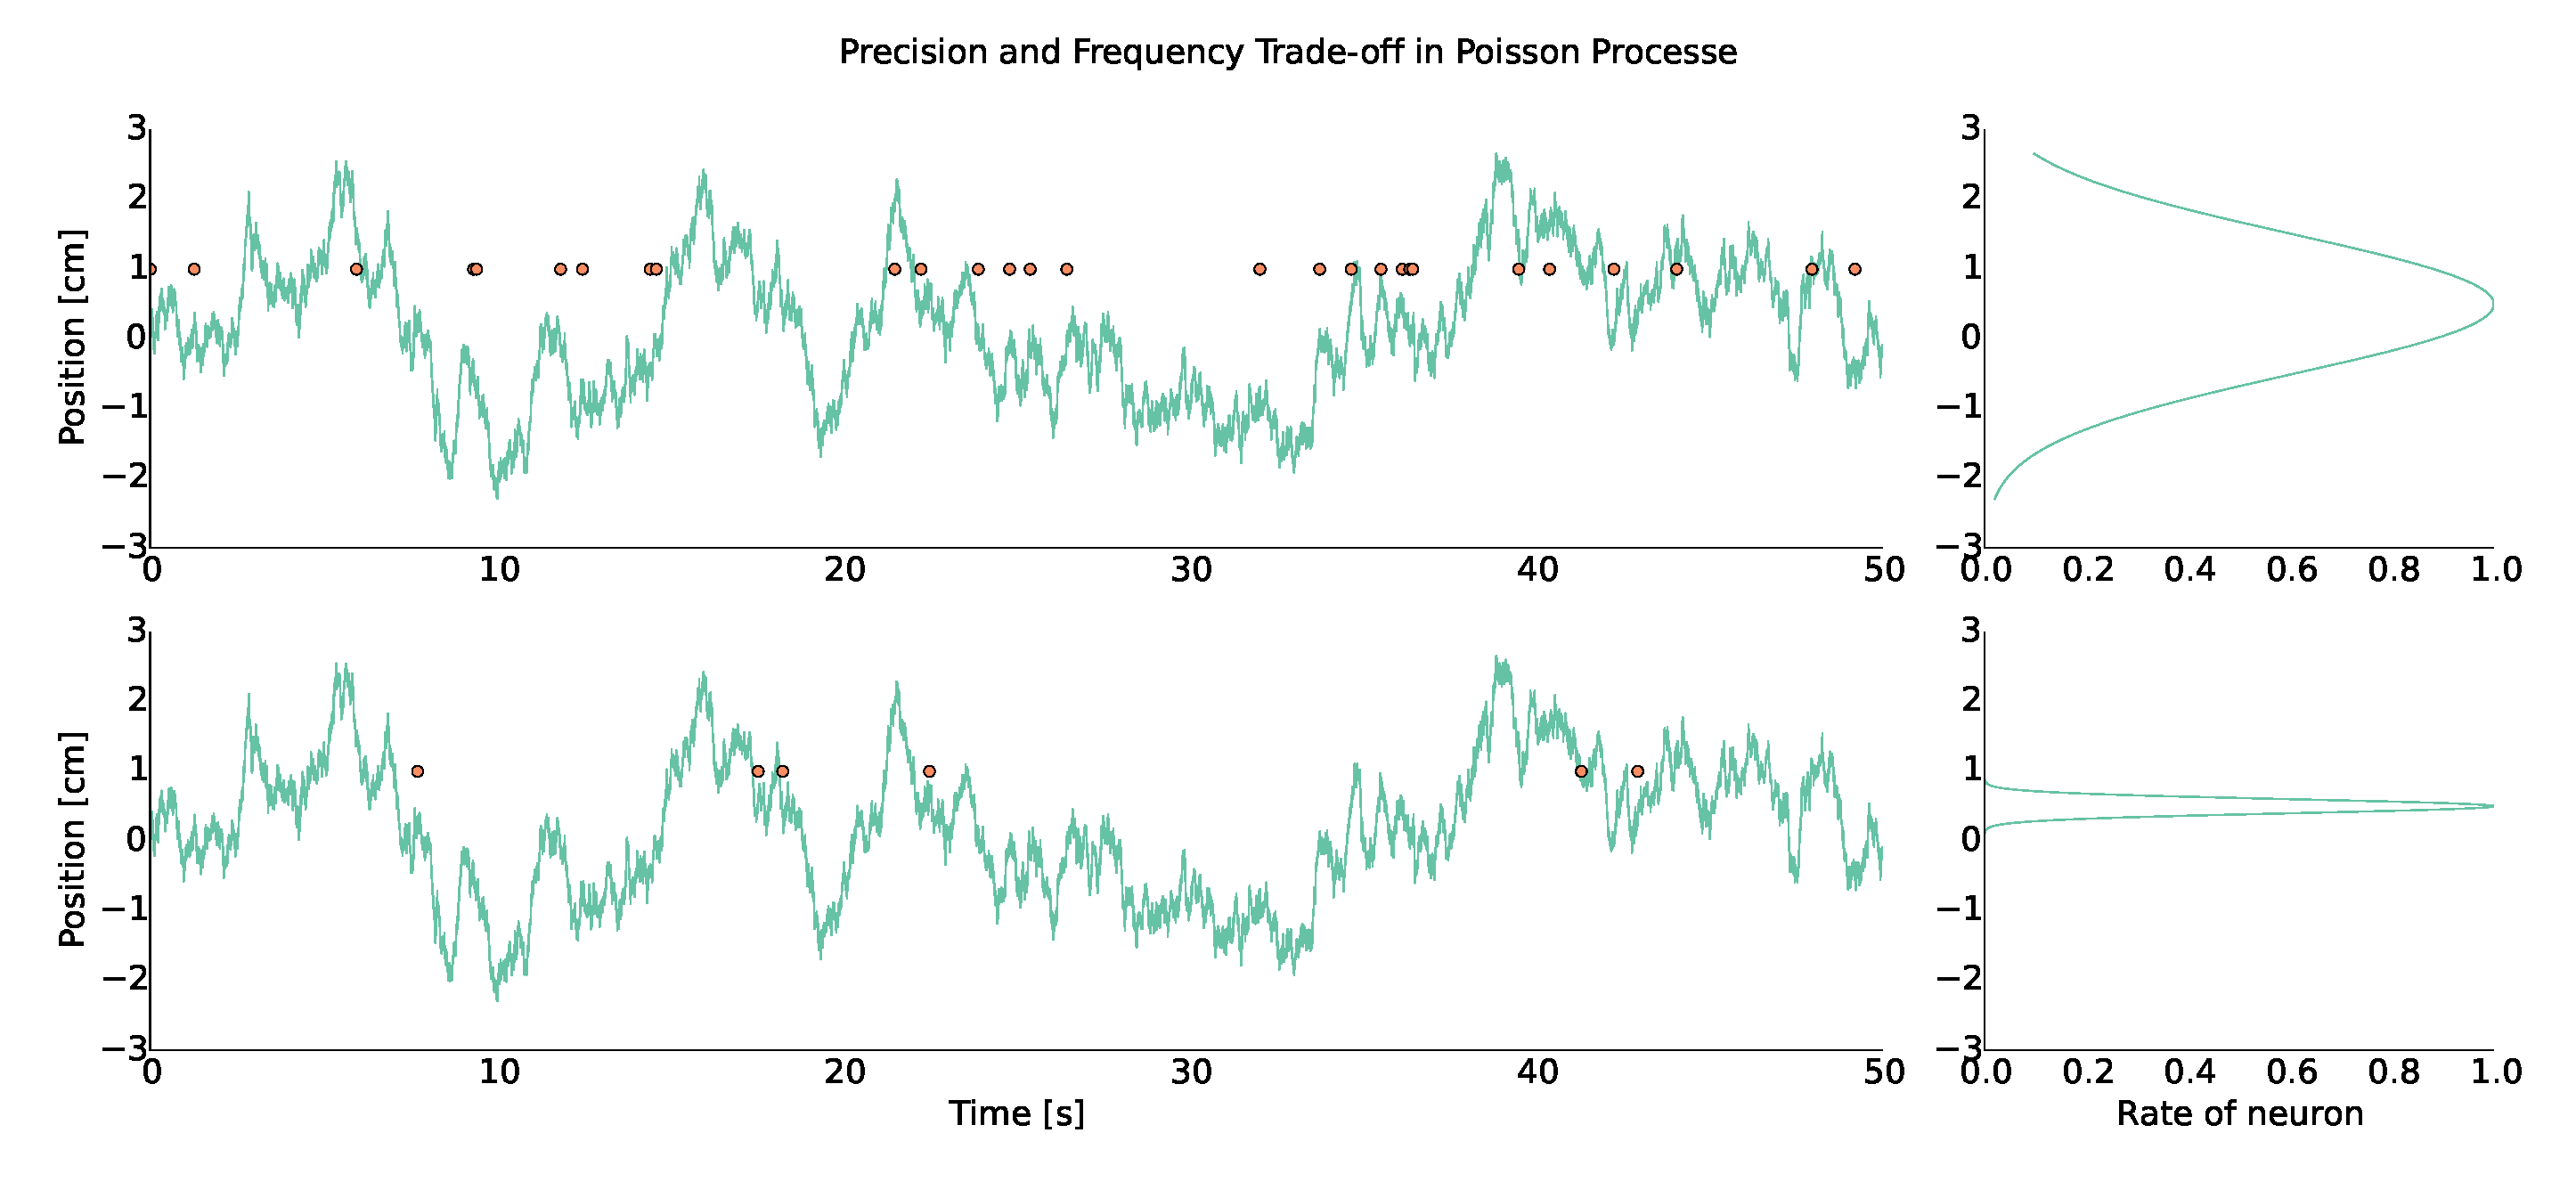
\includegraphics[width=\columnwidth]{figures/figure_3_example.eps}
\caption[Trading off precision and frequency in spike observations.]{The tradeoff between precision and frequency. The upper plot shows the spike train of a single neuron with a Gaussian tuning function with unit width responding to a
stochastic stimulus. There are quite a few spikes but they are fairly unreliable. The lower plot shown a neuron with a Gaussian tuning function with a width of $0.2$. There are
nearly no spikes, but they spike only when the neuron is in a narrow range around the neuron's tuning centre.}
\label{fig:neuron_example}
\end{figure*}

In this chapter I will derive a number of exact and approximate relations for the MSE of the optimal filters described in the previous chapter. I will provide a solution for the stationary distribution of the
posterior variance of the optimal filter for the OU process, showing that this distribution diverges when the average interspike interval is longer than the relaxation time of the variance. I will present a 
number of approximate treatments of limiting cases, for low firing rates and for the diffusion limit of large observation noise. Finally I will provide a treatment of the average posterior
kernel, which allows us to study the MSE of the optimal filter of general Gaussian processes. My goal in this chapter is to develop exact and approximate methods to study the average
MSE performance of the optimal filter of a system observed through a population of doubly stochastic Poisson processes. Armed with that, I will in \fref{chap:optimal} look at the
optimal strategies for these processes to encode the state of system, namely the ones that minimise the MSE.

\section{The MSE for Dense Gaussian DSPP Observations}

In \fref{sec:fast_coding} I have discussed case of dense populations of Gauss-Poisson neurons, first introduced in \mycitep{Huys2007}. 
This framework allows for a number of simplifications. Most importantly, the posterior variance of the filter obeys a SDE with drift and jumps where the jumps occur with
a state-independent rate $\hat{\lambda}$. As I have discussed above, the MMSE estimator gives the optimal estimator for a data-generating distribution $P(Y|X;\covar,\{\theta_i\},\phi)$. 
However, if the response properties of the neural population change (through changes in $\covar$, $\phi$ or the positioning of the tuning functions), the performance of the estimator
will change as well and one can ask which is the encoder that provides the lowest MMSE.
\par

As in \fref{sec:fast_coding}, let the stimulus be a stochastic process $X(t)$, and the observations be spike trains of a dense population of Gauss-Poisson neurons
$\boldsymbol{N}(t) = (N^1(t),\ldots, N^M(t))^\top$. Writing $\boldsymbol{N}_{0:t} = \{\boldsymbol{N}(v), \forall v \in [0,t]\}$, the posterior distribution is
\[
P(X(t)|\boldsymbol{N}_{0:t}) = \mathcal{N} \left(\mu(t;\boldsymbol{N}_{0:t}),\Sigma(t;\boldsymbol{N}_{0:t})\right),
\]
where $\mu(t;\boldsymbol{N}_{0:t})$ and $\Sigma(t;\boldsymbol{N}_{0:t})$ are solutions to \fref{eq:filtering_sdes}.
% with initial conditions $\mu(0) = \mu_0$ and $\Sigma(0)= \Sigma_0$.
The MMSE matrix can be written as
\[
\boldsymbol{MMSE}(t;\{\theta_i\},\covar) = \boldsymbol{E}_{X(t),\boldsymbol{N}_{0:t}}\left[\left(X(t) -\mu(t;\boldsymbol{N}_{0:t})\right)\left(X(t) - \mu(t;\boldsymbol{N}_{0:t})\right)^\top\right]\equiv \epsilon(t).
\]
I am interested in the ensemble average over all possible realisations of both the signal as the observation processes.\par

Throughout this chapter, I assume that the posterior distribution used to evaluate the posterior mean estimator is the same distribution as the one that is generating the observations
$\boldsymbol{N}_{0:t}$. This is called the matched situation. If complete information about the distribution $P(\boldsymbol{N}_{0:t}|X(t))$ was unavailable, one would be forced to work
with an approximate posterior. In the matched case, however, I can simplify the expression for $\epsilon(t)$. Writing out the expectation over $X$ and $\boldsymbol{N}$ gives
\[
\epsilon(t) = \int d\mu\left(X(t)\right) \int d\mu(\boldsymbol{N}_{[0:t]}) \left(X(t) - \mu(t;\boldsymbol{N}_{0:t})\right)\left(X(t) - \mu(t;\boldsymbol{N}_{0:t})\right)^\top P(X| \boldsymbol{N}_{0:t}) P(\boldsymbol{N}_{0:t}).
\]
The average over $P(X|\boldsymbol{N}_{[0:t]})$ will just yield the posterior variance $\Sigma(\boldsymbol{N}_{0:t})$, leading to
\begin{equation}
\label{eq:eps_sigma}
\epsilon(t) = \boldsymbol{E}\left[\Sigma(\boldsymbol{N}_{0:t})\right] = \boldsymbol{E}\left[\Sigma(N_{0:t})\right],
\end{equation}
where in the last step I have used that the posterior variance is only a function of the population spike count $N_{0:t} = \sum_i N^i_{0:t}$ and not of the full spike train $\boldsymbol{N}_{0:t} = \left(N^1_{0:t}, N^2_{0:t}, \ldots\right)^\top$. This makes it much simpler to treat the averages, but they still remain intractable. To get a sense of the problem, for every possible spike count, one would have to average over all possible spike times for those spikes, considering the evolution of $\Sigma$ from its initial value according to the dynamics given in \fref{eq:filtering_sde_sigma}, and then average over all possible spike counts. This has been done for the case of static stimuli in \mycitep{Yaeli2010}. When the stimulus is static, the averages are simplified by the fact that the variance does not change between spikes. The posterior variance is given by
\[
\Sigma(t) = \left(\Sigma(0)^{-1} + N(t) \covar^\dagger\right)^{-1}.
\]
Averaging over the spike trains then amounts to averaging over all possible spike counts for the given time period. This leads to
\begin{equation}
\epsilon_{static}(t) = \sum_{k=0}^\infty  \left(\Sigma(0)^{-1} + k \covar^\dagger\right)^{-1} \frac{ (\hat{\lambda}t)^k e^{-\hat{\lambda} t }}{k!}.
\end{equation}
This simplifies further when $\covar = \Sigma(0)$, that is, when the tuning matrix $\covar$ is equal to the prior variance of the static process, leading to
\begin{equation}
\epsilon_{static}(t) =\Sigma(0)e^{-\hat{\lambda} t}  \sum_{k=0}^\infty  \frac{ (\hat{\lambda}t)^k }{(k+1)!} = \Sigma(0) \frac{1-e^{-\hat{\lambda} t }}{\hat{\lambda} t}.
\end{equation}
When the covariance is not matched to the covariance of the prior, the infinite sum has to be evaluated numerically. 
The static case has been discussed extensively by \mycitet{Yaeli2010}, and a similar treatment of finite state continuous time systems has been considered in \mycitep{Bobrowski2009}.\par
When considering the dynamic case, though, the average can not be evaluated explicitly. I have been able to circumvent a lot of the complexity of these averages by considering
the dynamics of the posterior covariance.\footnote{See \mycitep{Susemihl2011a}.} The posterior covariance evolves according to
\[
d\Sigma(t) = (A\Sigma(t) + \Sigma(t) A^\top+H)dt + dN(t) \left[\Sigma(t^-) \covar^\dagger \Sigma(t^-) \left(I+\covar^\dagger \Sigma(t^-)\right)^{-1}\right].
\]
I will treat this as a stochastic process with a linear drift 
\[
B(\Sigma) = A\Sigma + \Sigma A^\top + H
\]
and jumps taking $\Sigma$ to $(\Sigma^{-1} + \covar^\dagger)^{-1}$,
which occur with rate $\hat{\lambda} = \sum_i \lambda^i(x)$. As I have shown in \fref{sec:stochastic_proc}, the distribution over $\Sigma$ evolves according to the differential
Chapman-Kolmogorov equation.\mycite{Gardiner2004} Taking the drift 
$B(\Sigma)$ and the transition probability of jumping from $\Sigma$ to $\Sigma'$
\[
W(\Sigma',\Sigma) =\hat{\lambda} \delta\left(\Sigma'-(\Sigma^{-1}+\covar^\dagger)^{-1}\right),
\]
the differential Chapman-Kolmogorov equation becomes
\[
\frac{\partial P(\Sigma,t)}{\partial t} = -\nabla \left[B(\Sigma) P(\Sigma,t)\right] + \int d\Sigma' \left( P(\Sigma',t)W(\Sigma,\Sigma') - P(\Sigma,t)W(\Sigma',\Sigma)\right),
\]
leading to
\begin{equation}
\label{eq:sigma_DCKE}
\frac{\partial P(\Sigma,t)}{\partial t} = -\nabla \left[B(\Sigma) P(\Sigma,t)\right] + \hat{\lambda} C(\Sigma) P\left( (\Sigma^{-1} - \covar^\dagger)^{-1},t\right) - \hat{\lambda} P(\Sigma,t).
\end{equation}
The term $C(\Sigma)$ is resultant of the integration of the Dirac delta function and is given by
\[
C(\Sigma) = \frac{1}{|\det(J(\Sigma))|},
\]
where $J(\Sigma)$ is 
\[
J(\Sigma)_{(i,j),(k,l)} = \frac{\partial (\Sigma^{-1}+\covar^\dagger)^{-1}_{i,j}}{\partial \Sigma_{k,l}} = (I+\covar^\dagger \Sigma)^{-1}_{k,i}(I+\Sigma \covar^\dagger)^{-1}_{j,n}.
\]
I am here considering the four-index quantity $J(\Sigma)$ as a two-index matrix, by ordering the entries of the matrix $\Sigma$ into a vector. The exact order in which I do this is 
unimportant, as a change in the order would only amount to a change in sign of the determinant, which in turn only appears in \fref{eq:sigma_DCKE} through its absolute value.\par

Through \fref{eq:sigma_DCKE} I can study the MMSE of a neural encoder, as it is given by an average over $P(\Sigma,t)$.
%This problem can, however, be overcome by studying the dynamics of the posterior 
%covariance. In the case of a dense population of Gauss-Poisson neurons, the evolution of the covariance
%
% One way to overcome this is to look at the evolution of $\epsilon(t)$ over time. Note that $\epsilon(t)$ is the average of all possible observation paths of \fref{eq:filtering_sde_sigma}. Therefore, we can look at the distribution 
%$P(s,t) = P(\Sigma(t)=s|\Sigma(0) = s_0)$.  $\Sigma(t)$, the posterior variance process, is a simple drift-jump process with a constant jump rate. The evolution of the probability $P(s,t)$ is then given by the differential Chapman-Kolmogorov equation\mycite{Gardiner2004}
%
%where $B(s) = A s + s A^\top + H$, and  $C(s) = 1/|\det(J(s))|$, where $J(s)$ is the Jacobian matrix
%\[
%J_{(i,j),(k,l)} = \frac{\partial (s^{-1}+\covar^\dagger)^{-1}_{i,j}}{\partial s_{k,l}} = (I+\covar^\dagger s)^{-1}_{k,i}(I+s \covar^\dagger)^{-1}_{j,n}.
%\]
%I have not taken care to specify in which order the components of $s$ are ordered in the indexes of the Jacobian matrix. This is not important, however, as a change
%in the ordering of the components would only account for a change of sign in the determinant, which in turn only influences \fref{eq:sigma_DCKE} through its absolute 
%value. 
The evolution of the average of some function $f$ over $P(\Sigma,t)$ can be written as\footnote{See \fref{sec:stochastic_proc}.}
\[
\frac{\partial \boldsymbol{E}_t\left[f(\Sigma)\right]}{\partial t} = \int d\Sigma \left[\nabla f(\Sigma) B(\Sigma) P(\Sigma,t) + \hat{\lambda}  f(\Sigma) \left(C(\Sigma)P\left((\Sigma^{-1} - \covar^\dagger)^{-1},t\right)  -P(\Sigma,t)\right)\right].
\]
Changing the variables in the second integral, using $\Sigma' = (\Sigma^{-1}-\covar^\dagger)^{-1}$, $d\Sigma' = C(\Sigma) d\Sigma$, $\Sigma' = (\Sigma^{-1}+\covar^\dagger)^{-1}$,
leads to
\[
\frac{\partial \boldsymbol{E}_t\left[f(\Sigma)\right]}{\partial t} = \int d\Sigma \nabla f(\Sigma) B(\Sigma) P(\Sigma,t) + \hat{\lambda} \int d\Sigma \,P(\Sigma,t)\left( f\left((\Sigma^{-1}+\covar^\dagger)^{-1}\right) -f(\Sigma)\right).
\]
The evolution of the MMSE is obtained by taking $f(\Sigma) = \Sigma$, yielding
\begin{equation}
\label{eq:epsilon_exact}
\frac{d\epsilon(t)}{dt} = A\epsilon(t) + \epsilon(t) A^\top + H -\hat{\lambda} \boldsymbol{E}_T\left[\Sigma \covar^\dagger (\Sigma^{-1}+\covar^\dagger)^{-1} \right].
\end{equation}
This is still intractable, as the far right hand term involves an average over a nonlinear function of $\Sigma$. There are many ways to deal with that approximately. 
One possibility is to evaluate the average numerically by sampling from the paths of $\Sigma(t)$ according to \fref{eq:filtering_sde_sigma}. Another option is to 
approximate the distribution $P(\Sigma,t)$ by some parametric distribution and obtain an approximation for the evolution of $\epsilon(t)$.  The simplest such parametric distribution 
would be a point mass at the expected value of $\Sigma(t)$ with probability 1. This is the 
so-called Mean-Field approach, where one simply disregards all fluctuations in $\Sigma$ and approximate all averages $\boldsymbol{E}_t[f(\Sigma)]$ by $f(\boldsymbol{E}_t[\Sigma])$. This leads to the 
mean-field evolution of $\epsilon(t)$
\begin{equation}
\label{eq:eps_mf}
\frac{d\epsilon(t)}{dt} \approx A\epsilon(t) + \epsilon(t) A^\top + H -\hat{\lambda} \,\epsilon(t) \covar^\dagger \left(\epsilon(t)^{-1}+\covar^\dagger\right)^{-1}.
\end{equation}
The mean-field and sampling approaches are compared in \fref{fig:matern_coding}. As one can see, the mean-field approximation yields extremely good results, for the stationary and relaxation behavior of $\epsilon(t)$.\par

Although one can now in principle evaluate the temporal evolution of the MMSE, I will focus mostly on the stationary case, as it allows for some interesting insights. The treatment
of the full time-dependent distribution $P(\Sigma,t)$ does not allow for analytical solutions, and since I am mainly interested in the dependence of the MMSE on the parameters of
the encoder and of the statistics of the environment, which should not change significantly in the time-scales relevant to changes in $\epsilon(t)$, I will now look deeper into the
stationary distribution of $\Sigma(t)$.

%\subsection{Optimal Encoder for the One-Dimensional OU Process}
%I will now consider a simple case of stochastic process, which will provide further insight to our analysis. We will look at the one-dimensional Ornstein-Uhlenbeck process, given by
%\[
%dX_t = -\gamma X_t dt + \eta^{1/2} dW_t.
%\]
%Since the stimulus is one-dimensional, our tuning matrix has only one entry, which we will here call $\alpha$. The intensity functions are then given by
%\[
%\lambda ^i(x) = \phi \exp\left(-\frac{(\theta_i-x)^2}{2\alpha^2}\right).
%\]
%\Fref{eq:epsilon_exact} will then simplify to
%\begin{equation}
%\label{eq:epsilon_1d_exact}
%\frac{d\epsilon(t)}{dt} = -2\gamma \epsilon(t) + \eta -\hat{\lambda} \boldsymbol{E}\left[\frac{s^2}{\alpha^2+s}\right].
%\end{equation}
%The mean-field approximation is then given by
%\begin{equation}
%\label{eq:epsilon_1d_mf}
%\frac{d\epsilon(t)}{dt} = -2\gamma \epsilon(t) + \eta -\hat{\lambda} \frac{\epsilon(t)^2}{\alpha^2+\epsilon(t)}.
%\end{equation}

\section{Solving for the Stationary Distribution}
Although I am interested in finding the optimal encoder, which in turn is a function of the expected variance, one can gain a lot of insight into the nature of the encoder by studying the 
full distribution of posterior variances. Here I will therefore consider the distribution of variances in its steady state. Considering 
\fref{eq:sigma_DCKE}, one can write the stationary condition as
\begin{equation}
\label{eq:equilibrium_DCKE_sigma}
\nabla \left[B(s) P(s)\right] = \hat{\lambda} C(s) P\left( (s^{-1} - \covar^\dagger)^{-1}\right) -\hat{\lambda} P(s),
\end{equation}

\subsection{Exact Solution for the One-Dimensional Case}

I will provide an exact solution for the one-dimensional OU case. This was proposed in \mycitep{Susemihl2011a}, and an approximate extension to the multidimensional case was presented in 
\mycitep{Susemihl2013}. The solution relies on one simple observation, which can be glanced from \fref{fig:matern_coding}: The posterior variance never exceeds the stationary value of the unobserved 
variance. I will give a simple proof for the one-dimensional OU case. Taking the simple OU process
given by the SDE\footnote{Note that this is still a specific case of \fref{eq:OU_sde}.}
\[
dX(t) = -\gamma X(t) dt + \eta^{1/2} dW(t)
\]
and considering one-dimensional tuning functions $\lambda_m$ given by
\[
\lambda_m(x) = \phi \exp\left(-\frac{(x-\theta_m)^2}{2\alpha^2}\right),
\]
\fref{eq:sigma_DCKE} will simplify to
\begin{equation}
\frac{\partial P(\Sigma,t)}{\partial t} = \frac{\partial}{\partial \Sigma} \left((2\gamma \Sigma - \eta) P(\Sigma,t) \right) + \hat{\lambda} \left(\frac{\alpha^2}{\alpha^2-\Sigma} \right)^2 P\left(\frac{\alpha^2\Sigma}{\alpha^2-\Sigma},t\right) - \lambda P(\Sigma,t).
\end{equation}
The stochastic dynamics of the posterior variance $\Sigma(t)$ in this case is
\[
d\Sigma(t) = -2\gamma \Sigma(t) + \eta - \frac{\Sigma(t)^2}{\Sigma(t) + \alpha^2} dN(t).
\]
The stationary variance of the unobserved process is given by $\Sigma^0 = \eta/2\gamma$ and it is easy to see that if $\Sigma(t) > \eta/2\gamma$, the variation of
$\Sigma(t)$ will always be $d\Sigma(t)<0$.
Therefore, one can conclude that in the stationary regime, $P(\Sigma > \eta/2\gamma) = 0$, and therefore $P(\Sigma) = 0, \Sigma > \eta/2\gamma$ for the stationary distribution. A full 
derivation of this result has been given in \mycitep{Susemihl2013}.
\par
Thus it is established that in the stationary regime the probability of finding a variance higher than the equilibrium variance of the process $\eta/2\gamma$ will be zero.
I will now look for a solution for the stationary distribution, which obeys
\begin{equation}
\label{eq:stationary_sigma}
\frac{\partial}{\partial \Sigma} \left[\left(2\gamma\Sigma-\eta\right) P(\Sigma)\right] = \hat{\lambda} \left(\frac{\alpha^2}{\alpha^2-\Sigma} \right)^2 P\left(\frac{\alpha^2\Sigma}{\alpha^2-\Sigma}\right) - \lambda P(\Sigma).
\end{equation}
This is a delay-differential equation, with nonlinear delays. This is called so because the derivative of the probability at a given variance depends on the value of $P$ for other 
variances. These kinds of equations arise in physics, where the delay is in the time variable, and arises from some temporal restriction in the interaction of different systems.
To fully specify a DDE, one must give an initial condition in an interval, so that the delayed terms are defined throughout the equation. In the case of \fref{eq:stationary_sigma}, the
initial condition is given by $P(\Sigma) = 0, \forall \Sigma> \eta/2\gamma$.\par
I will define the function 
$$
j(\Sigma) = \frac{\alpha^2 \Sigma}{\alpha^2+\Sigma},
$$ 
which gives the variance after a spike, and the intervals $S_n = (j^n(\eta/2\gamma), j^{n-1}(\eta/2\gamma)]$ where $j^0(\eta/2\gamma) = \eta/2\gamma$. Clearly, the first term on the
right hand side of \fref{eq:stationary_sigma} will be 
zero in $S_0$, as any jumps 
ending there would have to originate 
from $s > \eta/2\gamma$, where the stationary probability is zero. The equation for the distribution in $S_0$ will be simply
\[
\frac{\partial}{\partial \Sigma} \left[\left(2\gamma\Sigma-\eta\right) P(\Sigma)\right]=\hat{\lambda} P(\Sigma).
\]
One can readily see that this will be solved by
\begin{equation}
\label{eq:dist_1d_exact}
P(\Sigma)= C \left(\frac{\eta}{2\gamma} - \Sigma\right)^{\frac{\hat{\lambda}}{2\gamma} - 1},\,\forall \Sigma \in S_0.
\end{equation}
Given the result for $S_0$ one can subsequently treat the \fref{eq:stationary_sigma} in $S_1$ as a simple ordinary differential equation with a non-homogeneity given by the solution in 
$S_0$. This is the general approach to solving delay-differential equations, usually called the method of steps. One can then recursively solve for all subsequent intervals. \Fref{fig:comparison_histograms} shows the numerical solution for the subsequent intervals along with an histogram of the variances and the van Kampen approximation to the distribution derived below.\par
\begin{figure}
\label{fig:comparison_histograms}
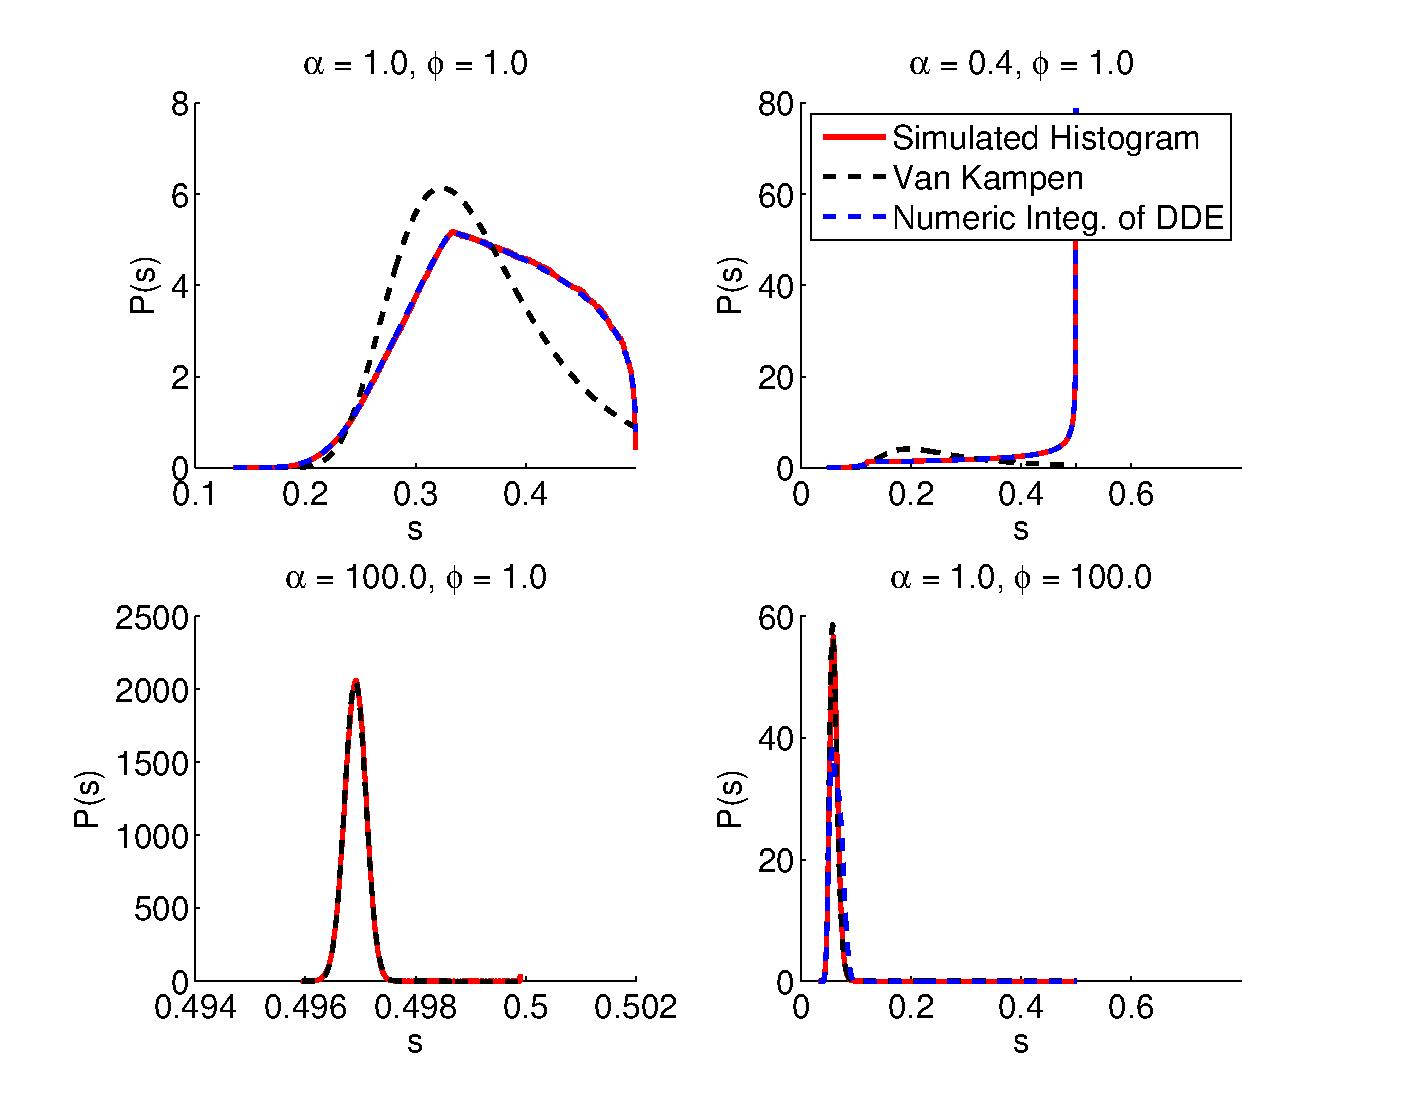
\includegraphics[width=\columnwidth]{figures/figure_3_1.eps}
\caption[Comparison of different solution approaches for the stationary distribution of variances.]{The two approaches to solving for the equilibrium distribution described, shown across a range of parameter values.}
\end{figure}
One particularly interesting characteristic of \fref{eq:dist_1d_exact} is its exponent. The sign of the exponent in \fref{eq:dist_1d_exact} depends on the specific value of $\hat{\lambda}$ 
and $2\gamma$. If $\hat{\lambda} > 2\gamma$, the exponent will be larger than 0, leading the distribution to tend to $0$ as $s$ tends to $s_0$. If, however, 
$\hat{\lambda} < 2\gamma$, the exponent will be negative, leading the distribution to diverge around $s_0$. Notice that $s_0$ is the worst possible performance our encoder can 
achieve, as it is the stationary variance of the unobserved process. This means that whenever the firing rate of the population is below a certain value, the probability distribution of our MSE will 
be dominated by its worst possible value. These results are illustrated in \fref{fig:comparison_histograms}. This is very interesting, as it relates two different time scales, 
one ($1/2\gamma$) describing how long information about the observed process stays relevant, the other ($1/\hat{\lambda}$) describing the average time between observations. It is 
intuitive to say that if the interval between spikes is much larger than the correlation time of
the process, one would expect estimation of the system's state to be bad. But here I have provided a simple analytic argument showing that, for a simple system
whenever the average inter spike interval is longer than the correlation time of the observed process, the mode of the distribution of errors will be the worst possible 
error for the estimator.
\par
Although the obtained distribution is always valid in the interval $S_0$, it can be shown to hold in the limit of low firing rates as well. This 
can be extended numerically to higher dimensions. Assuming the population firing rate $\hat{\lambda} \ll 2\gamma$, one will find that the expected interspike interval is much longer than the 
characteristic time of the variance's dynamics. It is then safe to assume, that whenever a spike is fired, the variance is very close to the stationary variance of the unobserved process 
$\Sigma_0 = \eta/2\gamma$. The 
evolution of it after the spike time $t_s$ will then be given by
\[
\Sigma(t) = e^{-2\gamma(t-t_s)} \Sigma' + \Sigma_0 \left(1-e^{-2\gamma (t-t_s)}\right),
\]
where $\Sigma' = j(\Sigma_0)$.
Solving for the time, one obtains
\[
\tau(\Sigma) \equiv (t-t_s) = -\frac{1}{2\gamma} \log\left(\frac{\Sigma_0-\Sigma}{\Sigma_0-\Sigma'}\right).
\]
Clearly, if the spikes are sampled from a Poisson process, then the interspike intervals have an exponential distribution $P(\tau) \propto e^{-\hat{\lambda}\tau}$. A change of 
variables thus leads to the density
\[
P(\Sigma) = P(\tau) \left|\frac{d\tau}{d\Sigma}\right| \propto e^{-\hat{\lambda} \tau + 2\gamma \tau}.
\]
Inserting the definition for $\tau$ one recovers \fref{eq:dist_1d_exact}. This is an approximation for $P(\Sigma)$ throughout the range of $s$ for a particular parameter limit, whereas before
I had derived an exact result for any parameters, but limited to a small range of values of $\Sigma$.\par

\subsection{An Extension to the Multidimensional Case}

I will derive a similar limit for the multidimensional case. First assume $\hat{\lambda}$ is small enough for the covariance $\Sigma$ to have relaxed to the stationary covariance of the unobserved process $\Sigma_0$. After a spike the covariance is then given by $\Sigma' = \left(\Sigma_0^{-1}+\covar^\dagger\right)^{-1}$. The evolution of $\Sigma(t)$ after a spike at $t_s$ is
\[
\Sigma(\tau) = e^{\tau A} \Sigma' e^{\tau A^\top} + \int_0^\tau e^{t A}\eta e^{t A^\top} dt.
\]
It is not possible to proceed as before, since the mapping from the matrix space of $\Sigma$ to the one-dimensional time space can not be explicitly written as above.
One could try to work out the densities for individual entries of the matrix $\Sigma$ but these would 
possibly not be one-to-one. One alternative is to evaluate the marginals of the matrix entries numerically through integration of the dynamics of $\Sigma(\tau)$.
One could thus integrate $\Sigma(t)$ numerically until it has reached the stationary value $\Sigma_0$, and evaluate the derivatives $\dot{\Sigma}$ numerically. This allows one to
look at the marginal probabilities of each entry of $\Sigma$, leading for example to
\[
P(\Sigma_{11}) = \frac{P(\tau(\Sigma_{11}))}{\left|\frac{d \Sigma_{11}}{d\tau}\right|} \propto \frac{e^{-\hat{\lambda} \tau}}{\left|\frac{d \Sigma_{11}}{d\tau}\right|},
\]
where $\tau(\Sigma_{11})$ is simply the time associated to that particular value of $\Sigma_{11}$ in the numerical integration.
If $A$ introduces interactions between the entries of the covariance matrix, however, this result will not prove as powerful. As an example, consider the Matern processes treated in \mycitep{Susemihl2013}, 
where the unobserved covariance evolves as
\begin{eqnarray*}
\frac{d\Sigma_{11}}{dt} = &2 \Sigma_{12},\\
\frac{d\Sigma_{12}}{dt} = \frac{d\Sigma_{21}}{dt} =& \Sigma_{22} -2 \gamma \Sigma_{11} -\gamma^2 \Sigma_{12},\\
\frac{d\Sigma_{22}}{dt} = & \eta -4 \gamma \Sigma_{12} -2\gamma^2\Sigma_{22}.
\end{eqnarray*}
The numerical approach for this Matern process is shown in \fref{fig:matern_histograms}, and again it coincides well with the distribution in the regime of low firing rates. It is important
to note, that because of the higher-order dynamical nature of the covariance, the divergence of $\Sigma_{11}$ around its stationary value no longer dominates the distribution, as
$\frac{d\Sigma_{11}}{dt}|_{\Sigma'} = 0$, leading to a second peak in the distribution around $\Sigma'_{11}$. 
%Furthermore, even in the limit of low firing rates, the effect of
%consecutive spikes can still be seen due to the slower relaxation of the covariance. This is given by the left side of the histogram in \fref{fig:matern_histograms}.

\begin{figure}
\label{fig:matern_histograms}
\includegraphics[width=\columnwidth]{figures/matern_histogram.eps}
\caption[Distribution of variances in the limit of small firing rates.]{The small firing rate limit for the Matern process.}
\end{figure}

\subsection{Van Kampen Approximation}

It is interesting to consider a different limiting behaviour to gain insight into the fluctuations of $\Sigma$. The Van Kampen approximation is a system size expansion, often
employed in the field of statistical physics. It consists of expanding the transition
probabilities around the deterministic solution in powers of the inverse system size and solving the dynamics of the resulting Focker-Planck equation. It is not evident how to choose
a system size for the problem at hand, but below I will show that it makes sense to consider the quantity $\gamma \alpha^2/\eta$ as a system size. It is simple to apply this
to the OU problem by taking the scaled inverse variance $z= \frac{\eta}{\gamma \Sigma}$ instead of the variance.
Note that although the change in the variance when a spike is observed is nonlinear, the change in the inverse variance is linear. This leads to the ODE
\[
\frac{dz}{dt} = -\gamma z \left(2- z\right) \textrm{ and the jump condition } z(t) = z(t^- ) + \frac{\eta}{\gamma \alpha^2}
\]
for all times $t$ when there is a spike observed. Defining the jump size as $\delta =  \frac{\eta}{\gamma \alpha^2}$, the differential Chapman-Kolmogorov equation for $P(z,t)$ is 
given by
\begin{equation}
\label{eq:DCKE_Z}
\frac{\partial P(z,t)}{\partial t} = \frac{\partial \left( \gamma z \left(2- z\right) P(z,t)\right)}{\partial z} + 
\hat{\lambda}\left[ P\left(z+\delta,t\right) - P(z,t)\right].
\end{equation}
The evolution of the average of $z$ is given by
\[
\frac{d \boldsymbol{E}\left[z\right]}{dt} = -\gamma\boldsymbol{E}\left[ z \left(2-z\right)\right]+ \hat{\lambda}\delta,
\]
which gives the mean-field stationary solution of $z^* =1+\sqrt{1+\hat{\lambda} \delta}$. 
This mean-field approach can be refined by expanding the nonlinear terms in \fref{eq:DCKE_Z} around $z^*$ up to first order, which will yield a linear Focker-Planck equation, which 
can be readily solved. The stationary solution to the Focker-Planck equation is a Gaussian distribution
\[
P_{eq}(z) = \mathcal{N}\left(\left(1+\sqrt{1+\hat{\lambda}\delta}\right), 
\frac{ \hat{\lambda}\delta^2 }{4\gamma \sqrt{1+\frac{\hat{\lambda}\delta}{\gamma} }}\right).
\]
With this solution in hand, it is easy to find the distribution of $\Sigma$ by a change of variables.
This approach is shown in \fref{fig:comparison_histograms} along with the numerical solution of the delayed-differential equation and the numerical simulations. 
Note that, again, \fref{eq:DCKE_Z} is still exact, and one can look at it to determine when the approximation is appropriate. I have Taylor expanded 
$P(z+\delta)$ keeping terms up to first order, and this will yield good approximations whenever $\frac{\eta}{\gamma\alpha^2}$ is small, that is, whenever the tuning width
is large compared to the stationary variance of the unobserved process. Furthermore, the nonlinear term $\gamma z (2-z)$ was also linearised around the mean-field stationary
value, which will only be a good approximation when $z$ has a small probability of wandering far from $z^*$. 
\par

In this case, $\frac{\gamma \alpha^2}{\eta}$ provides a system-size-like quantity for this system, giving us the order of magnitude of the fluctuations of the system. This can be understood
by noting that the change in $\Sigma$ after a jump is given by
$\Delta\Sigma = \frac{\Sigma^2}{\Sigma+\alpha^2}$. The jump can be treated as Gaussian noise if it is very small compared to the value of $\Sigma$, i.e.
\[
\frac{\Delta\Sigma}{\Sigma} = \frac{\Sigma^2}{\Sigma(\Sigma+\alpha^2)} = \frac{\Sigma}{\alpha^2} \frac{1}{1+\frac{\Sigma}{\alpha^2}},
\]
so the size of jumps relative to $\Sigma$ are of the order of $\Sigma/\alpha^2$ and can be safely treated as Gaussian noise if $\alpha^2$ is much larger than the typical value of 
$\Sigma$. $\Sigma$ is at most of the order of $\eta/2\gamma$ so the limit derived above makes sense. If $\gamma\alpha^2/\eta$ is very large, the fluctuations in $\Sigma$ should be 
small, rendering the Van Kampen approximation precise. This is seen to be the case in the lower left panel of
\fref{fig:comparison_histograms}, where the distribution of $\Sigma$ is narrow and the system size is large ($\gamma\alpha^2/\eta = 10000$), leading to a good agreement of the simulations with the 
Van Kampen approximation. In the lower right panel, the Van Kampen also fairs very well, but there the system size is 1. In the derivation above, however, I have used $\eta/\gamma$ as an upper
bound on values of $\Sigma$. As can be glanced from the histogram in the lower right of \fref{fig:comparison_histograms}, the typical value of $\Sigma$ is around $0.05$, due to the high firing rate.
So the actual system size as argued above would be of $\approx 50$, making the Van Kampen approximation justified.

\subsection{Prediction Error}
%Note that it is straightforward to derive 
What if I wanted to predict the value of the stimulus $X$ at a future time, for which I have no spike train information? In the absence of spikes the optimal MMSE estimator is given by 
the evolution of the mean and covariance with $dN^m(t) = 0$, and one would have the predictive probability
$P(X({t+\delta})|\{N^m_{0:t}\})$, with $\delta>0$. Here I am assuming the spikes are only observed up to time $t$, and I am trying to infer $X$ at some future time $t+\delta$.
The mean squared error or prediction error committed when estimating future values of $X$ in that way is given by
\begin{equation}
\boldsymbol{PE}_\delta(t) = \boldsymbol{E}_{X,\{N^m_{0:t}\}}\left[\left(X(t+\delta)-\mu(t+\delta;\{N^m_{0:t}\})\right)\left(X(t+\delta)-\mu(t+\delta;\{N^m_{0:t}\})\right)^\top\right].
\label{eq:C_delta}
\end{equation}
This gives us the matrix $\boldsymbol{MSE}$ when $\delta= 0$. For $\delta>0$ it gives the prediction error matrix.
Given a value of $X(t)$ and a realisation of the Wiener process $W(s)$ for $t\leq s \leq t+\delta$, one has
\[
X(t+\delta) = \int_0^{\delta} e^{-s A} \,H^{1/2} d W(s) + e^{-\delta A}\,X(t).
\]
Clearly, conditioning on $X(t)$ the above average is only over the Wiener process between $t$ and $t+\delta$. The estimator $\mu(t+\delta;\{N^m_{[0,t]}\})$ is also given by $\mu(t+\delta;\{N^m_{[0,t]}\}) = e^{-\delta A} \mu(t;\{N^m_{[0,t]}\})$ in the absence of spikes. The prediction error matrix will then be given by

\begin{eqnarray}
\boldsymbol{PE}_\delta(t)  =& \boldsymbol{E}_{W,\{N^m(0:t)\}}&\left[( \int_0^{\delta} e^{-(\delta-s)A} H d W(t+s) + e^{-\delta A}X(t)-e^{-\delta A}\mu(t))\times\right.\nonumber
\\
&&\left. (\int_0^{\delta} e^{-(\delta-u)A} H d W(t+u) + e^{-\delta A}X(t)-e^{-\delta A}\mu(t))^\top \right].\nonumber
\end{eqnarray}

Since $ e^{-(\delta-u)A} H$ is non-anticipating and does not depend on $X(t)$ or $N^m(t)$, one has that (see \mycitep{Gardiner2004})
$$
\boldsymbol{E}_{W}\left[\int_0^{\delta} e^{-(\delta-u)A} Hd W(t+u) \int_0^{\delta} e^{-(\delta-s)A} H dW(t+s))^\top \right] = \int_0^{\delta} e^{-(\delta-u)A}H^2 e^{-(t+\delta-u)A^\top} d u
$$
and therefore, changing variables,
\begin{equation}
\boldsymbol{PE}_\delta(t)= e^{-\delta A} \epsilon(t) e^{-\delta A^\top} + \int_{0}^\delta e^{-s A} H e^{-s A^\top}d s.
\label{eq:pred_error}
\end{equation}
This equation also describes the evolution of the variance of a linear stochastic processes,\footnote{See \citep[p.106]{Gardiner2004} for an example. This derivation is closely related to 
the derivation of the stationary variance for the OU process therein.} and it shows us that the prediction error is a simple function of the filtering error. This is also a consequence of the 
Markov nature of the posterior probability. Taking a non-Markov prior process would result in a posterior probability whose parameters could not be described by a finite set of ordinary 
differential equations.\par
\Fref{fig:prediction}  shows a comparison between the theoretical result in \fref{eq:pred_error} and simulation results for the prediction error. One can see that the prediction error is very well described by the derived equation.
\begin{figure}
\label{fig:prediction}
\includegraphics[width=.9\columnwidth]{figures/figure_3_3.eps}
\caption[Prediction Error.]{The evolution of the average prediction error $\mathcal{P}(\delta)$ is completely determined by the filtering error $\mathcal{P}(0)$. The blue line shows the prediction error obtained from the optimal filter in simulations, whereas the green line shows the evolution of the prediction error according to \fref{eq:pred_error} with the initial condition given by the average filtering error obtained in the simulations. The small discrepance between both curves is due to finite sample size effects.}
\end{figure}

\section{A Functional Approach to the MMSE}

\label{sec:kernels}

In \fref{sec:gp_filtering}, I have introduced Gaussian Process regression as a method of filtering general Gaussian Processes. So far, I have only considered stochastic processes
which are Markovian or can be rendered Markovian by an embedding into a higher-dimensional stochastic process.\footnote{See \fref{sec:stochastic_proc}} It is easy to adapt the
treatment given in \fref{sec:gp_filtering} to the case of Poisson processes. Say I am given a Gaussian process with zero mean and covariance function $K(s,v)$ and spike trains
from a dense population of Gauss-Poisson neurons. Assuming up to time $t$ there have been $M$ spikes, at times $\{t_i\}$ fired 
by neurons $\{n_i\}$ and the tuning centres of the spiking neurons are given by $\boldsymbol{\theta} = (\theta_{n_1}, \ldots, \theta_{n_M})^\top$, the posterior mean and covariance are
\begin{equation}
\mu(t) = k(t,\{t_i\})^\top (G + \alpha^2 \boldsymbol{I})^{-1} \boldsymbol{\theta},
\end{equation}
and
\begin{equation}
\Xi(t,t) =  K(t,t) - k(t,\{t_i\})^\top (G+\alpha^2\boldsymbol{I})^{-1} k(t,\{t_j\})^\top.
\end{equation}
Here $G_{i,j} = K(t_i,t_j)$ and $\alpha^2$ is the width of the tuning functions. The covariance of the posterior distribution at two
points is given by
\[
\Xi(s,t) = k(s,t) - \sum_{i,j} k(s,t_i) C_{ij} k(t_j,t).
\]
I will call the quantity $\Xi(s,t)$ the posterior kernel, as it again defines a GP. According to the formalism derived so far the MMSE for a filtering 
problem is simply the expected value of the posterior kernel $\Xi(t)$ averaged over the distribution of all possible past observations. Like I have done for the 
MMSE, I can look into the dynamics of the posterior kernel $\Xi(s,t)$. Defining $f_t(u,v) = \Xi(t+u,t+v)$, one has
\[
\frac{\partial f_t(u,v)}{\partial t} = \left( \frac{\partial }{\partial u}+ \frac{\partial }{\partial v}\right) f_t(u,v).
\]
It is a simple exercise in matrix inversion lemmas to show that, if a observation is obtained at time $t$ the posterior kernel will change as
\[
f_t(u,v) = f_{t^-}(u,v) - \frac{f_{t^-}(u,0)f_{t^-}(0,v)}{\alpha^2+ f_{t^-}(0,0)}.
\]
Taking the average over all possible observation paths one obtain the evolution of the average posterior kernel
\[
\frac{\partial \boldsymbol{E}\left[f_t(u,v)\right]}{\partial t} = \left( \frac{\partial }{\partial u}+ \frac{\partial }{\partial v}\right) \boldsymbol{E}\left[f_t(u,v)\right] - \hat{\lambda}\boldsymbol{E} \left[\frac{f_{t}(u,0)f_{t}(0,v)}{\alpha^2+ f_{t}(0,0)}\right].
\]
Again, I am most interested in the stationary case, so setting the derivative to zero one obtains
\begin{equation}
\label{eq:differential_kernel}
\left( \frac{\partial }{\partial u}+ \frac{\partial }{\partial v}\right) \boldsymbol{E}\left[f(u,v)\right] = \hat{\lambda} \boldsymbol{E}\left[\frac{f(u,0)f(0,v)}{\alpha^2+ f(0,0)}\right].
\end{equation}
Using the mean-field approximation leads to
\begin{equation}
\label{eq:kernel_mf}
\left( \frac{\partial }{\partial u}+ \frac{\partial }{\partial v}\right) \boldsymbol{E}\left[f(u,v)\right] = \hat{\lambda} \frac{ \boldsymbol{E}\left[f(u,0)\right]  \boldsymbol{E}\left[f(0,v)\right] }{\alpha^2+  \boldsymbol{E}\left[f(0,0)\right] }.
\end{equation}
This is solved by the integral equation
\begin{equation}
\label{eq:integral_kernel}
\boldsymbol{E}\left[f(u,v)\right] = k(u,v) - \frac{\hat{\lambda}}{\alpha^2+ \boldsymbol{E}\left[f(0,0)\right]} \int_0^\infty \boldsymbol{E}\left[f(s+u,0)\right]\boldsymbol{E}\left[f(0,s+v)\right] ds,
\end{equation}
as long as the kernel $k(u,v)$ is stationary, which implies $\partial_u k(u,v) = - \partial_v k(u,v)$.\footnote{A stationary kernel is such that 
$k(t,v) = k(\|t-v\|)$. If $t > v$ and $t> v+d$, then $k(t,v+d) = k(t-d,v)$. Differentiating with respect to $d$ we obtain the desired result.}\par

\Fref{eq:integral_kernel} allows one to approximate the shape of the posterior kernel directly from the prior kernel, without having to resort to the Markovian structure of
the process as we had done before. This is very convenient as it allows one to treat non-Markovian GP's such as the one defined by the squared exponential or Radial
Basis Function kernel.\footnote{The SE or RBF kernel is given by $k(t,v) = c \exp(-|t-v|^2/L^2)$.} This relies on the Mean-field approximation, but it is
still a very pleasing result, as it additionally allows one to estimate the shape of the entire posterior kernel, not only of the one-time variance. If one is only interested
in the filtering error however, it suffices to take the function $g(u) = \boldsymbol{E}\left[f(u,0)\right]$, where the filtering error is then given by $g(0)$. For that the equation simplifies to
\begin{equation}
\label{eq:integral_one_point}
g(u) = k(u,0)  - \frac{\hat{\lambda}}{\alpha^2+ g(0)} \int_0^\infty g(s+u)g(s) ds
\end{equation}
One way to solve \fref{eq:integral_one_point} is to simply discretise the real line over some interval $[0,D]$ and iterate \fref{eq:integral_one_point} numerically. I will discuss this approach shortly in \fref{app:kernel_integral}. This is shown in \fref{fig:integral_kernel} for the OU kernel $k_{OU}(s,t) = \exp(-|s-t|/k)$, for the Matern kernel $k_{mat}(s,t) = (1+\sqrt{3}|t-s|/k) \exp(-\sqrt{3}|t-s|/k)$ and the 
RBF kernel $k_{dbf} = \exp(-|t-s|^2/2k^2)$. As one moves towards smoother processes, the variance of the posterior kernel decreases, and the effect of the observations becomes more pronounced.

\begin{figure}
\label{fig:integral_kernel}
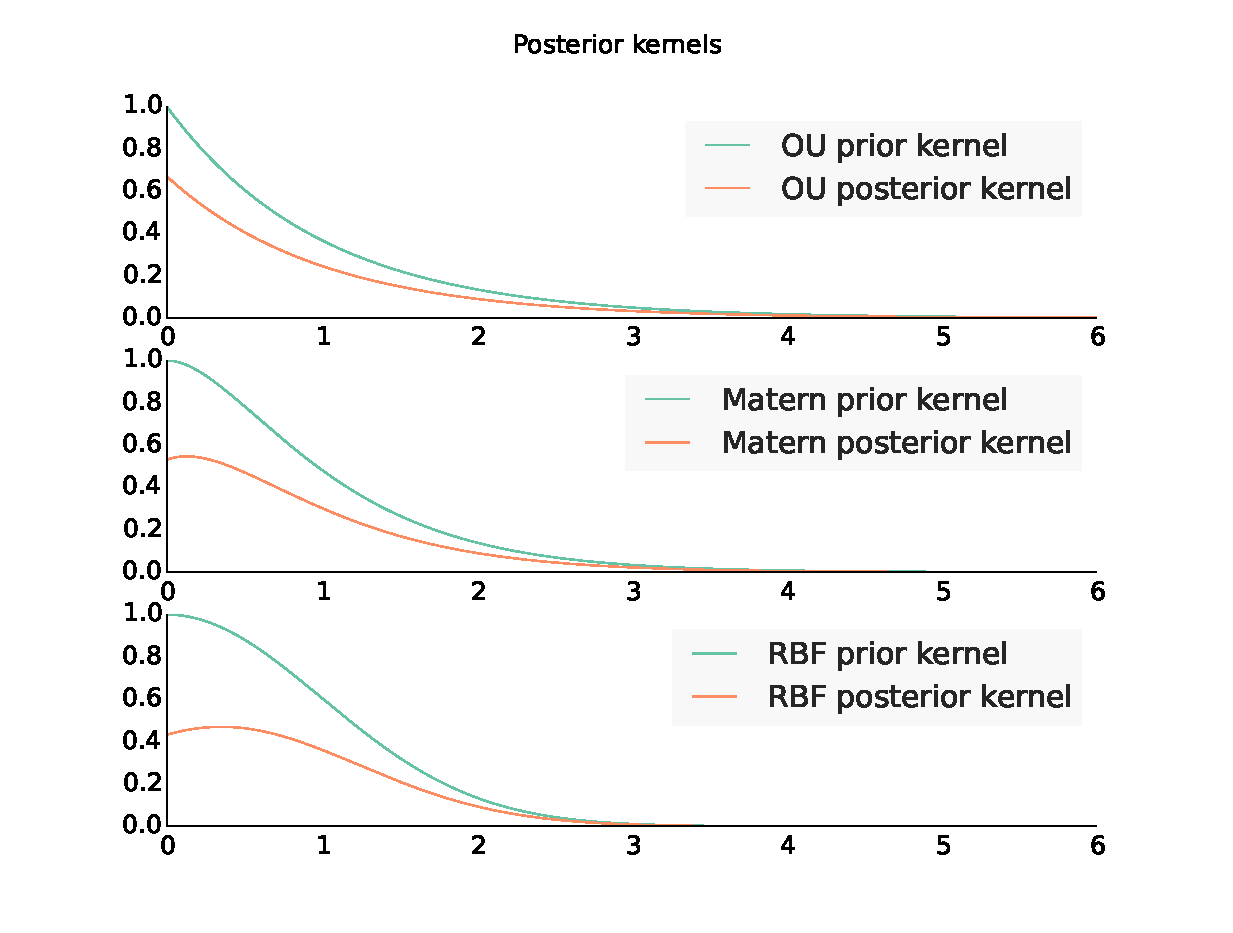
\includegraphics[width=\columnwidth]{figures/figure_3_4.eps}
\caption[Posterior kernels for general Gaussian processes]{The prior and posterior kernels for the filtering problem for three classes of GP's.}
\end{figure}

This can be used to study the MMSE of more complex Gaussian processes. The RBF kernel and the associated Gaussian process have been the subject of great
interest, specially in the Machine Learning community, as the squared exponential form of it often allows one to simplify a number of expressions in Gaussian
averages. Marc Deisenroth, for example, proposed to use the Gaussian form of the RBF kernel to average over uncertainty in the input $t$ of the process 
as
well as in the observation $Y$.\mycite{deisenroth2009} However, though it has proven very useful in ML, the RBF kernel is often criticised for being too smooth.\mycite{Rasmussen2005} 
A function $f(s)$ drawn from a GP with an RBF kernel is $\mathcal{C}^\infty$, leaving little room for randomness in its proper sense. On the other hand, \mycitet{Huys2007} have argued
that experimental trajectories of freely moving animals show an autocorrelation that is compatible with the RBF kernel. Though it might be a too strong prior to impose on natural 
stimuli, the RBF kernel might still be useful to model animal behaviour, with its longer time dependence.

\section{Alternative Performance Measures for Estimation}

I have chosen to focus on the mean-squared error of an estimation problem as a measure of efficiency of a neural population code. This is by no means the
only alternative there is. Many studies in computational neuroscience have focused on the Fisher information,\mycite{Ganguli2011,Zhang1999a,Brunel1998} and information-theoretical 
quantities such as the entropy or the mutual information of a code.\mycite{Schneidman2003,Tkacik2010,,Brunel1997} I will review the motivation and discuss the application of these tools in 
the present setting if merited.

\subsection{Fisher Information}
\label{sec:fisher_info}

The Fisher information gives an alternative measure to the amount of information carried by an observation $Y$ about an unobserved parameter or variable $x$.
The Fisher information $\mathcal{I}(x;Y)$ of $Y$ about $x$ is given by
\begin{equation}
\mathcal{J}(x;Y) \equiv \int P(Y|x) \left(\frac{\partial \log\left(P(Y|x)\right)}{\partial x}\right)^2 dY.
\end{equation}
Intuitively, the Fisher information tells one how sensitive the likelihood of an observation is to a change in the unobserved variable $x$ at that particular value. So,
a code that gives a high Fisher information on average will be very sensitive to changes in $x$, allowing for good estimation of $x$ from $Y$.
The relationship between estimation and the Fisher information can be made rigorous through the Cram\'{e}r-Rao bound. If one has an estimator
$\hat{x}(Y)$ of $x$ based on observations of $Y$, the Cram\'{e}r-Rao bound states that the variance of that estimator is bounded by
\begin{equation}
\label{eq:crb}
\boldsymbol{E}_{Y|x} \left[\left(\hat{x}(Y) - x\right)^2\right]  \ge \frac{\left(1+\frac{\partial b(x)}{\partial x}\right)^2}{\mathcal{J}(x;Y)},
\end{equation}
where $b(x) = \boldsymbol{E}_{Y|x}[\hat{x}(Y)] - x$ is the bias of the estimator. If $\hat{x}(Y)$ is unbiased this simplifies to
\[
\boldsymbol{E}_{Y|x} \left[(\hat{x}(Y) -x)^2\right]  \ge \frac{1}{\mathcal{J}(x;Y)}.
\]
In the multivariate case this becomes a restriction on the positive-definiteness of the MSE matrix, more precisely, for the unbiased case, one has that for any
$v$ it holds that 
\[
v^\top \boldsymbol{E}_{Y|x} \left[(\hat{x}(Y) -x)(\hat{x}(Y) -x)^\top\right] v \ge v^\top \mathcal{J}(x;Y)^{-1} v,
\]
which means that the matrix $\boldsymbol{E}_{Y|x} \left[(\hat{x}(Y) -x)(\hat{x}(Y) -x)^\top\right]-\mathcal{J}(x;Y)^{-1}$ is positive semidefinite.\par

The Cram\'{e}r-Rao bound can also be extended to a Bayesian setting, where one is no longer estimating a fixed parameter but a random variable. Considering $X$
a random variable with distribution $P(X)$, one obtains the Bayesian Cram\'{e}r-Rao Bound (BCRB),
\[
\boldsymbol{E}_{X,Y} \left[\left(\hat{X}(Y) - X\right)^2\right]  \ge \frac{1}{\boldsymbol{E}_X\left[\mathcal{J}(X;Y)\right] + \mathcal{I}(X)},
\]
where
\[
\mathcal{I}(X) = \int dX P(X) \left(\frac{\partial \log P(X)}{\partial X}\right)^2.
\]
Unlike the Cram\'{e}r-Rao Bound given in \fref{eq:crb}, the BCRB gives a bound on the performance of a given code in an environment regardless of the 
system's state.\par

The Fisher information is particularly popular in the neuroscience community partly because it has a convenient form for rate-based models. Suppose one has a Poisson neuron
with some tuning function $f(X)$. The probability of a spike count $r$ in a time interval of duration $T$ is given by
\[
P(r|X) = \frac{e^{-T f(X)T}(T f(X))^r}{r!}, \quad \log(P(r|X)) = r \log (T f(X)) - T f(X) - \log r!.
\]
This leads to the Fisher information
\[
\mathcal{J}_{Poiss} (X;Y) = T \frac{f'(X)^2}{f(X)} = \frac{(T f'(X))^2}{T f(X)},
\]
which is a function of $T f(X)$, the expected number of spikes for the experiment. In \fref{fig:fisher_info} I have shown the Fisher
information for a Gaussian tuning function as a function of $X$.

\begin{figure}
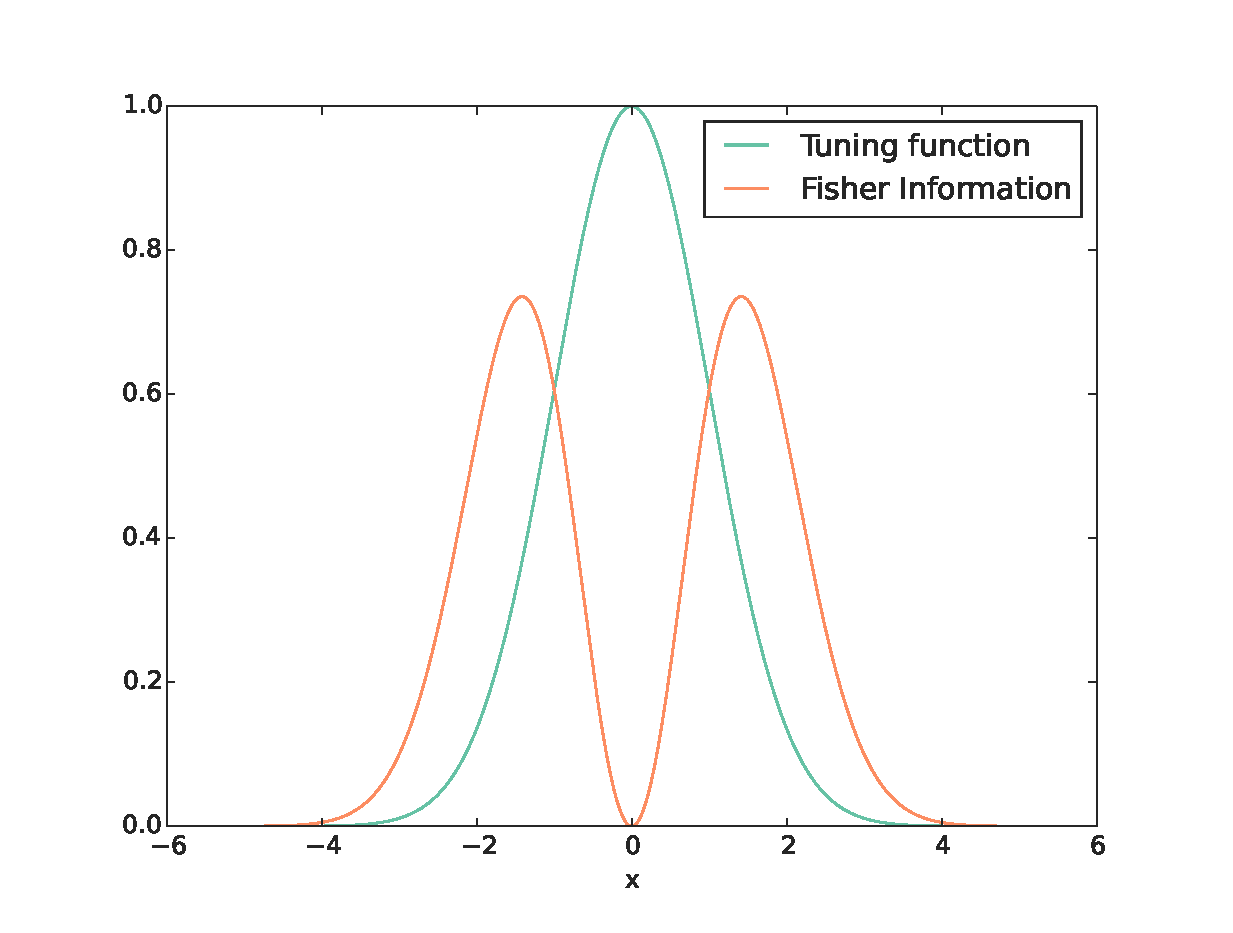
\includegraphics[width=\columnwidth]{figures/figure_3_5.eps}
\caption[Fisher Information for a Gauss-Poisson neuron.]{The Fisher information of a Gaussian-shaped tuning function. Note how the information is highest around the slopes of the tuning function. This approach
puts a higher prize on discriminability, so the highest information is achieved when the slope of the tuning function is highest.}
\label{fig:fisher_info}
\end{figure}

\par
One can see why this is of interest for
computational neuroscientists, as rate-based models are the bread and butter of spike train analysis. A number of experiments sought to use the Fisher information
as a measure of performance for coding strategies, such as \mycitep{Zhang1999a,Brunel1998} for example. More recently, this line of reasoning has been criticised
by a number of findings. Matthias Bethge, for example, argued that the Cram\'{e}r-Rao bound is loose in general and only provides a tight bound on the MMSE of a
neural population code in the limit of very long times and many spikes, rendering it of limited usability.\mycite{Bethge2002} For the dynamic setting I am considering,
where the dynamic nature of the stimulus is central, Fisher information seems to be of little use. \mycitep{Yaeli2010} and \mycitep{Berens2011} have compared the MMSE with
the Cr\'{a}mer-Rao bound extensively, coming repeatedly to the conclusion that the Cr\'{a}mer-Rao bound leads to troubling results, such as the optimal
code not depending on the decoding time available. I will therefore not spend any further time investigating the Fisher information in this thesis.

\subsection{Mutual Information}
\label{sec:mutual_info}

The canonical tool to quantify the level of dependence between two variables in information theory is the mutual information. Though the correlation is often 
preferred, the mutual information provides the guarantee that it is zero if and only if the random variables are statistically independent, providing a way of robustly quantifying the level 
of dependence between two variables. The mutual information was defined in \fref{chap:intro} as
\[
I(X;Y) = \int dX dY P(X,Y) \log \left(\frac{P(X,Y)}{P(X)P(Y)} \right),
\]
which can be readily cast into
\[
I(X;Y) = \int dX dY P(Y) P(X|Y) \log \left(\frac{P(X|Y)}{P(X)} \right) = \boldsymbol{E}_Y \left[H(X) - H(X|Y)\right],
\]
which gives the average reduction of entropy in $X$ upon observing a random value of $Y$.  One advantage of the mutual information is that it does not make
any reference to an estimator or a reconstruction procedure, giving us a principled quantification of the information obtained about one variable from an observation
of the other. The main disadvantage of the mutual information is that it is much harder to compute than other quantities, as one is required to estimate the whole
probability distribution of $X$ and $Y$ to do so.\par

Another important issue one should note, is that the interpretation of the mutual information as an reduction of the entropy is more problematic in the continuous case. As I had noted 
before, the differential entropy can given negative values, making the last step of the equation above a bit delicate. Furthermore, the mutual information between two continuous 
random variables is only defined if their densities are absolutely continuous with respect to each other. In the sense of probability theory, this means that the mutual information is only
defined if, whenever $P(X,Y) > 0$ then $P(X)P(Y) > 0$. The probability densities I am considering here are mostly Gaussian, and therefore positive through their whole domain, so
this will not be an issue in the present case.\par

More recently, there have also been a number of results relating the mutual information to the MMSE of estimators. One of the most surprising results is probably is that for an additive
Gaussian channel, where one is trying to estimate the value of a random variable $X$ from an observation of $Y = k^{1/2} X + N$, the following relationship holds
\[
\frac{\partial I(X;Y)}{\partial k} = \frac{1}{2} MMSE(\hat{X}(Y)).
\]
This holds regardless of the distribution of the random variable $X$.
This is one of the so-called I-MMSE relations, which have been a very popular area of study in the field of information theory recently.\mycite{guo2005,wu2010,merhav2011}

For the dense Gauss-Poisson populations under consideration one can evaluate the mutual information readily. Assume that at time 0, knowledge of the
system's state $X$ is given by some normal distribution $P_0(X)$. One can then easily evaluate the mutual information of the system's
state at time $t$, $X(t)$ and the spike train up to time $t$, $N_{0:t}$. To that end, one needs only to note that the marginal $P(X(t))$ is given by a Gaussian with
moments evolving according to \fref{eq:free_ou_moments}, which I will denote as $\mu^0(t)$ and $\Sigma^0(t)$. The posterior distribution is given simply
by the solution of the filtering equations for the problem. The distributions are given by
\[
P(X(t)) = \mathcal{N}(\mu^0(t),\Sigma^0(t)), \textrm{ and } P(X(t) | N_{0:t}) = \mathcal{N}(\mu(t; N_{0:t}), \Sigma(t; N_{0:t})),
\]
and therefore
\[
I(X(t);N_{N_{0:t}}) = \log |\Sigma^0(t)| - \boldsymbol{E}_{N_{0:t}}\left[\log |\Sigma(t; N_{0:t})|\right].
\]
Here again, one is faced with an average over $P(\Sigma,t)$, this time of the logarithm of the determinant of $\Sigma(t)$. In the mean-field approximation, this will give simply the
logarithm of the determinant of the matrix $\epsilon(t)$. I will show in \fref{chap:optimal} that the mutual information leads to the same optimal codes as the MMSE for the OU process.



\chapter{Optimal Control with Point Process Observations}

\label{chap:control}

\newthought{Clearly the nervous system is not solely interested in estimating the state of the world.} Furthermore, if that estimate is not useful for making decisions and taking actions in a dynamic environment, there is little use for it. In the previous chapter I have discussed findings for spiking codes in an estimation context. In this chapter I will extend this approach to the framework of stochastic optimal control, and discuss how to reframe the findings in this context.\par

\section{Estimation and the Separation Principle}

In the previous two chapters, I have considered the filtering problem based on spike trains. More specifically, given a signal, we were looking for the optimal set of parameters for a population of neurons $\boldsymbol{\theta}^*$ that minimize the MSE of the filtering problem. If we are interested in controlling a system, say a limb performing a movement, the picture changes somewhat. It is very usual for control problem to use the separation principle\cite{Bar-Shalom1974} to develop approximate solutions to control problem. The separation principle considers a control problem with incomplete information as a sequence of two independent problems. The first one is to estimate the state from the observed processes. The second one is to solve some complete information control problem associated to the incomplete information problem we are considering. Then the separation approach to control would be to apply the complete information optimal control on the mean estimate of our state. This approach, and a stronger version of it, the Certainty Equivalence Principle, hold in a number of situations, making the separation principle one of the most important tools in control theory. However, even if one can separate both steps in the control setting, one can not expect optimal encoders for the filtering problem to yield optimal encoders for the control problem.\par
I will in this chapter consider control problems where the system is observed through noisy spike trains. The optimal encoding strategies will in this case be the ones that minimize the control cost, not the MSE. Though these quantities turn out to be related when the state cost is quadratic, I will show a couple of simple examples where the MSE-optimal encoder is drastically different from the control-optimal encoder. Although these results are quite intuitive, as one expects sensory systems to devote more energy to coding for aspects of the environment which are important for their well-being or survival, this approach has been completely overlooked in the optimal population coding literature.

\section{Optimal Control}
The field of control theory is concerned with the steering and controlling of systems, always with the minimization of a cost (or maximization of a reward) in mind. Speaking mathematically, given a system $X$, with dynamics given by
$$
\dot{X}_t = f(X_t,u_t),
$$
we would like to select the control variables $u_t$ in such a way as to minimize an integrated cost function over time
$$
C(X,u,t) = \int_{t}^T c(X_s,u_s,s) ds.
$$
The solution of a control problem is frequently given as a policy $\pi$, a function of the state space to the space of controls. One would have\marginnote{The minimum of the future cost over the space of controls is called the value function $V(X,t)$.}
$$
\min_u C(X,u,t) = C(X,\pi(X),t) \equiv V(X,t).
$$
Clearly this formulation is too broad to allow for any useful development. One general remark to be made, though, is one first made by Richard Bellman. Bellman\cite{Bellman1952} proposed an optimality principle\marginnote{Bellman's principle of optimality}, which stated that if a given policy is an optimal solution to a control problem, than the policy resulting after a number of steps of that policy must still be optimal for the remaining control problem as well. This can be formulated as a mathematical equation, the so-called Bellman equation or dynamic programming equation, which states that the minimal future cost in state $X_t$ at time $t$ is given by the minimum over $u_t$ of the instantaneous cost plus the minimal future cost at the resulting future state $X_{t+dt}$. Mathematically, we have
$$
V(X_t,t) = \min_{u_t} \left[ c(X_t,u_t,t) dt +V(X_{t+dt},t+dt)\right].
$$
Note that in general, $X_{t+dt}$ will depend on $u_t$, making the solution of the Bellman equation difficult.\par
In continuous time, one can assume differentiability of the value function $V$ in both its arguments to obtain the Hamilton-Jacobi-Bellman equation\marginnote{We will abbreviate the Hamilton-Jacobi-Bellman equation as HJB equation.}. We have
$$
V(X_t,t) = \min_{u_t} \left[c(X_t,u_t,t) dt + V(X,t) + \frac{\partial V}{\partial t} dt + \frac{\partial V}{\partial X} dX_t \right],
$$
which gives us then
$$
-\frac{\partial V}{\partial t} = \min_{u_t} \left[c(X_t,u_t,t) + \frac{\partial V}{\partial X} f(X_t,u_t) \right].
$$
This is often more convenient to solve, as it sometimes allows for explicit minimization over the control.

\subsection{Stochastic Optimal Control}

The world is a noisy place, and if we want to control real-world systems, we must be able to account for noise in the systems as well. One simple way to include noise is to generalize the system dynamics to a stochastic differential equation. We would then have
$$
dX_t = f(X_t,u_t) dt + \sigma dW_t,
$$
where $dW_t$ is a zero mean, unit variance Wiener process.
The HJB equation can then be calculated through It\=o's lemma, yielding
$$
-\frac{\partial V}{\partial t} = \min_{u_t} \left[c(X_t,u_t,t) + \frac{\partial V}{\partial X} f(X_t,u_t) + \sigma \frac{\partial^2 V}{\partial X^2} \right].
$$
Note that we could also have a Poisson process as a noise source. If we take, for example, a Poisson counting process $N_t$, with time-dependent rate $\lambda(t)$, and take the system dynamics to be
$$
dX_t = f(X_t,u_t) dt + \sigma dW_t + h(X,t) dN_t,
$$
we would have then, similarly
$$
-\frac{\partial V}{\partial t} = \min_{u_t} \left[c(X,u_t,t) + \frac{\partial V}{\partial X} f(X_t,u_t) + \frac{\sigma}{2} \frac{\partial^2 V}{\partial X^2} + \lambda(t) \left(V(X+h(X,t),t)-V(X,t)\right)\right],
$$
now including the terms regarding the jump process.\cite{Theodorou2012,Sennewald2006} I will use this formalism to treat a simple control problem where the observations are taken from a spike train of Gaussian-tuned Poisson neurons.

\subsection{Linear-Quadratic-Gaussian Control}

The simplest stochastic control problem, is the case of a linear stochastic differential equation with linear steering and quadratic costs both in the control as in the state variables. This would mean that the evolution of the state is given by the SDE
\begin{equation}
\label{eq:ctl_diff_dyn}
dX_t = \left(a X_t + b u_t\right) dt + \sigma dW_t,
\end{equation}
where $W_t$ is a Wiener process. Taking a path cost given by $c(X,u,t) = \frac{1}{2} r(t) u^2 + \frac{1}{2} q(t) X^2$, and a final cost given by $h(X) = \frac{1}{2} Q_T X^2$, we can solve the problem explicitly, using the HJB equation. The HJB equation will be given by
$$
-\frac{\partial V}{\partial t} = \min_{u_t} \left[\frac{1}{2} r(t) u_t^2 + \frac{1}{2} q(t) X_t^2 + \frac{\partial V}{\partial X} \left(aX_t  + bu_t\right) + \frac{1}{2}\sigma^2 \frac{\partial^2 V}{\partial X^2} \right].
$$
We can minimize the right hand side explicitly and eliminate $u_t$ from the equation. We obtain that the optimal value of the control is given by
$$
u^*_t = -\frac{b}{r(t)} \frac{\partial V}{\partial X}.
$$
Inserting into the HJB equation once more, we obtain
$$
-\frac{\partial V}{\partial t} = \frac{1}{2} q(t) X^2 +\frac{\partial V}{\partial X} a X - \frac{b^2}{2 r(t)} \left(\frac{\partial V}{\partial X}\right)^2 + \frac{1}{2}\sigma^2 \frac{\partial^2 V}{\partial X^2}.
$$
We note that $V$ can only have a quadratic dependence in $X$, and we therefore assume it is of the form $V(X,t) = S(t) X^2/2 + \alpha(t) X + k(t)$. We then obtain\marginnote{These equations generalize directly to the multidimensional case, see \ref{app:lqg}}
$$
-\dot{S} = \frac{1}{2} q(t) + a S(t) - \frac{b^2}{2 r(t) } S(t)^2,
$$
$$
-\dot{\alpha} = a \alpha(t)-\frac{b^2}{r(t)} S(t)\alpha(t),
$$
$$
-\dot{k} = \sigma^2 S(t)-\frac{b^2}{2 r(t)} \alpha^2(t),
$$
with the terminal conditions $S(T) = Q_T$, $\alpha(T) = 0$ and $k(T)=0$. Note that the $X$ independent term $k(t)$ accounts for the future uncertainty of $X$, decreasing to $0$ over time as we approach the final time $T$. Furthermore, the differential equation for $S(t)$ is a special case of the Riccati equation.\footnote{See \ref{app:lqg} for a full account of the Riccati equation} These results can also be extended to the case of control- and state-dependent diffusion noise, affine dynamics and some other issues. For a more complete review, we refer to the work of Kappen\cite{Kappen2011}.

\section{Partially Observable Processes}

In general, one does not have access to the exact state of the system, and it is useful to consider cases where we are only given noisy observations of the state, as we have considered in the previous chapters. The most commonly considered case of partially observable control problem is a LQG problem observed through a second diffusion process. Suppose we have as above a system $X_t$ evolving according to equation \fref{eq:ctl_diff_dyn}, but instead of observing $X_t$ directly, we observe the process $Y_t$, which I shall call the observation process, which evolves according to
\begin{equation}
\label{eqn:ctl_obs_dyn}
dY_t = c X_t dt + \eta^{1/2} dV_t.
\end{equation}
Given a control trajectory ${u_s, s\in [0,t]}$, the problem of estimating $X_t$ given observations ${Y_s, s \in [0,t]}$, is a simple filtering problem, and is solved exactly by the Kalman-Bucy filter. We will have a Gaussian estimate of $X_t$ with mean $\mu(t)$ and variance $\Sigma(t)$, where $\mu$ and $\Sigma$ evolve according to
\begin{subequations}
\begin{equation}
d\mu = (a \mu + b u)dt + \Sigma(t) c^t \eta^{-1} \left(dY_t - c\mu dt\right),
\label{eq:ctl_kalman_bucy_mean}
\end{equation}
and
\begin{equation}
\label{eq:ctl_kalman_bucy_var}
\frac{d\Sigma}{dt} = a \Sigma + \Sigma a^\top + \sigma^\top \sigma - \Sigma c^\top \eta^{-1} c \Sigma.
\end{equation}
\end{subequations}
Since in this case we do not have perfect information on the process to be controlled, we have to settle for the goal of minimizing the expected cost given our observation. Therefore, we have the cost to be minimized
$$
C(u_{t_0:T};\mu_0,\Sigma_0) = E\left(\int_{t_0}^T c(X_t,u_t,t)dt +h(X_T)\right).
$$
There is no analogous to the HJB equation for the incomplete information case, but we can reformulate the problem as a control problem over the belief states, that is the state of the world as we are led to believe it is distributed given the previous observations\marginnote{The belief state is a description of an system with incomplete information which eschews describing the actual state of the system, instead describing the distribution over states. A general formulation is described in \citep{bertsekas2012}.}. In the case I am discussing, the belief state is the distribution over the state variable, given by the Gaussian distribution $\mathcal{N}(\mu(t),\Sigma(t))$. The dynamics of the belief state is then given by equations \fref{eq:ctl_kalman_bucy_mean} and \fref{eq:ctl_kalman_bucy_var}. Note that when we choose to describe the system in terms of the mean and variance of the posterior distribution, the noise process $dW_t$ does not enter into the analysis anymore, and the observation process $dY_t$ takes the role of the noise process. We need, however, to redefine the cost function $c(X_t,u_t,t)$ to fully specify the problem. We have that
$$
\left<c(X_t,u_t,t)\right>_{\mu(t),\Sigma(t)} = \frac{1}{2} u_t^\top R(t) u_t + \frac{1}{2}\left(\mu(t)^\top Q(t) \mu(t) + tr\left(Q(t)\Sigma(t)\right)\right).
$$
We can now write the HJB equation for this system. We have
$$
V(\mu(t),\Sigma(t),t) = \min_{u_t} E\left[\frac{1}{2} u_t^\top R(t) u_t+\frac{1}{2}\left(\mu(t)^\top Q(t) \mu(t) + tr\left(Q(t)\Sigma(t)\right)\right)+V(\mu(t+dt),\Sigma(t+dt),t+dt)\right],
$$
where the expectation is now with respect to the observation process $Y(t)$.
Taking now the variation of $V$ with infinitesimal time increments via It\=o's lemma and minimizing over $u_t$, we have
$$
dV = \frac{\partial V}{\partial t} dt + \frac{\partial V}{\partial \mu}^\top d\mu + Tr\left[\frac{\partial V}{\partial \Sigma}d\Sigma\right] + Tr\left[(\Sigma c^\top \eta c \Sigma)_{i,j} \frac{\partial^2 V}{\partial \mu^2}\right].
$$
Which leads to the HJB equation
\[
-\pd{V}{t} = \min_{u_t} E\left[\frac{1}{2} u_t^\top R(t) u_t+\frac{1}{2}\left(\mu(t)^\top Q(t) \mu(t) + tr\left(Q(t)\Sigma(t)\right)\right) +\frac{\partial V}{\partial \mu}d\mu^\top + Tr\left[\frac{\partial V}{\partial \Sigma}d\Sigma\right] + Tr\left[(\Sigma c^\top \eta c \Sigma)_{i,j} \frac{\partial^2 V}{\partial \mu^2}\right] \right].
\]
Minimization with respect to $u_t$ leads to $u^*_t = -R(t)^{-1} b^\top \pd{V}{\mu}$. We will then have
\[
-\pd{V}{t} = \mu^\top Q(t)\mu + \pd{V}{\mu}^\top b R(t) b^\top \pd{V}{\mu} + tr\left(Q(t)\Sigma(t)\right)\right) +\frac{\partial V}{\partial \mu}d\mu^\top + Tr\left[\frac{\partial V}{\partial \Sigma}d\Sigma\right] + Tr\left[(\Sigma c^\top \eta c \Sigma)_{i,j} \frac{\partial^2 V}{\partial \mu^2}\right] \right].
\]
\section{Partially Observable Processes with Poisson Observations}

Similarly to the case just discussed, we can consider the case of a stochastic system observed through a population of densely tuned Poisson processes with Gaussian tuning functions. The dynamics of the system would be the same as \fref{eq:ctl_diff_dyn}, but the observation processes would be given by a set of $M$ Poisson processes $N^m$ with rates given by
\begin{equation}
\label{eq:ctl_poisson_rate}
\lambda^m(X_t) = \lambda \exp\left[-\frac{1}{2}(\theta^m-X_t)^\top A^\dagger (\theta^m-X_t)\right].
\end{equation}
As we have shown in \fref{chap:filtering}, the estimation problem is solved by the point-process analog of the Kalman-Bucy filter, first derived by Donald Snyder and used extensively since\cite{Snyder1972,Yaeli2010}. In our case, with Gaussian tuning functions, we would have the filtering equations given by
\begin{subequations}
\begin{equation}
\label{eq:ctl_poisson_mean}
d\mu_t = (a\mu_t + b u_t) dt + \sum_m dN^m_t \Sigma_t \left(\Sigma_t + A\right)^{-1} \left(\theta_m - \mu_t\right) 
\end{equation}
and
\begin{equation}
\label{eq:ctl_poisson_var}
d\Sigma_t =\left(a \Sigma_t + \Sigma_t a^\top + \sigma^\top\sigma\right)dt - dN_t \Sigma_t \left(\Sigma_t + A\right)^{-1} \Sigma_t,
\end{equation}
\end{subequations}

where $dN_t = \sum_m dN^m_t$. We will define 
$$\delta \mu_t \equiv (a\mu_t + b u_t) dt$$ as the continuous part of $d\mu_t$ and 
$$\Delta^m \mu_t \equiv \Sigma_t \left(\Sigma_t + A\right)^{-1} \left(\theta_m - \mu_t\right) $$ as the jump part of $d\mu_t$. Likewise we define
$$\delta\Sigma_t \equiv (a\Sigma_t + \Sigma_t a^\top + \sigma^\top \sigma)dt$$ and $$\Delta\Sigma_t \equiv \Sigma_t \left(\Sigma_t + A\right)^{-1} \Sigma_t.$$\par
These give us the evolution of the optimal Bayesian filter, provided the total rate of all the processes $\lambda (t) = \sum_m \lambda^m(X_t)$, is independent of $X_t$. The posterior distribution over $X_t$ given $\{N^m_s, m\in [1,\ldots,M], s\in[t_0,t]\}$, is then the normal distribution $\mathcal{N}(X_t;\mu_t,\Sigma_t)$. Assuming we are trying to minimize a cost given by the same cost rate $c(X_t,u_t,t)$ as before, we can write out the infinitesimal Bellman equation for this case as well. Since the dynamics of system and observations is Markov, we can use the posterior distribution as a sufficient statistic for our knowledge of the system. We will therefore take our belief state to be the mean and variance of our posterior distribution as before.\footnote{see \citep{bertsekas2012} for a more detailed discussion}
Similarly to the previous sections, we will consider the processes $N^m_t$ as noise to be averaged over in the future. We will then have
$$
V(\mu_t,\Sigma_t,t)= \min_{u_t} \left[E\left(c(X_t,u_t,t)\right)_{\mu_t,\Sigma_t} + E\left(V(\mu_{t+dt},\Sigma_{t+dt},t+dt)\right)_{N^m_t}\right]
$$
We can write out, according to It\=o's lemma
\begin{eqnarray*}
V(\mu_{t+dt},\Sigma_{t+dt},t+dt) =& V(\mu_t,\Sigma_t,t) + \frac{\partial V}{\partial t}dt + \frac{\partial V}{\partial \mu} \delta\mu_t +\frac{\partial V}{\partial \Sigma} \delta \Sigma_t\\ &+ \sum_m dN^m_t\left[V\left(\mu_t +\Delta^m\mu_t , \Sigma_t+\Delta\Sigma_t,t\right)-V(\mu_t,\Sigma_t,t)\right].
\end{eqnarray*}
The expectation over the noise process $N^m_t$ in the Bellman can then be written as
\begin{eqnarray*}
E(V_{t+dt})_{N^m_t} =&V_t + \frac{\partial V}{\partial t}dt + \frac{\partial V}{\partial \mu} \delta\mu_t +\frac{\partial V}{\partial \Sigma} \delta \Sigma_t\\ &+ \sum_m E\left(dN^m_t\left[V\left(\mu_t +\Delta^m\mu_t , \Sigma_t+\Delta\Sigma_t,t\right)-V(\mu_t,\Sigma_t,t)\right]\right)_{N^m_t} 
\end{eqnarray*}
\begin{eqnarray*}
 =&V_t + \frac{\partial V}{\partial t}dt + \frac{\partial V}{\partial \mu} \delta\mu_t +\frac{\partial V}{\partial \Sigma} \delta \Sigma_t\\ &+ \sum_m E(\lambda^m(X_t))_{\mu_t,\Sigma_n} \left[V\left(\mu_t +\Delta^m\mu_t , \Sigma_t+\Delta\Sigma_t,t\right)-V(\mu_t,\Sigma_t,t)\right],
\end{eqnarray*}
leading to the HJB equation
\begin{eqnarray}
-\frac{\partial V}{\partial t} &=\frac{1}{2}\mu^\top Q(t)\mu + tr\left(Q(t) \Sigma\right) +\frac{1}{2} (u_t^*)^\top R(t) u_t^*  + \frac{\partial V}{\partial \mu} \delta\mu +\frac{\partial V}{\partial \Sigma} \delta \Sigma \\
&+\sum_m E(\lambda^m(X_t))_{\mu_t,\Sigma_n} \left[V\left(\mu_t +\Delta^m\mu_t , \Sigma_t+\Delta\Sigma_t,t\right)-V(\mu_t,\Sigma_t,t)\right]\nonumber,
\end{eqnarray}
where
\[
u_t^* = -R(t)^{-1} b^\top \frac{\partial V}{\partial \mu}\bigg|_{\mu=\mu_t,\Sigma=\Sigma_t}.
\]
This then leads to
\begin{eqnarray}
-\frac{\partial V}{\partial t} =&\frac{1}{2}\mu^\top Q(t)\mu + tr\left(Q(t) \Sigma\right) -\frac{1}{2} \frac{\partial V}{\partial \mu}^\top b R(t)^{-1} b^\top \frac{\partial V}{\partial \mu}  + \frac{\partial V}{\partial \mu} a \mu  \\
&+\frac{\partial V}{\partial \Sigma} \delta \Sigma+\sum_m E(\lambda^m(X_t))_{\mu_t,\Sigma_n} \left[V\left(\mu_t +\Delta^m\mu_t , \Sigma_t+\Delta\Sigma_t,t\right)-V(\mu_t,\Sigma_t,t)\right]\nonumber.
\end{eqnarray}
Note that it can be shown by induction that the cost function is of form $V(\mu,\Sigma,t) =\frac{1}{2} \mu^\top S(t) \mu + f(\Sigma,t)$, given that it is of this form at the final time $T$. We can then obtain equations for $S(t)$ and $f$. We will have
\begin{equation}
\label{eq:riccatti}
-\dot{S}(t) = Q(t) - S(t) b R(t)^{-1} b^\top S(t) + S(t) a + a^\top S(t)
\end{equation}
and
\begin{equation}
-\frac{\partial f}{\partial t} = \frac{1}{2} tr\left(Q(t) \Sigma\right) + \frac{\partial f}{\partial \Sigma} \left(a\Sigma + \Sigma a^\top + \sigma^\top\sigma\right) + \bar{\lambda} \left[f(\Sigma+\Delta\Sigma,t) - f(\Sigma,t) +\frac{1}{2} tr\left(\Sigma (\Sigma+A)^{-1}\Sigma\, S(t)\right)\right].
\label{eq:f_variance}
\end{equation}
Note that \fref{eq:riccatti} is a matrix Riccatti equation, as is found in the usual LQG problem. \Fref{eq:f_variance} gives the contribution of the uncertainty of the estimate to the future costs.
\subsection{A Feynman-Kac formulation for the Uncertainty cost}

Note that the PDE for $f$ can be solved via the Feynman-Kac formula. We define the jump process
\[
d\rho_s = (a\rho_s + \rho_s a^\top  + \sigma^\top \sigma) dt + \Delta \rho_s dN_t.
\]
Defining then
\[
Y_t = f(\rho_t,t) - \frac{1}{2} \int_t^T \left[tr\left(Q(t)\rho_s\right)+ \bar{\lambda} tr \left(\rho_s(\rho_s+A)^{-1}\rho_s S(s)\right)\right]ds,
\]
we have
\[
dY_t = df + \frac{1}{2}\left[tr\left(Q(t)\rho_t\right)+ \bar{\lambda} tr \left(\rho_s(\rho_s+A)^{-1}\rho_s S(t)\right)\right]dt.
\]
Via the It\=o Lemma, we have
\[
df =\left(\frac{\partial f}{\partial t} + \frac{\partial f}{\partial \Sigma} (a \rho_s + \rho_s a^\top) + \hat{\lambda} \Delta f \right) dt+ d J(f)_s,
\]
where 
\[
\Delta f_s = f(\rho_s + \Delta \rho_s,s) - f(\rho_,s),
\]
is the jump incurred in $f$ when there is a jump in $\rho_s$ and $dJ(f)_s$ is the compensated process
\[
dJ(f)_s = dN_t \Delta f_s - \hat{\lambda} \Delta f_s dt.
\]
We will then have
\[
dY_t = \left(\frac{\partial f}{\partial t} + \frac{\partial f}{\partial \Sigma} (a \rho_s + \rho_s a^\top+\sigma^\top \sigma) + \hat{\lambda} \Delta f + \frac{1}{2}tr\left(Q(t)\rho_t\right)+ \frac{\bar{\lambda}}{2} tr \left(\rho_t(\rho_t+A)^{-1}\rho_t S(t)\right)\right)dt + dJ(f)_t.
\]
Note that the term in parentheses is zero, as $f$ is a solution to \fref{eq:f_variance}. Therefore, we can integrate $Y_t$ from $t$ to $T$, obtaining
\[
Y_T = Y_t + \int_t^T dJ(f)_s.
\]
Taking the average with respect to the paths of process $\rho_s$ we obtain
\[
E\left[Y_T|\rho_t=\Sigma\right]=E\left[Y_t|\rho_t=\Sigma\right] + E\left[\int_t^T dJ(f)_s|\rho_t=\Sigma\right],
\]
where the second term on the rhs vanishes, since $dJ(f)_s$ is a compensated process. We then obtain the Feynman-Kac formula for $f$
\begin{equation}
f(\Sigma,t) =E[f(\rho_T,T)|\rho_t=\Sigma] + E\left[\int_t^T\left[tr\left(Q(t)\rho_s\right)+ \bar{\lambda} tr \left(\rho_s(\rho_s+A)^{-1}\rho_s S(s) \right)\right]ds \middle| \rho_t=\Sigma\right].
\end{equation}
Note now, that the evolution of $\left<\Sigma_t\right>$ is given by
\[
\pd{\left<\Sigma_t\right>}{t} = a \left<\Sigma_t\right> + \left<\Sigma_t\right> a^\top + \sigma^\top\sigma- \bar{\lambda}\left< \Sigma_t(\Sigma_t + A)^{-1} \Sigma_t\right>,
\]
therefore, we can use this expression to directly estimate the trace average in the equation for $f$. We have therefore
\[
\bar{\lambda} tr\left(\left<\Sigma_t(\Sigma_t + A)^{-1} \Sigma_t\right>S(t)\right) = tr\left[\left(-\pd{\left<\Sigma_t\right>}{t} + a \left<\Sigma_t\right> + \left<\Sigma_t\right> a^\top + \sigma^\top\sigma\right)S(t)\right]. 
\]
This prevents us from having to calculate expensive matrix inversions and allows us to write
\[
f(\Sigma,t) =E[f(\rho_T,T)|\rho_t=\Sigma] + \int_t^T\left[ tr\left((Q(s)+S(s)a + a^\top S(s))E^t_{\Sigma}(\rho_s)\right) +tr\left(\sigma^\top \sigma S(s)\right)-tr\left( \pd{E^t_\Sigma(\rho_s)}{s} S(s)\right)\right]ds,
\]
where we have written
\[
E^t_\Sigma(X) = E[X|\rho_t=\Sigma].
\]
Note that we can apply integration by parts to the last term to obtain
\[
\int_t^T tr\left( \pd{E^t_\Sigma(\rho_s)}{s} S(t)\right) = tr(E^t_\Sigma(\rho_s) S(s)\big|_t^T) - \int_t^T E^t_\Sigma(\rho_s) \dot{S}(s)ds.
\]
$\dot{S}$ in turn is given by the Riccatti equation, and results in
\[
\int_t^T tr\left( \pd{E^t_\Sigma(\rho_s)}{s} S(t)\right) =  tr(E^t_\Sigma(\rho_s) S(s)\big|_t^T) + \int_t^T E^t_\Sigma(\rho_s) (Q(s) + S(s) a + a^\top S(s) -S(s) b^\top R(s)^{-1} b S(s)ds.
\]
We then obtain
\[
f(\Sigma,t)  = tr\left(\Sigma_t S(t)\right) \int_t^T tr\left(\sigma^\top\sigma S(s)\right)ds+ \int_t^T tr \left(S(s) b^\top R(s)^{-1}b S(s) E^t_\Sigma(\rho_s)\right) ds
\]

For the one-dimensional problem this becomes
\[
f(\Sigma,t) = S(t) \Sigma + \int_t^T \sigma^2 S(s) ds +\int_t^T \frac{b^2 S(s)^2 E^t_\Sigma(\rho_s)}{R(s)}ds 
\]
%\section{The Point Process Controller}



\chapter{Optimal Population Coding Revisited}

\label{chap:optimal}


In \fref{chap:intro} I have argued that the use of the MMSE in a filtering problem is an appropriate measure for the quality of a neural encoder. In this chapter I
will consider a number of examples, focusing especially on the case of dense populations of Gauss-Poisson neurons. In this case I will look at a general class of
linear stochastic processes described in \fref{chap:filtering,chap:mmse} and will consider the dependence of the MMSE for those processes in the encoder's 
parameters. In the case of dense populations of Gauss-Poisson neurons it makes the most sense to consider the width of the tuning functions as the central parameter 
of the encoder, which will be explained below. It is found that in general for this type of population of neurons there is a finite optimal tuning width which minimises the
MMSE of the filtering problem.\par

Following the investigation, I also present an analysis of dense populations of Gauss-Poisson neurons coding for more complex stochastic processes, such as bistable
processes. In this case, the filtering equations cease to be Gaussian, and we are forced to use approximate filtering approaches to obtain estimates of the MMSE.
I have used both the ADF approach with a Gaussian density and a simple particle filter and show results for these cases, which still show a finite width which minimises
the MMSE.\par

\section{Filtering through Point Processes and Optimal Codes}

Though we have introduced the general picture in \fref{chap:filtering}, I will shortly contextualise the framework again. As has been introduced, we are observing spike
trains from a population of neurons $N^i(t)$, whose rates depends on a stochastic process $X(t)$. Our objective is to estimate the state $X(t)$ from the observations
$\boldsymbol{N} = \{N^i(t)\}$ as precisely as possible. Let us denote the parameters of the encoder by $\varphi$.\footnote{In the case of our Gauss-Poisson neurons, we 
would have
$\varphi = \{\{\theta_i\}, \covar, \phi\}$.} Our optimal encoder would then be the encoder that minimises the MMSE, or more precisely
\begin{align*}
\varphi^* =& \argmin_\varphi \boldsymbol{E}\left[\Tr\left[\left(X(t) - \hat{X}(\boldsymbol{N}_{[t_0:t]})\right)\left(X(t) - \hat{X}(\boldsymbol{N}_{[t_0:t]})\right)^\top \right]\middle| X, \boldsymbol{N},\varphi\right]\\
=& \argmin_\varphi \Tr\left[\epsilon(\varphi)\right].
\end{align*}
Note that differently from \fref{chap:mss} we are considering the trace of the MMSE matrix here. This is frequently done to obtain a scalar measure of the quality of a
multidimensional estimation problem. The trace gives us the sum of the eigenvalues of the MMSE matrix, providing a practical measure of how far from the true value
the estimator is on average. Note also that in the second line I have dropped the time dependence as we will be mostly considering equilibrium results for the MMSE.
\par

\begin{figure}
\label{fig:filtering_expl}
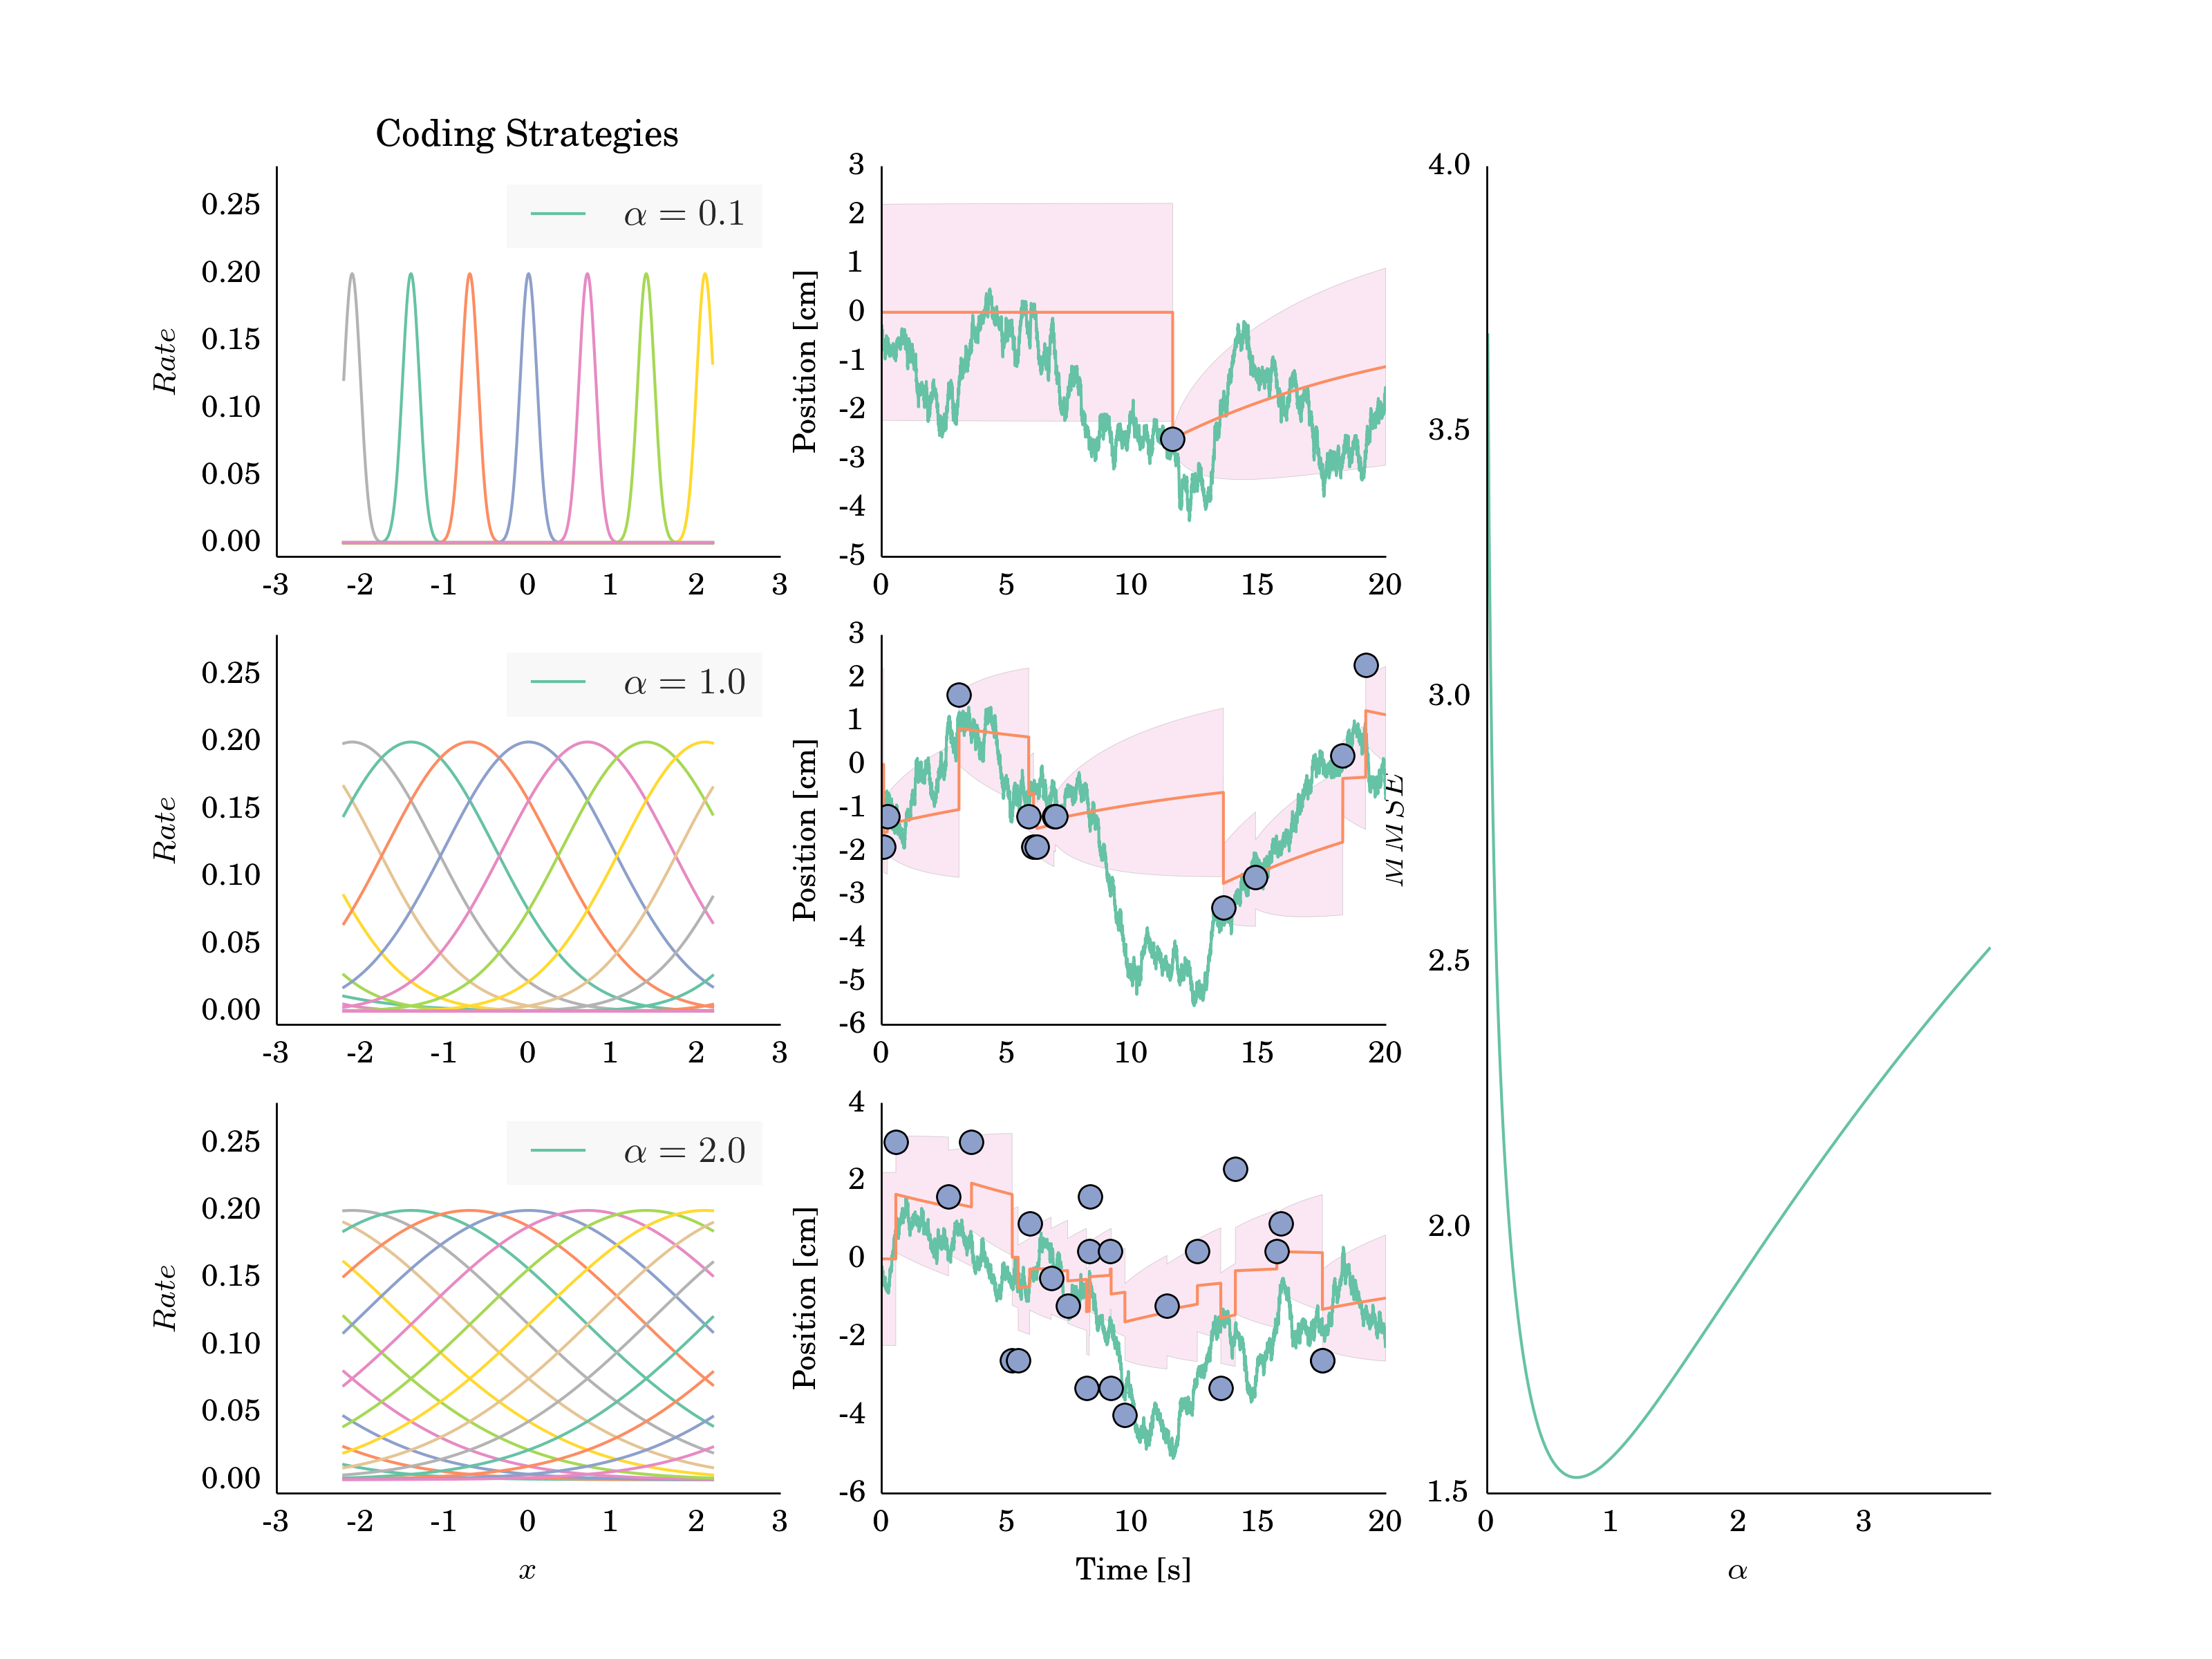
\includegraphics[width=\columnwidth]{figures/figure_5_1.png}
\caption{Optimal coding for filtering Problems: The leftmost column shows the tuning curves of the neurons in the population. Meanwhile, the middle column
shows the general setup of the filtering scheme for each population for the same stochastic process. Note the different situations for narrow and broad tuning curves.
The rightmost plot shows the MMSE as a function of the tuning width $\alpha$.}
\end{figure}

\subsection{Optimal Codes for Control}

In \fref{chap:control} I have introduced the formalism of stochastic optimal control and shown how to extend it to deal with point process observations. In the same way
as one can define an optimal encoder for a filtering problem, one can define an optimal encoder for a control problem. Given a control problem with a cost function given
by
\[
C(\boldsymbol{N}_{[0,T]},U_{[0,T]}) =\boldsymbol{E}\left[ \int_0^T c(X(t),U(\boldsymbol{N}_{[0,t]})) dt\middle| \boldsymbol{N}\right],
\]
we can like above define the optimal encoder to be the one with parameter $\varphi^*$ given by
\[
\varphi^* = \argmin_\varphi C(\boldsymbol{N}_{[0,T]},U_{[0,T]};\varphi).
\]
These can lead to different results than the filtering framework as has been shown in \cite{Susemihl2014}.

\section{Filtering Linear Stochastic Processes through dense Gauss-Poisson Spike Trains}

Let us then consider a linear stochastic process of the type
\[
dX(t) = AX(t) + H^{1/2} dW(t).
\]
Though this may seem as a somewhat restrictive choice, note that a number of processes can be cast into this format. The simple OU process, which I considered in
\fref{chap:mss} is one example, but generalisations to higher dimensions are relatively simple and include, for example, the stochastic damped oscillator. Taking
the matrices
\[
A= \left(\begin{array}{cc} 0 & 1\\ -\omega^2&-\gamma\end{array}\right), \textrm{ and }H= \left(\begin{array}{cc} 0 & 0\\ 0& \eta \end{array}\right),
\]
will lead to a stochastic process with a periodic component. In \fref{fig:stoch_example} a few examples of linear stochastic systems are shown, with a couple of 
samples of each per plot. Note that, although the focus here is on stationary stochastic processes, for which the distribution converges in the limit of long times,
this is by no means a necessity for the analysis at hand. Even for non-stationary processes such as the Wiener process,\marginnote{The Wiener process $W(t)$ has
a covariance that increases linearly with time.} the posterior density can be stationary, allowing us to evaluate the equilibrium MMSE.\par

\begin{figure}
\label{fig:filtering_expl}
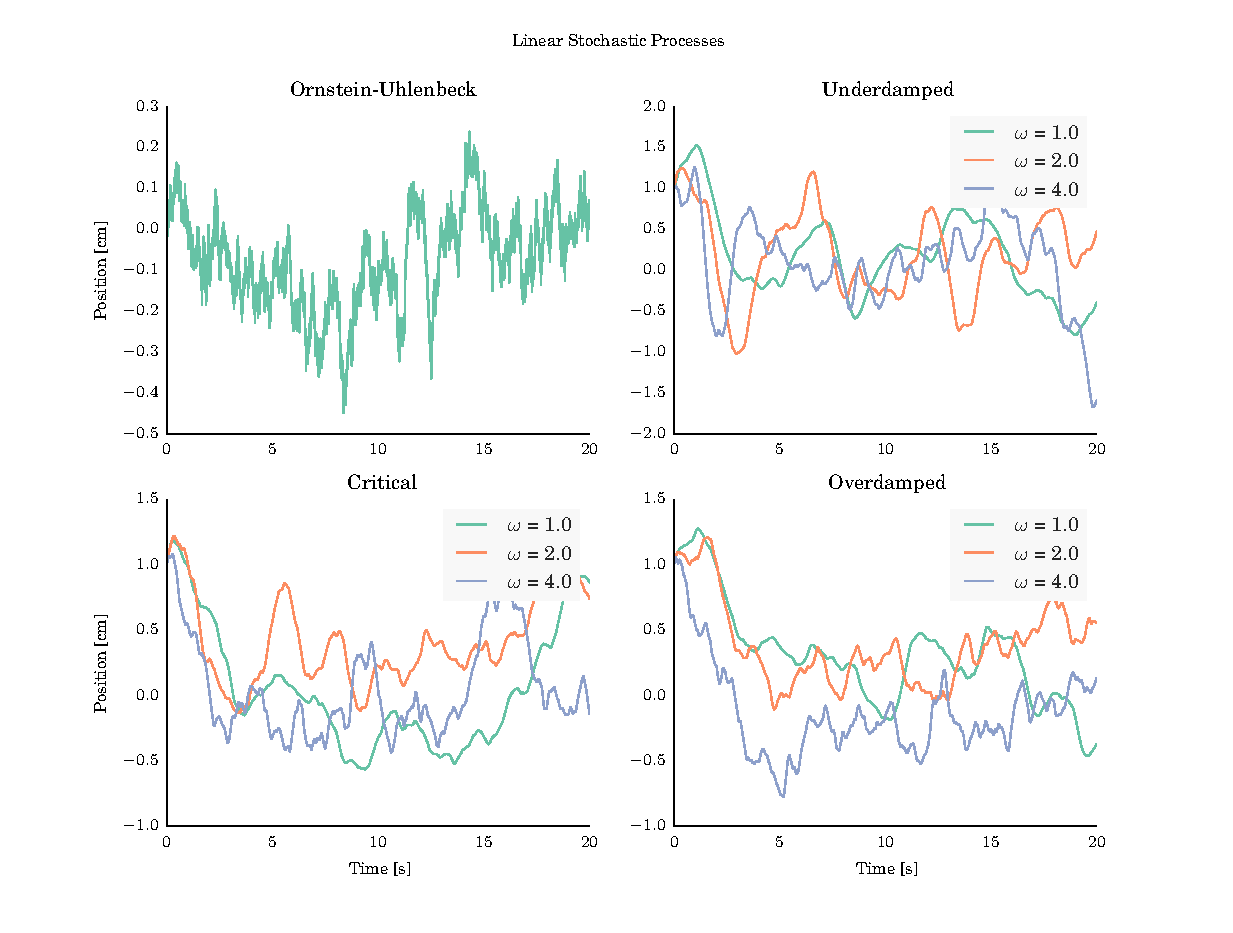
\includegraphics[width=\columnwidth]{figures/figure_5_2.eps}
\caption{Linear stochastic processes: From the top left, we have the one-dimensional Ornstein-Uhlenbeck process, an underdamped stochastic oscillator,
a critically damped stochastic oscillator (bottom left), and an over damped stochastic oscillator.}
\end{figure}


The MMSE $\epsilon(t)$ can then be obtained from the formalism derived in \fref{chap:mse}. Throughout this section I will refer to both the numerical solution of the
evolution equations for $\epsilon(t)$ as well as the mean-field approximation to it. Let me start with the simplest stochastic process, the Ornstein-Uhlenbeck process
given by
\[
dX(t) = -\gamma X(t) dt + \sigma^{1/2} dW(t),
\]
where the evolution of the MMSE is given by
\[
\frac{d\epsilon(t)}{dt} = -2\gamma \epsilon(t) + \sigma -\hat{\lambda} \boldsymbol{E}\left[\frac{s^2}{\alpha^2+s}\right].
\]
We can now consider the temporal evolution of the MMSE, as it has been shown in \fref{fig:matern_coding} for a Matern process. 
We will focus on the equilibrium value of the MMSE, that is, we will focus on the long-term performance of the encoder in the filtering problem, rather than focusing
on the transient, short-time behaviour. Below in \fref{fig:encoder_OU} we can see the equilibrium MMSE of a dense Gauss-Poisson population of neurons encoding
an OU process. The dependence on both the maximal firing rate $\phi$ and the tuning width $\alpha$ is shown.

\begin{figure}
\label{fig:mmse_ou}
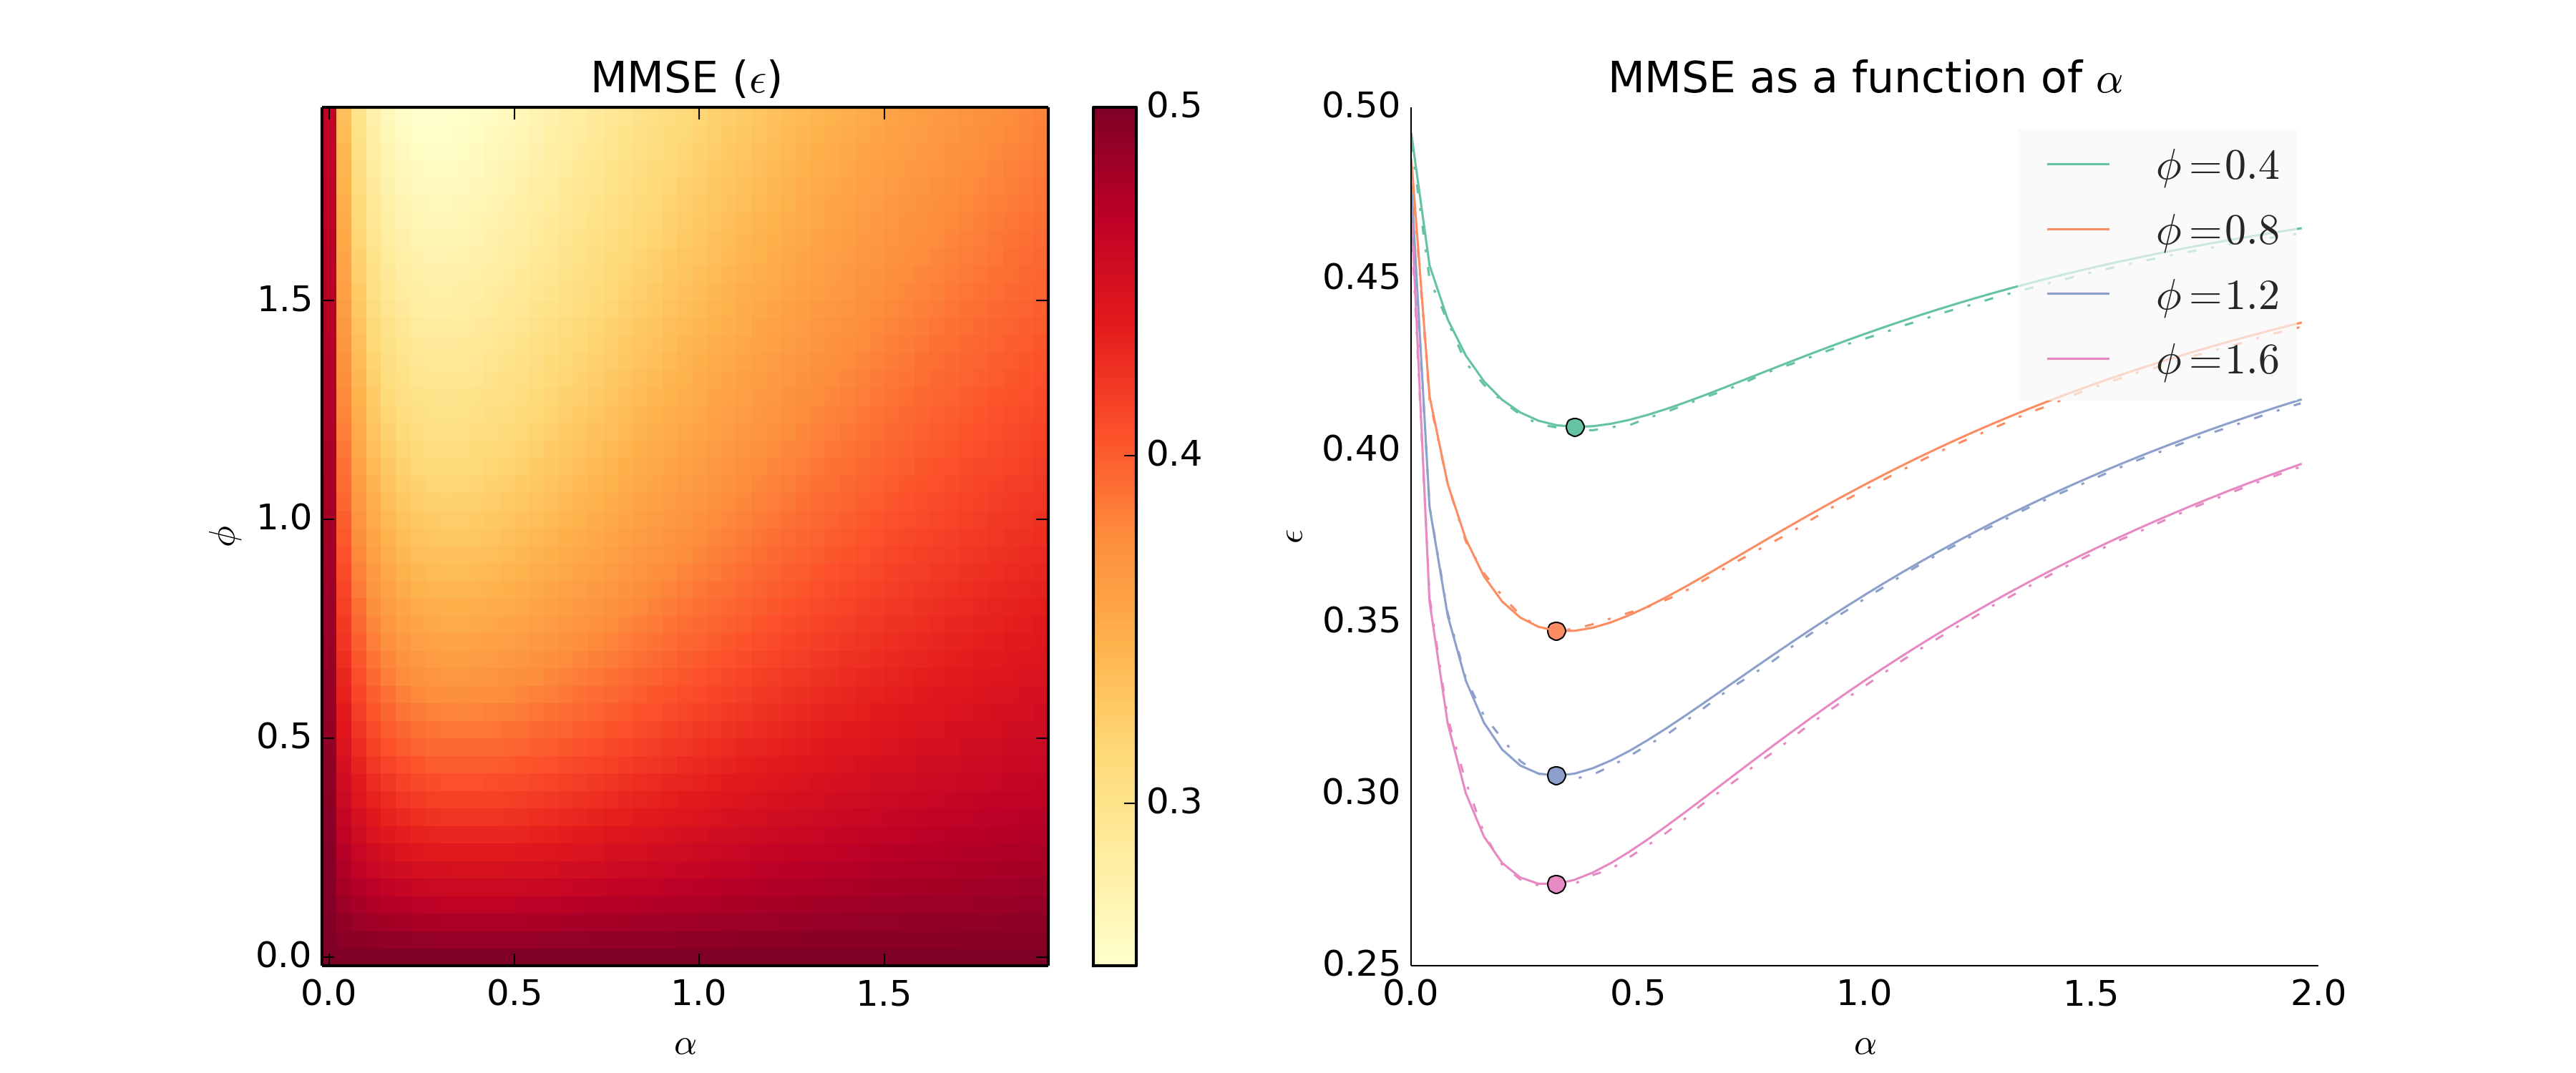
\includegraphics[width=\columnwidth]{figures/figure_5_3.png}
\caption{Comparing Encoders for Filtering: The left hand panel shows a heat map of the MMSE as a function of the maximal firing rate $\phi$ and the tuning
width $\alpha$. There is a trade-off between the number of spikes and the precision of the spikes, manifesting itself in a finite tuning width that minimises the
the MMSE. For any $\alpha$ increasing the firing rate $\phi$ simply decreases the MMSE. The right panel shows the dependence in $\alpha$ for a few values
of $\phi$.}
\end{figure}

More interestingly, we can now ask ourselves how the optimal encoder depends on any of the parameters of the problem. Let us say the parameter $\gamma$
which defines the time-scale of correlations in the OU process.\footnote{Remember that the prior kernel of the OU process is given by $k(s,t) = \frac{\eta^2}{2\gamma} \exp(-\frac{|s-t|}{2\gamma}$.} In \fref{fig:ecological_OU} I have plotted the optimal encoding width $\alpha^*$ as a function of $\gamma$, $\sigma$ and
$\phi$. Though the results are not entirely unexpected, it is interesting to be able to provide an accurate account of the ecological dependence of the optimal 
encoder. Shorter time-scales (larger values of $\gamma$) require a higher frequency of spikes, as the information conveyed by those spikes becomes irrelevant
more quickly. Thus, holding the maximal firing rate $\phi$ fixed, the way to increase the frequency of spikes is to have broader tuning functions. So, as $\gamma$
increases, so does $\alpha^*$.

\begin{figure}
\label{fig:mmse_ou}
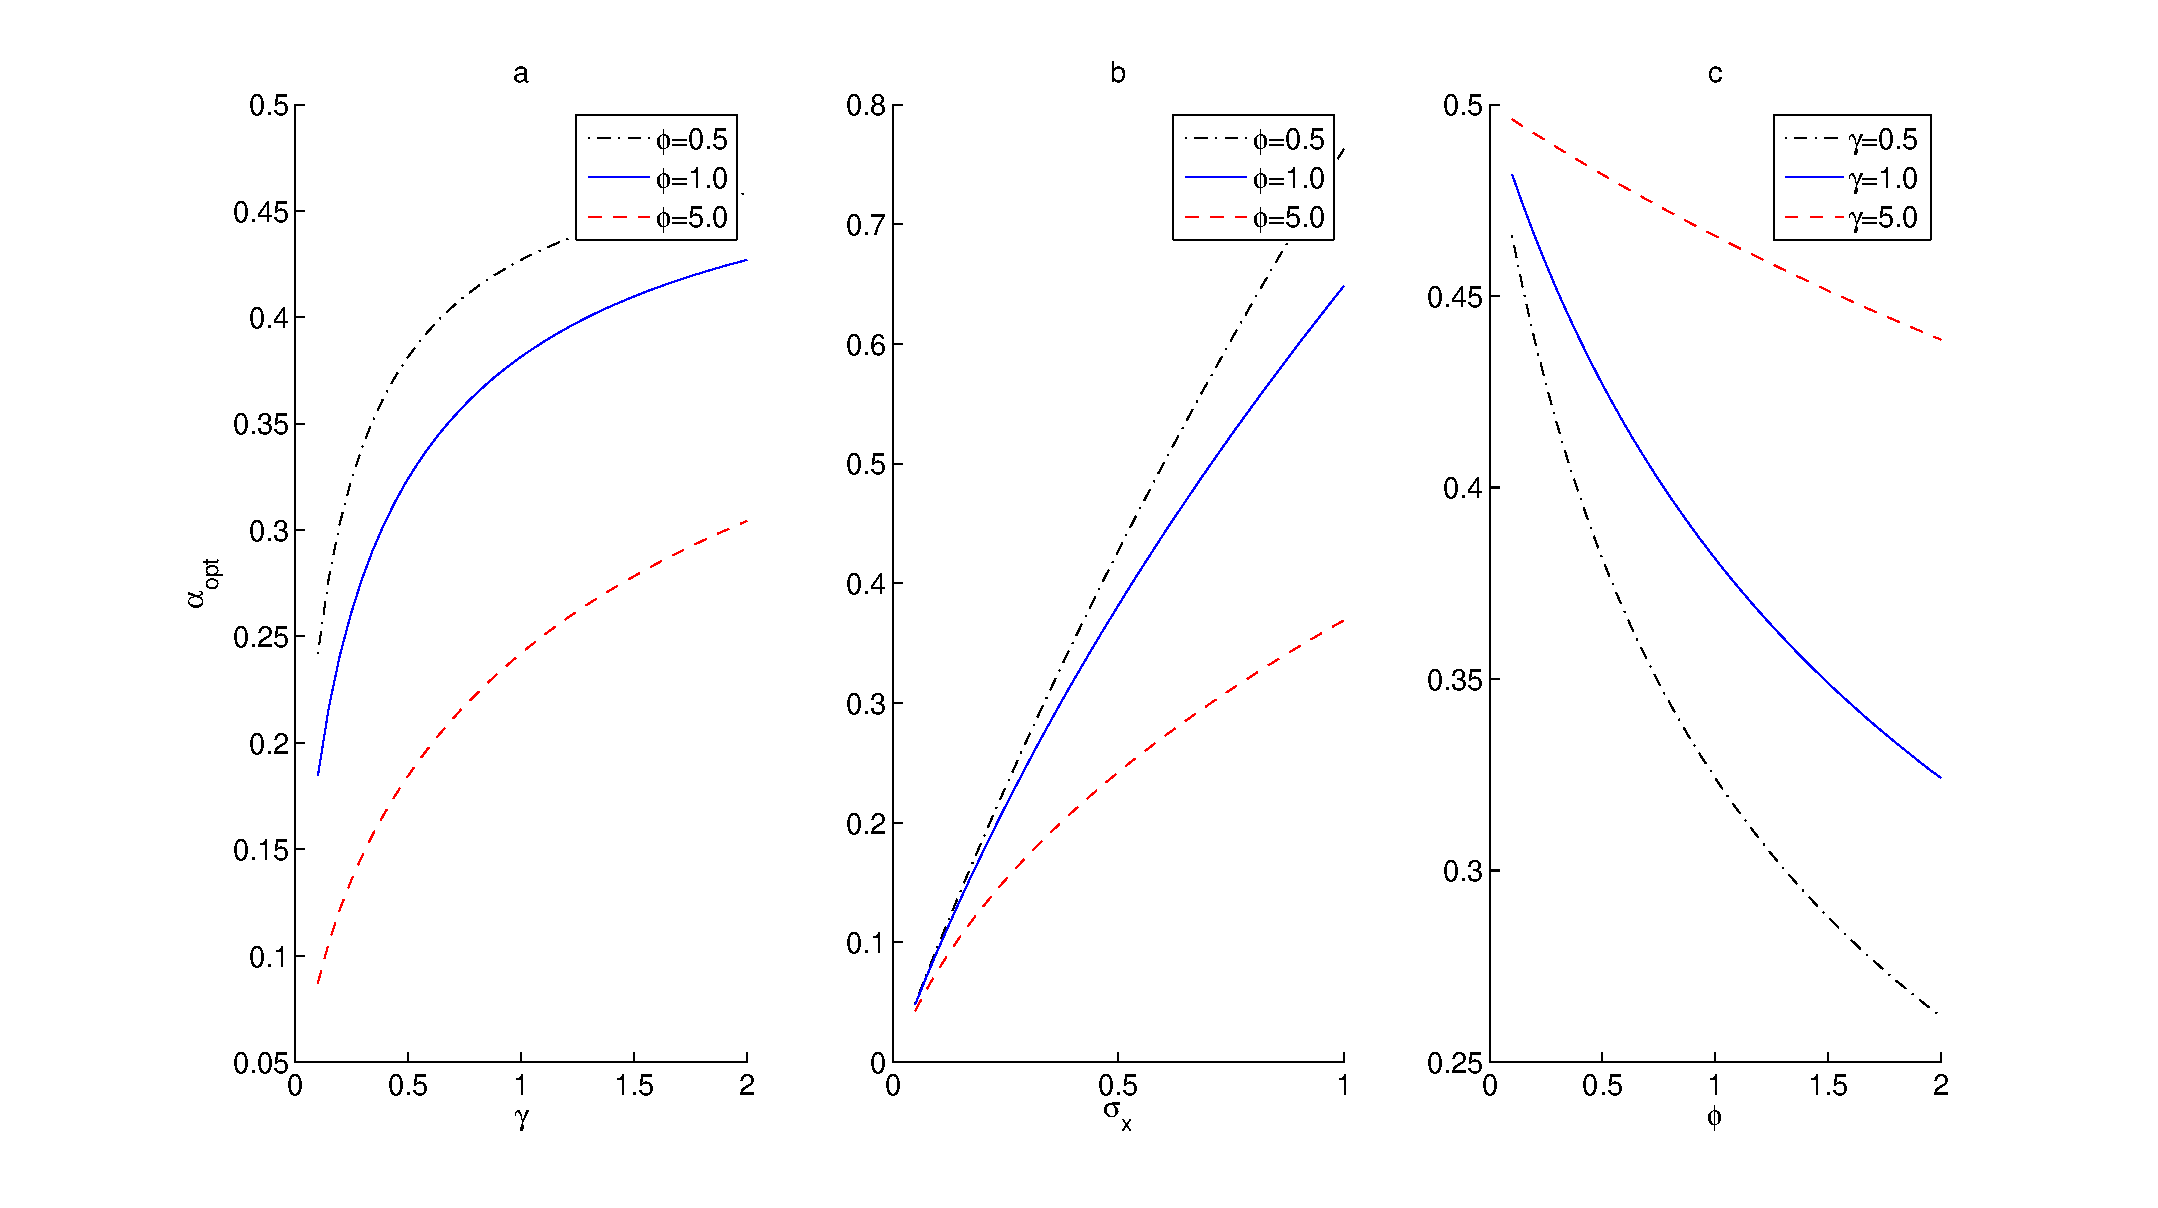
\includegraphics[width=\columnwidth]{figures/figure_5_4.eps}
\caption{Ecological Dependence of the Optimal Encoder:}
\end{figure}

\section{Mean-Field Approach}

\section{Analytic Approaches}

\section{Performance Measures}


\chapter{Discussion}

\section{References}
\bibliography{library}{}
\bibliographystyle{apalike}

\begin{appendices}

\chapter{Proofs}
\section{Maximum Entropy Distributions}
\label{app:entropy}
Let us assume we have a a finite set of outcomes $\mathcal{A}_x = \{x_i\}$, and we wish to find the distribution over $A$ which maximizes the entropy 
\[
H[P_X] = \sum_{x_i} P_X(x_i) \log \left(\frac{1}{P_X(x_i)}\right).
\]
We can use a Lagrange multiplier to enforce the normalization of $P_X(x)$ and then take a derivative with respect to $P_X$. We will have
\[
\mathcal{L}[P_X,\beta] = H[P_X] - \beta \left(\sum_{x_i} P_X(x_i) -1\right).
\]
The derivative of $\mathcal{L}$ with respect to $P_X$ will then give
\[
\frac{\delta \mathcal{L}}{\delta P_X(x_i)} = -\log(P_X(x_i)) + 1 - \beta.
\]
Setting that to zero we will obtain
\[
P_X(x_i) = \exp\left(-1+\beta \right).
\]
This is a uniform distribution, as $\beta$ is a normalization constant and does not depend on $x$. Likewise, if we have any other information about the distribution, such as the expected value of some function of $X$, we can include this as a Lagrange multiplier as well. Generally, if we have a number of functions $f_j(x)$ whose expected value is known to be $e_j$, we can obtain a maximum entropy distribution similarly by writing
\[
\mathcal{L}[P_X,\boldsymbol{\beta}] = H[P_X] - \beta_0 \left(\sum_{x_i} P_X(x_i) -1\right) +  \sum_j \beta_j \left(\sum_{x_i} f_j(x_i) P_X(x_i) -e_j\right).
\]
The derivative will then be given by
\[
\frac{\delta \mathcal{L}}{\delta P_X(x_i)} = -\log(P_X(x_i)) + 1 - \beta_0 - \sum_j \beta_j f_j(x_i).
\]
Which will lead to
\[
P_X(x_i) = \exp\left(-1+\beta_0+\sum_j \beta_j f_j(x_i)\right).
\]
Note that the values of every constant $\beta_j$ has to be determined so that the expected values of $f_j(x)$ match the known values. The Boltzmann distribution is given by this derivation if we require the expected value of the energy of the system to be equal to some expected value, and its associated multiplier will be the inverse temperature $\beta = 1/k_B T$.
\section{LQG Control: The Multidimensional Case}
\label{app:lqg}
If we extend the LQG problem to the multidimensional case we will have the system dynamics
$$
dX_t = (A X_t + B u_t) dt + H dW_t,
$$
where $X_t \in \mathcal{R}^n$, $u_t \in \mathcal{R}^m$, $dW_t \in \mathcal{R}^n$, $A \in \mathcal{R}^{n^2}$, $B \in \mathcal{R}^{nm}$ and $H\in \mathcal{R}^{n^2}$ and positive-definite. We can then write the path cost function as
$$
c(X,u,t) = \frac{1}{2} u^\top R(t) u + \frac{1}{2} X^\top Q(t) X,
$$
and final cost
$$
h(X) = \frac{1}{2} X^\top Q_T X,
$$
where $R: \mathcal{R} \to \mathcal{R}^{m^2}$ and $Q : \mathcal{R}\to \mathcal{R}^{n^2}$ are positive-definite for all $t$.
The HJB equation then becomes
$$
-\frac{\partial V}{\partial t} = \min_{u_t} \left[\frac{1}{2} u_t^\top R(t) u_t + \frac{1}{2} X^\top Q(t) X_t + \frac{\partial V}{\partial X}^\top \left(AX_t  + Bu_t\right) + tr\left(\frac{\partial^2 V}{\partial X^2} H H^\top\right)\right].
$$
Minimization then yields
$$
u^*_t = - R^{-1} B^\top \frac{\partial V}{\partial X}.
$$
Inserting it back we obtain
$$
-\frac{\partial V}{\partial t} =-\frac{1}{2} \frac{\partial V}{\partial X}^\top B R^{-1} B^\top \frac{\partial V}{\partial X}+ \frac{1}{2} X^\top Q(t) X_t + \frac{\partial V}{\partial X}^\top AX_t +  tr\left(\frac{\partial^2 V}{\partial X^2} H H^\top\right).
$$
Then, again assuming that $V(X,t) = X^\top S(t) X + \alpha(t)^\top X + \beta(t)$, we obtain
$$
-\dot{S} = \frac{1}{2} Q(t) - S(t) B R(t)^{-1} B^\top S(t) + S(t) A + A^\top S(t),
$$
$$
-\dot{\alpha} = A^\top \alpha(t) - S(t) BR(t)^{-1} B^\top \alpha(t)
$$
$$
-\dot{\beta} =  tr\left(S H^\top H\right),
$$
where the equation for $S(t)$ is the differential matrix Riccati equation. These must be solved backwards under the boundary conditions $S(T) = Q_T$, $\alpha(T)=0$, $\beta(t) = 0$.
\end{appendices}
\end{document}  
